%-----------------------------------------------------------------------------
\documentclass[12pt,a4paper]{report}
%---------------------------------------------------------------------------
\usepackage{amsmath}
\usepackage{amssymb}
\usepackage{amsthm}
\usepackage{amsfonts}
\usepackage{array}
\usepackage{longtable}
\usepackage{appendix}
\usepackage{blkarray}
\usepackage{bibentry}
\usepackage[none]{hyphenat}
\usepackage[noadjust]{cite}
\usepackage{filecontents}
\usepackage[all,knot,arc,poly]{xy}
\usepackage[pdftex]{graphicx}
\graphicspath{{images/}{../images/}}
\DeclareGraphicsExtensions{.pdf,.jpeg,.png, .jpg}
\usepackage{lscape}
\usepackage{epsfig}
\usepackage{mathrsfs}
\usepackage[left=40mm,right=25mm,top=25mm,bottom=25mm]{geometry}
\usepackage{url}
\usepackage{multicol}
\usepackage{multirow}
\usepackage{color}
\usepackage[table]{xcolor}
\definecolor{pink}{rgb}{1,0.5,0.5}
\usepackage{graphicx}
\graphicspath{ {images/} }
\usepackage{float}
\floatstyle{boxed} 
\restylefloat{figure}

\usepackage{tikz}
\usetikzlibrary{patterns,graphs,arrows.meta,shapes,trees,bending,fadings,quotes,angles}
\usepackage{forest}

% ---------------------------------------------------------------------------
% House diagram style.
%
% The diagrams were drawn over several years and drifted apart: five different
% blues, arrow tips from two different libraries, label sizes ranging from
% \tiny to \large, and line weights from "thin" to "ultra thick". Individually
% each is fine; read one after another they look like they came from different
% books.
%
% Rather than edit 41 pictures by hand, this block redefines the few names they
% already share. Every diagram keeps its own structure and picks up one
% consistent look:
%   * the named colours are repointed at a single palette, so every "blue"
%     curve in the notes is the same blue (and matches the theorem boxes in
%     the stylesheet);
%   * the built-in weight keywords are flattened to a narrow range, so no
%     diagram shouts next to its neighbour;
%   * arrow tips, joins and label size are set once for all pictures.
% ---------------------------------------------------------------------------

% Palette. These match the accent colours used by the web stylesheet.
\definecolor{blue}{HTML}{1D4ED8}    % primary: curves, bars, the main object
\definecolor{red}{HTML}{B91C1C}     % contrast: the second object, highlights
\definecolor{green}{HTML}{12603F}   % agreement / accepted region
\definecolor{orange}{HTML}{A16207}  % annotation, worked-example emphasis
\definecolor{gray}{HTML}{6B7280}    % axes, grids, everything structural
\definecolor{cyan}{HTML}{0E7490}
\definecolor{purple}{HTML}{6D28D9}
\definecolor{pink}{HTML}{DB2777}    % (was rgb 1,0.5,0.5 - too pale to print)

\tikzset{
  every picture/.style={
    font=\small,
    line join=round,
    line cap=round,
    >=Stealth,                      % one arrow tip everywhere
  },
  % Flatten the weight range. The keywords stay valid so no picture needs
  % editing; they just no longer differ by a factor of five.
  thin/.style={line width=0.5pt},
  thick/.style={line width=0.9pt},
  very thick/.style={line width=1.1pt},
  ultra thick/.style={line width=1.3pt},
}


% Required for combinations calculation in pgfplots
\pgfmathdeclarefunction{binom}{2}{%
   \pgfmathparse{factorial(#1)/(factorial(#2)*factorial(#1-#2))}%
}


% Function for Hypergeometric PMF
% parameters: x, N, n, k
\pgfmathdeclarefunction{hypergeom}{4}{%
   \pgfmathparse{binom(#3,#1)*binom(#2-#3,#4-#1)/binom(#2,#4)}%
}


\pgfmathdeclarefunction{nbinom}{3}{%
  \pgfmathparse{factorial(#1-1)/(factorial(#2-1)*factorial(#1-#2)) * (#3^#2) * ((1-#3)^(#1-#2))}%
}

\usepackage{pgfplots}
\pgfplotsset{compat=1.18}

% Second half of the house diagram style (see the block above). It has to sit
% after \usepackage{pgfplots}, which defines \pgfplotsset.
\pgfplotsset{
  every axis/.append style={
    axis lines=left,
    axis line style={gray, line width=0.6pt},
    tick style={gray},
    grid style={dashed, gray!30, line width=0.4pt},
    label style={font=\small},
    tick label style={font=\footnotesize},
    title style={font=\small\bfseries, yshift=2pt},
    legend style={font=\footnotesize, draw=gray!40, fill=white},
    every axis plot/.append style={line width=1pt},
  },
}




\usepackage{rotating}
%-----------------------------------------------------------------------------
\usepackage{setspace}
\usepackage{titletoc}
\titlecontents{chapter}
[0pt]
{\bfseries}
{\MakeUppercase\chaptername\ \thecontentslabel:\quad}
{\MakeUppercase}
{\hfill\contentspage}[]
%-----------------------------------------------------------------------------
\usepackage{float}
\textwidth 6.5in \textheight 9.175in\topmargin 0in \headheight 0in
\oddsidemargin 0in \evensidemargin 0in
\parskip 0.5\baselineskip
\parindent 0pt
\renewcommand{\baselinestretch}{1.25}
%-----------------------------------------------------------------------------
\theoremstyle{definition}
\newtheorem{thm}{Theorem}[section]
\newtheorem{definition}[thm]{Definition}
\newtheorem{example}[thm]{Example}
\newtheorem{exe}[thm]{Exercise}
\newtheorem{note}[thm]{Note}
\newtheorem{remark}[thm]{Remark}
\theoremstyle{plain}
\newtheorem{prop}[thm]{Proposition}
\newtheorem{conj}[thm]{Conjecture}
\newtheorem{coro}[thm]{Corollary}
\newtheorem{lem}[thm]{Lemma}
\newtheorem{tech}{Technique}[section]
\newtheorem{fact}[thm]{Fact}

% ---------------------------------------------------------------------------
% Practice problems taken from past papers.
%
% Each problem records where it came from. That provenance is the point: a
% learner revising from a past paper can see which topic each question belongs
% to, which is the thing they most often cannot work out for themselves.
%
%   \begin{problem}{2019 Exam, Q2}  ... \end{problem}
%   \begin{solution} ... \end{solution}
%
% build.py turns each solution into a collapsed <details> block on the web, so
% the problem can be attempted before the answer is visible.
% ---------------------------------------------------------------------------
% `definition` style, not `plain`: a problem statement is upright text, not an
% italicised assertion. (\theoremstyle is stateful - the block above leaves it
% set to `plain`.)
\theoremstyle{definition}
\newtheorem{problemx}{Problem}[section]
\newenvironment{problem}[1]
  {\begin{problemx}\textup{\small[#1]}\hspace{0.4em}\ignorespaces}
  {\end{problemx}}
% Built on `proof` so it inherits the same quiet styling, but a solution is not
% a proof - it ends with an answer, not a QED square.
\newenvironment{solution}
  {\renewcommand{\qedsymbol}{}\begin{proof}[\textit{Solution}.]}
  {\end{proof}}

\renewcommand{\contentsname}{Contents}
\renewcommand\bibname{REFERENCES}
%\renewcommand{\qedsymbol}{$\blacksquare$}

\parindent 0ex

%-----------------------------------------------------------------------------
\usepackage{titlesec}
\titleformat{\chapter}[hang]
          {\normalfont\filright\ttfamily\scshape\sffamily\bfseries
          	\centering\large}
          {\MakeUppercase{\chaptertitlename}\ \thechapter}{10pt\ :}{\large\MakeUppercase}        
          \titlespacing*{\chapter}{0pt}{-90pt}{16pt}
                       
\titleformat{\section}[hang]
           {\normalfont\sffamily\bfseries%
            \large}
            {\thesection.}{1ex}{}%[\titlerule]
%-----------------------------------------------------------------------------


%-----------------------------------------------------------------------------
%-----------------------------------------------------------------------------
\usepackage{fancyhdr}
\fancyhead{}

\pagestyle{fancy}

\fancyhf{}
%\fancyfoot[C]{\small Prepared by N.~Jeshurun \quad \thepage}

\fancyfoot[R]{\scriptsize Prepared by N.~Jeshurun Mwanza}
\fancyfoot[C]{\thepage}


%\fancyfoot[C]{\small Prepared by N.~Jeshurun}
\renewcommand{\headrulewidth}{0pt}
\renewcommand{\footrulewidth}{0pt}
%-----------------------------------------------------------------------------




%-----------------------------------------------------------------------------

\renewcommand{\sectionmark}[1]{\markright{}} %\thesection\ #1 (this one should be in th brackets, ayoub)
%-----------------------------------------------------------------------------

%-----------------------------------------------------------------------------


\newcommand{\bpf}{\noindent {\ttfamily  PROOF}. $\mbox{}$}
\newcommand{\epf}{\hfill \hbox{\raisebox{.5ex}{$\blacksquare$}$\phantom{.}$}}
%-----------------------------------------------------------------------------
\begin{document}
\pagenumbering{roman}
\begin{titlepage}
%titlepage
\thispagestyle{empty}
\begin{center}

    \centering
%University logo
    %\includegraphics[width=0.3\linewidth]{logo.pdf}

\vspace{4cm}
{\Huge\bfseries Introduction to Probability}

\vspace{0.6cm}
{\Large\itshape Course Notes}

\vfill
{\large Foundations, random variables, and distributions}

\vfill
\textbf{\large 2026}
\end{center}
\clearpage

\pagenumbering{roman} 
\end{titlepage}
%\maketitle












%----------------------------------------------------------------------------------------------------------------------------------------------------

\newpage
%\phantom{.}
%\vspace{20mm}
%\noindent
%Table of contents
\begin{spacing}{1.7}
\tableofcontents
\end{spacing}

\newpage
%\noindent
%\begin{center}
%{\Large\bf Index of Notation} 
%\end{center}

















\newpage
\pagenumbering{arabic}


%--------------------------------------------------------------------------------------------------------------------------------





     
%-------------------------------------------------------------------------------------------------------------------------------------------------------


\chapter{Introduction To Probability}

\section{Introduction}
\vspace{-15pt}
In the scientific investigation of physical phenomena, it is essential to develop mathematical models that facilitate the prediction of observed characteristics. Broadly, these models are categorized into two distinct types: \textit{deterministic} and \textit{non-deterministic (stochastic)}.


\begin{example} \textbf{Deterministic Models} 
A deterministic model is one in which the output is uniquely determined by the initial conditions and parameter values, without any element of randomness.
\begin{enumerate}
\item[(i)] \textbf{Classical Mechanics:} The displacement $s$ of an object under constant acceleration $a$ after time $t$ is given by $s = ut + \frac{1}{2}at^2$.
\item[(ii)] \textbf{Geometry:} The volume $V$ of a sphere is a direct function of its radius $r$, defined by $V = \frac{4}{3}\pi r^3$.
\item[(iii)] \textbf{Ohm’s Law:} The voltage $V$ across a conductor is the product of the current $I$ and the resistance $R$, such that $V = IR$.
\end{enumerate}
\end{example}


\begin{example}[\textbf{Non-deterministic (Stochastic) Models}]  These models account for inherent randomness or uncertainty; even with identical initial conditions, the observed outcomes may vary. 
\begin{enumerate} 
\item[(i)] \textbf{Telecommunications:} The number of data packets arriving at a network server during a peak hour. 
\item[(ii)] \textbf{Reliability Engineering:} The operating lifespan of a semiconductor before failure under standard thermal conditions. 
\item[(iii)] \textbf{Finance and Insurance:} The daily fluctuations of a stock market index or the number of claims filed with an insurer in a fiscal quarter. 
\item[(iv)] \textbf{Public Health:} The transmission rate and number of new infections of a pathogen within a specific population over a six-month period. 
\end{enumerate} 
\end{example}



\begin{note}
The primary objective of probability  is to provide a rigorous mathematical framework for analyzing and modeling these non-deterministic situations
\end{note}



\section{Notation and Terminology}
\begin{definition}
The following are probability terms used:
\begin{enumerate}
\item Random experiment: (also called act, trial, operation, or process) is an activity that leads to the occurrence of one and only one of several possible outcomes which is not likely to be known until its completion.
\item Experiment: Refers to the process of obtaining an observed result of some phenomenon, tossing a coin.
\item Outcome: A possible result of an experiment (e.g., getting a 4 on a die roll).

Only one of the possible outcomes will occur at any given trial of the experiment.

\item Sample Space $S$: Refers to a set of all possible outcomes of an experiment and  denoted by $S$. (e.g., for a die, $S = \{1, 2, 3, 4, 5, 6\})$.

\item Event $E$: A subset of a sample space is called and event. (e.g., rolling an even number, $E=\{2,4,6\})$.
\begin{enumerate}
     \item Events $A_1, A_2, A_3,\cdots, A_n$ are said to be \textit{mutually exclusive}, if $A_j\cap A_i=\emptyset$ then $i\neq j$.
     \item Two or more events are said to be \textit{equally likely} if each has an equal chance to occur.
     \item Two events are said to be \textit{independent} if the occurrence of one does not affect the other.\\
\end{enumerate}
\end{enumerate}
\end{definition}






\begin{example}
\textbf{ }
\begin{enumerate}
\item Tossing of two coins and observe the side which is facing up. What is the sample space?  $${S}=\{HH, HT, TH, TT\}$$ $H=$ head up and $T=$ Tail up.
\item Tossing two coins and observe the number of heads. What is the sample space? $${S}=\{0,1,2\}$$
\item A lot of $N$ items where there are $D$ defectives $(D\leq N)$. The items are selected one by one (without replacement) until the last defective is selected (found) and observe the number of selected items. What is the sample space?$$S=\{D, D+1, D+2,\cdots, N\}$$
\item Light bulb is put on life test and aged to failure (Observe the time it takes fail)$$S=\{t:t\geq 0\},\quad t= \text{time}$$
\end{enumerate}
\end{example}







\section{Definitions and Axioms of Probability}
\begin{definition}
If an experiment gives rise to a sample space $S$ which has finite number of elements $(N)$ of equally likely outcomes, then the probability of an event $E$ denoted by $P(E)$ and is given by $$P(E)=\frac{n(E)}{N},$$ while $n(E)$ is the number of elements in the set $E$.  $P(E)$ is the ratio of number of elements in the set $E$ with the number of elements in $S$.
\end{definition}




\begin{example}
In an experiment of tossing two coins and observing the face up
\begin{enumerate}
\item[(i).] Let the events $A$ be a head up.
\item[(ii).] Let the events $B$ be exactly one tail.
\end{enumerate}
Find the probabilities of (i) and (ii).
\end{example}
\begin{proof}[\textbf{\textit{Solution}}]
The sample space, \[S=\{HH, HT, TH, TT\},\quad N=4.\]
Event is \[A =\{HH, HT, TH\},\quad n(A)=3\] then \[P(A) =\frac{n(A)}{N} =\frac{3}{4}.\]
And \[B =\{HT,TH\},\quad n(B)=2 \]
hence \[P(B) =\frac{2}{4}=\frac{1}{2}.\]
\end{proof}



Another approach to probability involves the conceptual repetitions of an experiment and counting the number of trials and the number of times the event in question occurs.

\begin{definition}
If an experiment is repeated in times and let $M(E)$ be the number of times events $A$ occurs in $M$ trials $\frac{M(E)}{M}$ relative frequency of event $E$ and $\frac{M(E)}{M}$ tends to stabilize as $M$ becomes very large $$P(E)=\lim_{M\longrightarrow \infty}\frac{M(E)}{M}$$ If an experiment has sample space $S$ and an event $E$ defined on $S$ i.e $E\subset S$ then $P(E)$ is a real number called the probability of event $E$.  $P(\cdot)$ is a function whose domain in $S$ and range is $[0,1]$ $$P:S\longrightarrow [0,1]$$
\end{definition}





\subsection{Axioms of probability}
\begin{enumerate}
\item[(i).] For any event $E$, $0\leq P(E)\leq 1$.
\item[(ii).] $P(S)=1$.
\item[(iii).] For any finite number of mutually exclusives events $E_1, E_2,...,E_k$ then $$P\left(\bigcup^k_{j=1}E_j\right)=\sum_{j=1}^k P(E_j).$$
\end{enumerate}




\begin{note}
\[\bigcup^k_{j=1}E_j  = E_1\cup E_2\cup E_3\cup \cdots \cup E_k\]
\[\sum^k_{j=1}P(E_j)  = P(E_1)+ P(E_2) + \cdots +P(E_k)\]
\end{note}



\begin{thm}
Let $A$ and $B$ be any set events and $S$ be the sample space of an experiment then
\begin{enumerate}
\item[(i).] $P(\emptyset)=0\,$ where $\,\emptyset\,$ is empty set.
\item[(ii).] $P(A')=1-P(A)$
\item[(iii).] $P(A\cup B)=P(A)+P(B)-P(A\cap B)$
\item[(iv).] if $A\subset B$ $\implies$ $P(A)\leq B$
\end{enumerate}
\end{thm}


\begin{proof}
We prove (iii), we express $A\cup B$, $A$ and $B$ as 
\begin{equation}
A\cup B=(A\cap B') \cup (A\cap B) \cup (A'\cap B)
\end{equation}
\begin{equation}
A =(A\cap B) \cup (A\cap B')
\end{equation}
\begin{equation}
B =(A\cap B) \cup (A'\cap B)
\end{equation}
From the three equations we get
\begin{align*}
P(A\cup B) &=P(A\cap B') + P(A\cap B) + P(A'\cap B)\\
P(A) &=P(A\cap B) + P(A\cap B')\\
P(B) &=P(A\cap B) + P(A'\cap B)
\end{align*}
Therefore 
\begin{align*}
P(A\cup B) &=P(A)-P(A\cap B)+P(A\cap B)+P(B)-P(A\cap B)\\
           &=P(A)+P(B)-P(A\cap B).
\end{align*}
\end{proof}




\begin{example}
If event $A$ and $B$ are such that $P(A)=0.3$, $P(B)=0.6$ and $P(A\cup B)=0.8$, evaluate the following
\begin{enumerate}
\item[(i).] $P(A')$
\begin{proof}[\textbf{\textit{Solution}}]
$P(A')=1-P(A)=1-0.3=0.7$
\end{proof}       
       
\item[(ii).] $P(A\cap B)$
\begin{proof}[\textbf{\textit{Solution}}]
$P(A\cap B)  = P(A)+P(B)-P(A\cup B) = 0.3+0.6-0.8 = 0.1$
\end{proof}

\item[(iii).] $P(A'\cup B')$
\begin{proof}[\textbf{\textit{Solution}}]
$P(A'\cup B')  = P\left((A\cap B)\right)'  = 1-P(A\cap B) = 1-0.1 = 0.9$
\end{proof}

\item[(iv).] $P(A'\cap B')$
\begin{proof}[\textbf{\textit{Solution}}]
$P(A'\cap B') = P\left((A\cup B)'\right) = 1-P(A\cup B) = 1-0.8 = 0.2$
\end{proof}
\end{enumerate}
\end{example}



\begin{example}
The Samsung cell phones require replacement of possible defects of the LCD and in the charging system defects. Samsung have being informed that $2\%$ of the phones have defective LCD only and $4\%$ have defective charging system only. If $90\%$ of these phones have neither defective, what percentage of these have both defects?
\end{example}



\begin{proof}[\textbf{\textit{Solution}}]
Let $A$ be the event of a defective LCD and $B$ be the event of a defective charging system. 
We are given:
\begin{itemize}
    \item $P(A \cap B') = 0.02$ (Defective LCD \textit{only})
    \item $P(B \cap A') = 0.04$ (Defective charging \textit{only})
    \item $P((A \cup B)') = 0.90$ (Neither defective)
\end{itemize}

First, find the probability that a phone has at least one defect:
\[ P(A \cup B) = 1 - P((A \cup B)') = 1 - 0.90 = 0.10 \]



We know that $P(A \cup B)$ is the sum of the disjoint regions:
\[ P(A \cup B) = P(A \cap B') + P(B \cap A') + P(A \cap B) \]
\[ 0.10 = 0.02 + 0.04 + P(A \cap B) \]
\[ P(A \cap B) = 0.10 - 0.06 = 0.04 \]

\textbf{Conclusion:} $4\%$ of the phones have both defects.
\end{proof}
















\section{Independent Events, Conditional Probability and Bayes' Theorem}
\subsection{Independent Events}
\begin{definition}
Events $A$ and $B$ are said to be independent if and only if $P(A\cap B)=P(A)P(B)$.
\end{definition}

\begin{lem}
 Two events $A$ and $B$ are independent if and only if $P(A\cap B)=P(A)P(B)$.
\end{lem}


\begin{thm}
If $A$ and $B$ are independent then the following are also independent
\begin{enumerate}
\item[(i).] $A$ and $B'$
\begin{proof}
We know that $P(A\cap B)=P(A)P(B)$, since $A$ and $B$ are independent.
\[A =(A\cap B')\cup (A\cap B)\]
\[P(A) =P(A\cap B')+P(A\cap B)\]
Therefore
\begin{align*}
P(A\cap B') &=P(A)-P(A\cap B)\\
            &=P(A)-P(A)P(B)\\
            &=P(A)(1-P(B))\\
            &=P(A)P(B').
\end{align*}
i.e $P(A\cap B')=P(A)P(B')$ implies $A$ and $B'$ are independent.
\end{proof}


\item[(ii).] $A'$ and $B$
\begin{proof}
Write $B =(A'\cap B)\cup (A\cap B)$, then $P(B) = P(A'\cap B)+P(A\cap B)$
\begin{align*}
P(A'\cap B) &=P(B)-P(A\cap B)\\
            &=P(B)-P(A)P(B)\\
            &=P(B)(1-P(A))\\
            &=P(B)P(A').
\end{align*}
i.e $A'$ and $B$ are independent.
\end{proof}



\item[(iii).] $A'$ and $B'$
\begin{proof}
Write $A'  = (A'\cap B)\cup (A'\cap B')$, then 
\[P(A') =P(A'\cap B)+P(A'\cap B')\]
\begin{align*}
P(A'\cap B') &=P(A')-P(A')P(B)\\
             &=P(A')(1-P(B))\\
             &=P(A')P(B').
\end{align*}
i.e $PA'$ and $B'$ are independent.
\end{proof}
\end{enumerate}
\end{thm}




\subsection{Conditional Probabilities}
The probability properties discussed so far relate to the entire sample space. We have used the symbol $P(A)$ and will continue to do so however we should have been more precise and used $P(A/S)$ to read `` probability of $A$ given the sample space $S$''.

The following definition justifies why $P(A/S)$ is simply $P(A)$ if $S$ is the sample space.




\begin{definition}
Given a sample space $S$, and events $A$ and $B$, then the conditional probability of $A$ given $B$ is denoted by $P(A/B)$ and is given by 
\[P(A/B) =
\begin{cases}
\dfrac{P(A\cap B)}{P(B)} & \text{if}\hspace{0.2cm} P(B)>0\\\\
0 &\text{if}\hspace{0.3cm} P(B)=0\\
\end{cases}\]
\end{definition}


\begin{thm}
If $A$ and  $B$ are independent events, then
\[P(A/B)  =\frac{P(A\cap B)}{P(B)} = \frac{P(A)P(B)}{P(B)} = P(A).\]
\end{thm}



\begin{remark}
We have $P(A\cap B)=P(B)P(A/B)$ this is known as multiplicative rule of probability.
\end{remark}



\begin{definition}
If $B_1, B_2, \cdots, B_k$ are mutually exclusive events of the sample space $S$ and if $$\bigcup\limits^k_{j=1}B_j=S,$$ then $B_1, B_2, \cdots, B_k$ are said to be a partition of the sample space $S$.
\end{definition}




\begin{thm}[\textbf{Total Probability}]
If $B_1, B_2,\cdots B_k$ is a partition of the sample space $S$ and $A$ is an arbitrary event on $S$ then the probability of $A$ is given by 
\begin{align*}
P(A) &=\sum^k_{j=1}P(B_j)P(A/B_j)\\
     &=P(B_1)P(A/B_1) +P(B_2)P(A/B_2)+ \cdots +P(B_k)P(A/B_k).
\end{align*}
\end{thm}


\begin{proof}
Let $S$ be a sample space and $A$ be an event in $S$. Then for a partition  $B_1, B_2, \cdots , B_k$ of $S$. We have
\[A = (A\cap B_1)\cup (A\cap B_2)\cup (A\cap B_3)\cup\cdots \cup (A\cap B_k) =\bigcup^k_{j=1}(A\cap B_j)\]
Therefore
\[P(A) =\sum^k_{j=1}P(A\cap B_j) =\sum^k_{j=1}P(B_j)P(A/B_j).\]
\end{proof}




\subsection{Bayes theorem}
There are many  situations where the ultimate outcome of an experiment depends on what happens in various intermediate stages. This issue is resolved by the Bayes' Theorem.
\begin{definition}[\textbf{Bayes theorem}]
If $B_1, B_2, ...... ,B_k$ is a partition of the sample space $S$ and $A$ is an arbitrary event on $S$, then \[P(B_r/A)=\frac{P(B_r)P(A/B_r)}{\sum\limits_{j=1}^kP(B_j)P(A/B_j)}\, , \quad r = 1, 2, \cdots , k.\]
\end{definition}

\begin{proof}
From the definitions of conditional probability and total probability, we obtain 
\[P(B_r/A) =\frac{P(B_r\cap A)}{P(A)} = \frac{P(B_r)P(A/B_r)}{\sum\limits^k_{j=1}P(B_j)P(A/B_j)}.\]
\end{proof}


\begin{note}
In the Bayes Theorem, the probability $P(B_j)$ is called prior probability. The Probability $P(B_j/A)$ is called posterior probability.
\end{note}




\begin{example}
In a factory for manufacturing of car batteries, machines $A$, $B$ and $C$ manufacture respectively $25\%$, $35\%$ and $40\%$ of the total produce. The Percentage of defective batteries from machine $A$, $B$ and $C$ are 5, 4 and 2 respectively.
\begin{enumerate}
\item[(i).] A car battery is selected at random. What is the probability that it is defective?
\begin{proof}[\textbf{\textit{Solution}}]
Machines are the partitions: $A$, $B$, $C$. Let $D$ represent the battery is defective. Given  \[P(A)=0.25,\quad\quad P(B)=0.35,\quad\quad P(C)=0.40,\] \[P(D/A)=0.05, \quad P(D/B)=0.04, \quad P(D/C)=0.02\] Then 
\begin{align*}
P(D) & = P(A)\,P(D/A)+P(B)\, P(D/B)+P(C)\, P(D/C)\\
     &= 0.25\times 0.05 + 0.35\times 0.04 + 0.40\times 0.02\\
     &=0.0125+0.014+0.008\\
     &=0.0345
\end{align*}
\end{proof}


\item[(ii).] A car battery is selected at random and found to be defective. What is the probability that it was manufactured by machine $B$?
\begin{proof}[\textbf{\textit{Solution}}]
\begin{align*}
P(B/D) &=\frac{P(B)P(D/B)}{P(D)}\\
       &=\frac{(0.35\times 0.04)}{0.0345}\\
       &=\frac{0.0140}{0.0345}\\
       &=\frac{28}{69}
\end{align*}
\end{proof}


\item[(iii).] Battery is selected at random and found to be non-defective. What is the probability that it was manufactured by machine $A$?
\begin{proof}[\textbf{\textit{Solution}}]
You can use the tree diagram to find $P(D')$ 

\begin{figure}[H]
\centering
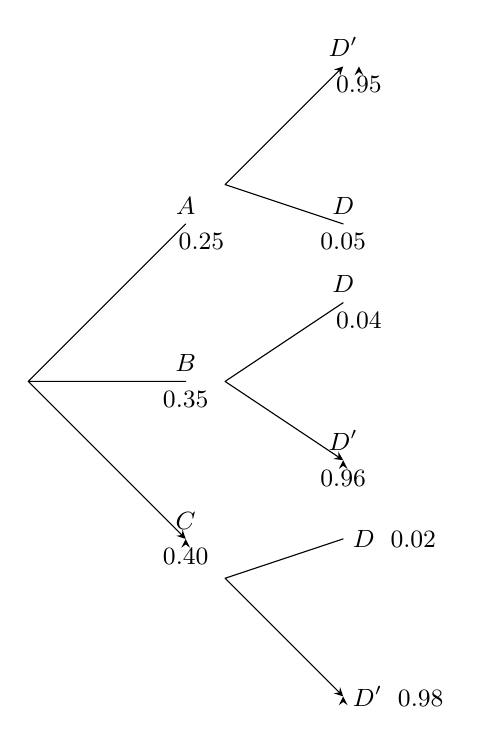
\begin{tikzpicture}[->,>=stealth]
\draw(0,0)--(2,2)
(0,0)--(2,0)
(0,0)--(2,-2);
\draw(2,2)node[above]{$A$}
(2.2,2)node[below]{0.25}
(2,0)node[above]{$B$}
(2,0)node[below]{0.35}
(2,-2)node[above]{$C$}
(2,-2)node[below]{0.40};
\draw(2.5,0)--(4,1)
(2.5,0)--(4,-1);
\draw(4,1)node[above]{$D$}
(4.2,1)node[below]{0.04}
(4,-1)node[above]{$D'$}
(4,-1)node[below]{0.96};
\draw(2.5,2.5)--(4,2)
(2.5,2.5)--(4,4);
\draw(4,2)node[above]{$D$}
(4,2)node[below]{0.05}
(4,4)node[above]{$D'$}
(4.2,4)node[below]{0.95};
\draw(2.5,-2.5)--(4,-2)
(2.5,-2.5)--(4,-4);
\draw(4,-2)node[right]{$D\hspace{0.2cm} 0.02$}
(4,-4)node[right]{$D'\hspace{0.2cm} 0.98$};
\end{tikzpicture}
\end{figure}
Or you can use the fact that $P(D') = 1- P(D)$.
\begin{align*}
P(A/D') & = \frac{P(A)\, P(D'/A)}{P(D')}\\
& = \frac{0.25\times 0.95}{1 - 0.0345}\\
& = \frac{475}{1931}\\
& =0.246
\end{align*}
\end{proof}
\end{enumerate}
\end{example}






\subsection{Contingency Tables}
A Contingency Table is a tabular method used to classify sample observations according to two or more identifiable categories. In the case of two variables, the table rows represent the levels of one variable, and the columns represent the levels of the other. The intersections (cells) represent the joint probability of those specific events occurring simultaneously.

Purpose of Contingency Tables:
\begin{enumerate}
\item To organize complex joint event data into a readable format.
\item The row and column totals (margins) provide the probabilities of a single event occurring, regardless of the other variable.
\item They provide the raw data necessary to determine if two categorical variables are associated.
\end{enumerate}


\begin{example}
To investigate the relationship between smoking and health outcomes, let $A$ be the event that an individual smokes ($A^c$ for non-smokers) and $D$ be the event that an individual develops lung cancer ($D^c$ for no cancer).
If the probability that 
\begin{enumerate}
\item[(i).] an individual smokes and develops lung cancer is 0.15.
\item[(ii).] an individual smoke and doesn't develops lung cancer is 0.25.
\item[(iii).] an individual doesn't smoke and develops lung cancer is 0.10.
\item[(iv).] and individual doesn't smoke and doesn't develop lung cancer is 0.50. 
\end{enumerate}

How can this information be used to examine, the relationship between smoking and lung cancer?
\end{example}

\begin{proof}[\textbf{\textit{Solution}}]
We are given the following joint probabilities: \[P(A \cap D) = 0.15,\quad P(A \cap D^c) = 0.25,\quad P(A^c \cap D) = 0.10,\quad P(A^c \cap D^c) = 0.50\]

\subsubsection{Step 1: Construct the probability table.}
By summing the rows and columns, we obtain the marginal probabilities $P(A)$ and $P(D)$.
\begin{table}[H]
\centering\renewcommand{\arraystretch}{1.5}
\begin{tabular}{|l|c|c|c|}
\hline
\textbf{Smoking Status} & \textbf{Cancer ($D$)} & \textbf{No Cancer ($D^c$)} & \textbf{Marginal Totals}\\ 
\hline
\textbf{Smoker ($A$)} & $0.15$ & $0.25$ & $P(A) = 0.40$\\ 
\hline
\textbf{Non-Smoker ($A^c$)} & $0.10$ & $0.50$ & $P(A^c) = 0.60$\\ 
\hline
\textbf{Marginal Totals} & $P(D) = 0.25$ & $P(D^c) = 0.75$ & $\mathbf{1.00}$\\ 
\hline
\end{tabular}
\caption{Contingency table of Smoking and Lung Cancer probabilities.}
\end{table}


\subsubsection{Step 2: Comparative Analysis (Relative Risk)}
To see how smoking affects cancer risk, we compare the conditional probabilities:

Risk for Smokers $$P(D|A) = \frac{P(A \cap D)}{P(A)} = \frac{0.15}{0.40} = 0.375$$
Risk for Non-Smokers $$P(D|A^c) = \frac{P(A^c \cap D)}{P(A^c)} = \frac{0.10}{0.60} \approx 0.167$$
The Relative Risk (RR):$$ RR = \frac{P(D|A)}{P(D|A^c)} = \frac{0.375}{0.1667} = 2.25 $$
An individual who smokes is 2.25 times more likely to develop lung cancer than a non-smoker.


\subsubsection{Step 3: The Odds Ratio (OR)}
In epidemiology, we often use the Odds Ratio (or Cross-Product Ratio) to estimate the strength of association. For a table with cells $a, b, c, d$:$$ OR = \frac{a \times d}{b \times c} = \frac{0.15 \times 0.50}{0.25 \times 0.10} = \frac{0.075}{0.025} = 3 $$


While the Relative Risk (2.25) tells us how much the probability increases, the Odds Ratio (3.0) provides a different mathematical perspective on the strength of the link. Since $OR \neq 1$, we can conclude that smoking and lung cancer are not independent events.
\end{proof}









\section{Counting Techniques}
In the classical definition of probability, $P(E) = \frac{n(E)}{N}$, we must be able to count the number of outcomes in the event space and the sample space. When the number of outcomes is too large to list manually, we use \textit{counting techniques} or \textit{combinatorial analysis}.


\subsection{Multiplication Principle}
If an operation can be performed in $n_1$ ways, and for each of these a second operation can be performed in $n_2$ ways, then the two operations can be performed together in $n_1 \times n_2$ ways.

If there are $k$ operations, the total number of ways is $n_1\times n_2 \times \cdots \times n_k$.


\begin{example}
Find the number of possible outcomes of the rolling of a die and then a tossing a coin.
\end{example}

\begin{proof}[\textbf{\textit{Solution}}]
Here $n_1= 6$ and $n_2 = 2$. By the multiplication principle, the number of possible outcomes is $6 \times 2 = 12$. 




\begin{figure}[H]
\centering
\begin{forest}
  for tree={
    grow'=east, % Grows from left to right
    parent anchor=east,
    child anchor=west,
    edge={-stealth},
    l sep=2cm, % Length between levels
    s sep=0.1cm, % Spread between branches
    font=\small
  }
  [Start
    [1
      [H, edge label={node[midway,above,font=\tiny]{Toss}} [{1H}, font=\bfseries]]
      [T, edge label={node[midway,below,font=\tiny]{Toss}} [{1T}, font=\bfseries]]
    ]
    [2
      [H [{2H}, font=\bfseries]]
      [T [{2T}, font=\bfseries]]
    ]
    [3
      [H [{3H}, font=\bfseries]]
      [T [{3T}, font=\bfseries]]
    ]
    [4
      [H [{4H}, font=\bfseries]]
      [T [{4T}, font=\bfseries]]
    ]
    [5
      [H [{5H}, font=\bfseries]]
      [T [{5T}, font=\bfseries]]
    ]
    [6
      [H [{6H}, font=\bfseries]]
      [T [{6T}, font=\bfseries]]
    ]
  ]
\end{forest}
\caption{Tree Diagram for Rolling a Die and Tossing a Coin}
\end{figure}
\end{proof}


\begin{example}
How many different license plates are possible if Lusaka uses three letters followed by two digits.
\end{example}
\begin{proof}[\textbf{\textit{Solution}}]
\[(26)^3(10)^2 = 1,757,600\]
\end{proof}





\subsection{Permutations}
A permutation is an arrangement of all or part of  a set of objects in a specific order. The order of selection matters and one permutation differs from another permutation.


\begin{definition}
The number of permutations of $n$ distinct objects taken $k$ at a time is denoted by $_nP_k$ or $P(n,k)$ or $P^n_k$ and is given by:$$ _nP_k = \frac{n!}{(n-k)!} $$where $n!$ (n-factorial) is $n \times (n-1) \times \cdots \times 1$. By definition, $0! = 1$.\end{definition}


\begin{example}
Suppose that there are 4 objects: $p,q,r,s$ $-$ then the possible arrangements of these objects if 3 are taken at a time are:
$n = 4$ and $k = 3$ \[_nP_k = \frac{n!}{(n - k)!}=\frac{4!}{(4-3)!} = \frac{4\times 3\times 2\times 1!}{1!}=24.\]
There are 24 arrangements; permutations of four things taken three at a time.
\begin{table}[H]
\centering
\begin{tabular}{cccc}
$pqr$ & $pqs$ & $prs$ & $qrs$\\
$prq$ & $psq$ & $psr$ & $qsr$\\
$qrp$ & $qsp$ & $rsp$ & $rsq$\\
$qpr$ & $qps$ & $rps$ & $rqs$\\
$rqp$ & $sqp$ & $srp$ & $srq$\\
$rpq$ & $spq$ & $spr$ & $sqr$\\
\end{tabular}
\end{table}
\end{example}





\begin{definition}
Suppose there are $n$ objects, where $k_1$ are of one type, $k_2$ are  of another type, $\cdots$ , $k_m$ are the $m^{\text{th}}$ type, where $k_1+k_2+\cdots +k_m=n$.
 
The number of distinct permutations of $n$ objects is denoted by $\, P^n_{k_1,k_2,\cdots,k_m}\,$ and is given by $$P^n_{k_1,k_2,\cdots,k_m}=\frac{n!}{k_1!k_2!\cdots k_m!}.$$
\end{definition}




\begin{example}
\begin{enumerate}
\item[(a).] How many different ways can 3 red, 4 yellow and 2 blue light bulbs be arranged on a string of tree lights with nine sockets.
\begin{proof}[\textbf{\textit{Solution}}]
We have $\, k_1 = 3, \quad k_2 = 4, \quad k_3  = 2\,$ and $\, n = 3+ 4 + 2$
$$P^n_{k_1,k_2,k_3}=\frac{n!}{k_1!\,k_2!\,k_3!}$$ $$P^9_{3,4,2}=\frac{9!}{3!4!2!}=\frac{9\times 8\times 7\times 6\times 5\times 4!}{3\times 2\times 1\times 2\times 1\times 4!}=1260.$$
\end{proof}

\item[(b).] How many different ways can seven female students on a field trip course be assigned to one triple room and two double rooms at a guest house.
\begin{proof}[\textbf{\textit{Solution}}]
The seven students are being partitioned into three distinct groups: one group of 3 (the triple room) and two groups of 2 (the double rooms).
We have $k_1 = 3, \quad k_2 = 2,\, \quad k_3 = 2$ and $\, n = 7$
\[P^n_{k_1,\,k_2,\, k_3} = \frac{n!}{k_1!\, k_2!\, k_3!}\]
\[P^7_{3,2,2} = \frac{7!}{3!\, 2!\, 2!}=\frac{7\times 6\times 5\times 4\times 3!}{3!\times 2\times 2}=210.\]
\end{proof}
\end{enumerate}
\end{example}




\subsection{Combinations}
\vspace{-15pt}
A combination is a selection of objects where the order does not matter. We are only interested in which objects are chosen, not the sequence in which they are picked.

\begin{definition}
The number of combinations of $n$ distinct objects taken $k$ at a time is denoted by $^nC_k$, $\binom{n}{k}$, or $C(n,k)$ and is given by:$$ \binom{n}{k} = \frac{n!}{k!(n-k)!}.$$
\end{definition}



\begin{remark}
\textbf{  }
\begin{enumerate}
\item Express the permutation as a combination \[P^n_k = k!\, \binom{n}{k}.\]
\item Let $n\in \mathbb{N}$ and $k = 0, 1, 2, \cdots, n$. Then \[\binom{n}{k} = \binom{n}{n-k}.\]
\item For any positive integer $n$ and $k = 1, 2, 3 , \cdots, n$, we have \[\binom{n}{k} = \binom{n - 1}{k} + \binom{n - 1}{k - 1}.\]
\item Let $m$ and $n$ be positive integers. Then % Vandermonde's identity: the sum is C(m+n, k), not C(m+n, n).
\[\sum^k_{r = 0}\binom{m}{r}\binom{n}{k-r} = \binom{m+n}{k}.\]
\end{enumerate}
\end{remark}






\begin{example}
A production lot of size 100 has $5\%$ defective items. A random sample of size 10  is selected (without replacement). Let $A$ be the event that there are exactly 2 defective, $B$ be the event that there are no defectives and $C$ be the event that there are at most 2 defectives. $D$ event that  there is at least 2 defectives. Find the probabilities of $A, B$ and $C, D$.
\end{example}





\begin{proof}[\textbf{\textit{Solution}}]
Let $N = 100$, \, with $D= 5$ defectives and $n-D = 95$ non-defectives. We select $n=10$.

Possible ways of the samples $\binom{100}{10}$.

% diagram 2
\begin{figure}[H]
\centering
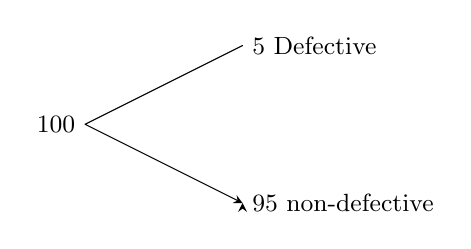
\begin{tikzpicture}[->,>=stealth]
\draw(0,0)--(2,1)
(0,0)--(2,-1);
\draw(0,0)node[left]{100}
(2,1)node[right]{5 Defective}
(2,-1)node[right]{95 non-defective};
\end{tikzpicture}
\end{figure}


\subsubsection{$A$: Exactly 2 defectives}
Ways to pick 2 defectives from 5 \[\binom{5}{2} = \frac{5!}{2!\, (5-2)!}=\frac{5\times 4\times 3!}{2\times 1\times 3!}=10.\]
Event space $n(A)$ \[n(A) = \binom{5}{2}\binom{95}{8}.\]
The probability \[P(A) = \frac{\binom{5}{2}\, \binom{95}{8}}{\binom{100}{10}}= \frac{1335}{19012}\approx 0.07022\]

\subsubsection{$B$: No defectives}
Ways to pick 0 defectives from 5 \[\binom{5}{0} = \frac{5!}{0!\, (5-0)!} = 1.\]
Event space $n(B)$ \[n(B) = \binom{5}{0}\binom{95}{10}.\]
The probability \[P(B) = \frac{\binom{5}{0}\, \binom{95}{10}}{\binom{100}{10}} \approx 0.584 \]

\subsubsection{$C$: At most 2 defectives}
Ways to pick at most 2 defectives \[\binom{5}{0}+ \binom{5}{1} + \binom{5}{2}\]
Event space \[n(C) = \binom{5}{0}\binom{95}{10} + \binom{5}{1}\binom{95}{9} + \binom{5}{2}\binom{95}{8}.\]
The probability \[P(C) = \frac{\binom{5}{0}\binom{95}{10}}{\binom{100}{10}} + \frac{\binom{5}{1}\binom{95}{9}}{\binom{100}{10}} + \frac{\binom{5}{2}\binom{95}{8}}{\binom{100}{10}}\approx  0.9934\]

\subsubsection{$D$: At least 2 defectives}
$P(D) = 1 - P(X < 2)$
\[P(D) = 1 -\left[\frac{\binom{5}{0}\binom{95}{10}}{\binom{100}{10}} + \frac{\binom{5}{1}\binom{95}{9}}{\binom{100}{10}}\right] = 0.0769\]
\end{proof}

\subsection{Practice problems}

These are past assignment, quiz and examination questions on counting. Each one
says where it came from. Try it before opening the solution.

\begin{problem}{Assignment}
In how many ways can the letters of the word \textbf{FACETIOUS} be arranged in a
line? What is the probability that an arrangement begins with \textbf{F} and
ends with \textbf{S}?
\end{problem}

\begin{solution}
The nine letters of \textbf{FACETIOUS} are all different, so the number of
arrangements is \[9! = 362\,880.\]
If the arrangement must begin with \textbf{F} and end with \textbf{S}, those two
positions are fixed and the remaining seven letters may be arranged freely in
the seven middle positions, giving $7!$ arrangements. Hence
\[P(\text{begins with F and ends with S}) = \frac{7!}{9!} = \frac{5040}{362\,880} = \frac{1}{72}.\]
\end{solution}

\begin{problem}{Assignment}
The letters of the word \textbf{EXCELLENT} are arranged in a random order. Find
the probability that
\begin{enumerate}
\item[(a).] the same letter occurs at each end;
\item[(b).] \textbf{X}, \textbf{C} and \textbf{N} occur together in any order;
\item[(c).] the letters occur in alphabetical order.
\end{enumerate}
\end{problem}

\begin{solution}
\textbf{EXCELLENT} has nine letters, of which \textbf{E} occurs three times and
\textbf{L} twice. The number of distinct arrangements is
\[\frac{9!}{3!\,2!} = \frac{362\,880}{12} = 30\,240.\]

\textbf{(a).} Only \textbf{E} and \textbf{L} are repeated, so only those can
occupy both ends. If both ends are \textbf{E}, the remaining seven letters are
\textbf{E, X, C, L, L, N, T} with \textbf{L} twice, giving $7!/2! = 2520$
arrangements. If both ends are \textbf{L}, the remaining seven are
\textbf{E, E, E, X, C, N, T} with \textbf{E} three times, giving $7!/3! = 840$.
Therefore
\[P = \frac{2520 + 840}{30\,240} = \frac{3360}{30\,240} = \frac{1}{9}.\]

\textbf{(b).} Treat \textbf{XCN} as a single block. There are then seven units
to arrange -- the block together with \textbf{E, E, E, L, L, T} -- which can be
done in $7!/(3!\,2!) = 420$ ways, and the three letters inside the block can be
ordered in $3! = 6$ ways. Therefore
\[P = \frac{420 \times 6}{30\,240} = \frac{2520}{30\,240} = \frac{1}{12}.\]

\textbf{(c).} Alphabetical order is a single arrangement,
\textbf{C E E E L L N T X}, so
\[P = \frac{1}{30\,240}.\]
\end{solution}

\begin{problem}{Examination}
If all the letters of the word \textbf{BIOLOGY} are to be arranged in a line,
find the
\begin{enumerate}
\item[(a).] number of distinct letter arrangements possible;
\item[(b).] probability that the arrangement starts and ends with the letter \textbf{O};
\item[(c).] probability that the two \textbf{O}'s are together.
\end{enumerate}
\end{problem}

\begin{solution}
\textbf{(a).} \textbf{BIOLOGY} has seven letters with \textbf{O} repeated twice,
so the number of distinct arrangements is
\[\frac{7!}{2!} = \frac{5040}{2} = 2520.\]

\textbf{(b).} Both \textbf{O}'s are used at the two ends, and the remaining five
distinct letters \textbf{B, I, L, G, Y} fill the middle in $5! = 120$ ways.
\[P = \frac{120}{2520} = \frac{1}{21}.\]

\textbf{(c).} Treat \textbf{OO} as a single block. There are then six units, all
different, giving $6! = 720$ arrangements. (The two \textbf{O}'s are identical,
so the block is not counted twice.)
\[P = \frac{720}{2520} = \frac{2}{7}.\]
\end{solution}

\begin{problem}{Quiz}
\begin{enumerate}
\item[(a).] A drug for the relief of asthma can be purchased from five different
manufacturers in liquid, tablet or capsule form, all of which come in regular
and extra strength. In how many different ways can a doctor prescribe the drug
for a patient suffering from asthma?
\item[(b).] A witness to a hit-and-run accident told the police that the licence
plate number has letters \textbf{ABF} followed by four digits, the first of
which was a six. If the witness cannot recall the last three digits, but is sure
that all four digits are different, find the maximum number of vehicle
registrations the police have to check.
\item[(c).] The UNZA football team plays 10 games during the season. In how many
ways can the team end the season with six wins, three losses and one draw?
\end{enumerate}
\end{problem}

\begin{solution}
\textbf{(a).} The three choices -- manufacturer, form and strength -- are made
independently, so by the multiplication principle
\[5 \times 3 \times 2 = 30 \text{ ways}.\]

\textbf{(b).} The first digit is known to be 6. The remaining three digits must
all differ from 6 and from one another, so there are 9 choices for the second,
8 for the third and 7 for the fourth:
\[9 \times 8 \times 7 = 504 \text{ registrations}.\]

\textbf{(c).} The season is a sequence of 10 results made up of six \textbf{W}s,
three \textbf{L}s and one \textbf{D}. This is a permutation with repetition:
\[P^{10}_{6,3,1} = \frac{10!}{6!\,3!\,1!} = \frac{3\,628\,800}{4320} = 840 \text{ ways}.\]
\end{solution}

\begin{problem}{Examination}
The integers $1, 2, 3, \ldots, 9$ are arranged in a row, resulting in a
nine-digit number. Find the probability that
\begin{enumerate}
\item[(a).] the resulting number is even;
\item[(b).] the resulting number is divisible by 5;
\item[(c).] the digits 4 and 6 are next to each other.
\end{enumerate}
\end{problem}

\begin{solution}
The nine digits are all different, so there are $9! = 362\,880$ equally likely
arrangements.

\textbf{(a).} The number is even exactly when the last digit is one of
$2, 4, 6, 8$. There are 4 choices for that digit and $8!$ arrangements of the
rest:
\[P = \frac{4 \times 8!}{9!} = \frac{4}{9}.\]

\textbf{(b).} The number is divisible by 5 exactly when it ends in 5 (there is
no 0 among the digits). That fixes one position and leaves $8!$:
\[P = \frac{8!}{9!} = \frac{1}{9}.\]

\textbf{(c).} Treat 4 and 6 as a single block, giving eight units to arrange in
$8!$ ways, and the two digits can be ordered within the block in $2!$ ways:
\[P = \frac{2 \times 8!}{9!} = \frac{2}{9}.\]
\end{solution}














%%%%%%%%%%%%%%%%%%%%%%%%%%%%%%%%%%%%%%%%%%%%%%%%%%%%%%%%%%%%%%%%%%%%%%%%%%%%%%%%%%%%%%%%%%%%%%%%%%
\chapter{Random Variables and Probability Distributions}
\vspace{-15pt}
In many experiments, we are not interested in the specific outcome itself, but rather in a numerical value associated with that outcome. For example, if we test three electronic components, we may not care which specific ones fail, but only the total number of failures


\section{Random Variables}
\begin{definition}
A random variable denoted by $X$ is a function whose value is a real number determined by each element in the sample space.
\[X:S\longrightarrow \mathbb{R}\]
$S$ is the domain of $X$, $\, \mathbb{R}_X$ is the range (space of the random variable $X$) which is the subset of $\mathbb{R}$.
\end{definition}


\textit{\textbf{Note:} A random variable is neither random nor variable, it is simply a function. The values it takes on are both random and variable.}





\begin{example}
Consider tossing a fair coin three times. The sample space $S$ contains 8 outcomes. If we define $X$ as the number of heads, the random variable maps each sequence to an integer:
 
\begin{figure}[H]\centering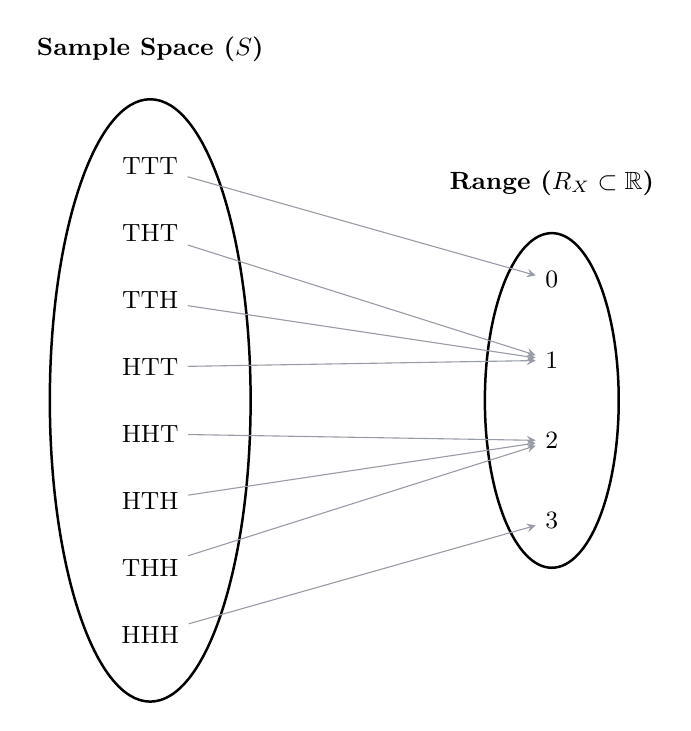
\begin{tikzpicture}[scale=0.85, >=stealth]
% Sample Space Ellipse
\draw[thick] (-3,0) ellipse (1.5 and 4.5);\node[above=10pt] at (-3,4.5) {\textbf{Sample Space ($S$)}};
% Outcomes in S
\node (ttt) at (-3,3.5) {TTT};
\node (tht) at (-3,2.5) {THT};
\node (tth) at (-3,1.5) {TTH};
\node (htt) at (-3,0.5) {HTT};
\node (hht) at (-3,-0.5) {HHT};
\node (hth) at (-3,-1.5) {HTH};
\node (thh) at (-3,-2.5) {THH};
\node (hhh) at (-3,-3.5) {HHH};

% Real Line / Range Ellipse
\draw[thick] (3,0) ellipse (1 and 2.5);
\node[above=10pt] at (3,2.5) {\textbf{Range ($R_X \subset \mathbb{R}$)}};

% Values in R_X
\node (v0) at (3,1.8) {0};
\node (v1) at (3,0.6) {1};
\node (v2) at (3,-0.6) {2};
\node (v3) at (3,-1.8) {3};

% Mappings (Arrows)
\draw[->, gray!70] (ttt) -- (v0);
\draw[->, gray!70] (tht) -- (v1);
\draw[->, gray!70] (tth) -- (v1);
\draw[->, gray!70] (htt) -- (v1);
\draw[->, gray!70] (hht) -- (v2);
\draw[->, gray!70] (hth) -- (v2);
\draw[->, gray!70] (thh) -- (v2);
\draw[->, gray!70] (hhh) -- (v3);
\end{tikzpicture}\caption{Mapping from the Sample Space to the Real Line for $X = \text{number of heads}$.}
\end{figure}
\end{example}



\begin{example}
In industrial monitoring, such as that performed by the Environmental Council of Zambia (ECZ), the nature of the data determines the classification of the variable.
\begin{enumerate}
\item Pesticide Concentration ($X$):If we measure the mass of pesticide in milligrams per liter, $X$ can take any value in a continuous interval. Then the range is  $$R_X = \{x \in \mathbb{R} : x \geq 0\},$$ and the data type is  continuous (uncountably infinite outcomes).
\item Monthly Compliance ($X$):If we count the number of months until a company fails an inspection, $X$ can be any whole number.The range is $$R_X = \{0, 1, 2, 3, \dots\},$$ and the data type is  discrete (countably infinite outcomes).
\end{enumerate}
\end{example}


\begin{note}
In practice, we use $X$ (uppercase) to refer to the name of the variable and $x$ (lowercase) to refer to a specific value it might take. 
\end{note}








\section{Discrete Random Variables}
\begin{definition}
A random variable $X$ is said to be discrete if its range $R_X$ is either finite or countably infinite. This means the possible values can be listed in a sequence $x_1, x_2, x_3, \dots$.
\end{definition}


\begin{definition}[\textbf{Probability Mass Function (PMF)}]
The probability distribution of a discrete random variable is described by a probability mass function, denoted as $f_X(x)$ or $P(X=x)$. This function assigns a probability to each possible value in the range of $X$ such that:
\begin{enumerate}
\item $f_X(x) \geq 0$ for all $x$.
\item $\sum_{x \in R_X} f(x) = 1$.
\end{enumerate}
\end{definition}




%ShutterstockExample 2.2.1: 
\begin{example}
Let the random variable $X$ represent the number of heads obtained in three independent tosses of a fair coin.
\begin{enumerate}
\item \textbf{Tabular Representation.} The distribution can be summarized in a probability table, which provides a clear view of the entire probability mass:
\begin{table}[H]
\centering\renewcommand{\arraystretch}{1.5}
\begin{tabular}{|c|c|c|c|c|}
\hline
$x$ & 0 & 1 & 2 & 3\\ 
\hline
$P(X=x)$ & $1/8$ & $3/8$ & $3/8$ & $1/8$\\ 
\hline
\end{tabular}
\caption{Probability distribution for the number of heads in 3 tosses.}
\end{table}

\item \textbf{Functional Representation (The Formula).} For a balanced coin, the probability of heads $p = 1/2$. The probability of observing exactly $x$ heads in 3 trials follows the Binomial logic:
$$\begin{aligned}
P(X=x) &= \binom{3}{x} \left( \frac{1}{2} \right)^x \left( \frac{1}{2} \right)^{3-x} \\
&= \binom{3}{x} \left(\frac{1}{2} \right)^3 \\
& = \frac{\binom{3}{x}}{8}, \quad x = 0, 1, 2, 3
\end{aligned}$$
\end{enumerate}
\end{example}



There are special discrete probability functions which do arise in many experiments and will discuss them later. There are Bernoulli, Binomial, Poisson, Geometric, Hypergeometric, discrete uniform e.te.c









\section{Continuous Random Variables}
\vspace{-15pt}

\begin{definition}
A random variable $X$ is continuous if its range $R_X$ is an uncountable interval (or a collection of intervals) of real numbers. $X$ can take on any value within a given range.
\end{definition}


\begin{definition}
For a continuous random variable, we define a probability density function, $f_X(x)$, such that:
\begin{enumerate}
\item $f_X(x) \geq 0$ for all $x \in \mathbb{R}$.
\item $\int_{-\infty}^{\infty} f_X(x) \, dx = 1$ (The total area under the curve is 1).
\end{enumerate}
\end{definition}




\begin{remark}
\begin{enumerate}
\item  For a continuous random variable, the probability of assuming any exact value is zero: $P(X = x) = 0$.
\item Because $P(X=x) = 0$, the inclusion or exclusion of endpoints in an interval does not change the probability:$$P(a < X < b) = P(a \leq X \leq b) = P(a \leq X < b) = P(a < X \leq b)$$
\item  Probability is found by integrating the p.d.f over the desired interval: $$P(a < X < b) = \int_{a}^{b} f_X(x) \, dx.$$
\end{enumerate}
\end{remark}



\begin{example}
Let $X$ be a random variable with the following p.d.f$$f_X(x) = \begin{cases} \frac{x+1}{8}, & 2 < x < 4 \\ 0, & \text{elsewhere} \end{cases}$$
\begin{figure}[H]
\centering
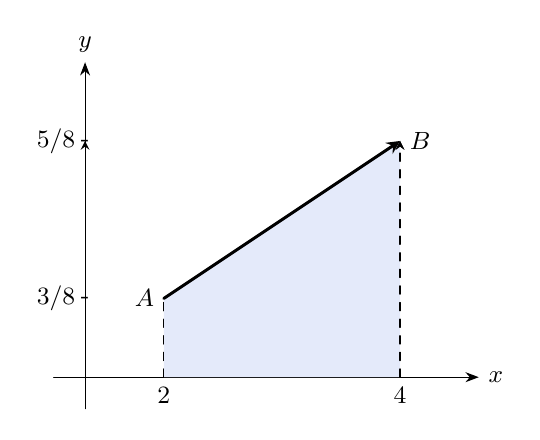
\begin{tikzpicture}[->,>=stealth]
\draw[-Stealth](-0.4,0)--(5,0)node[right]{$x$};
\draw[-Stealth](0,-0.4)--(0,4)node[above]{$y$};
\draw(1,0)node[below]{2}
%(3,0)node[below]{3}
(4,0)node[below]{4}
(0,1)node[]{-}
(0,3)node[]{-}
(0,1)node[left]{$3/8$}
(0,3)node[left]{$5/8$};
\path[fill=blue!12, dashed](1,0)--(1,1)--(4,3)--(4,0);
\draw[very thick](1,1)--(4,3);
\draw(1,1)node[left]{$A$}
(4,3)node[right]{$B$};
\draw[dashed](1,0)--(1,1)
(4,0)--(4,3);
\end{tikzpicture}
\caption{The c.d.f of $X$ rising from $3/8$ at $x=2$ to $5/8$ at $x=4$; the shaded area under the p.d.f is the probability accumulated between them.}
\end{figure}


\begin{enumerate}
\item[(i).] Show that $f(x)$ is probability density function.
\begin{proof}[\textbf{\textit{Solution}}]
$$\text{Area} = \int_{2}^{4} \frac{x+1}{8} \, dx = \left[ \frac{(x+1)^2}{16} \right]_{2}^{4} = \frac{(4+1)^2 - (2+1)^2}{16} = \frac{25-9}{16} = 1$$
\end{proof}


\item[(ii).] Find $P(X>3.5)$
\begin{proof}[\textbf{\textit{Solution}}]
$$P(X > 3.5) = \int_{3.5}^{4} \frac{x+1}{8} \, dx = \left[ \frac{(x+1)^2}{16} \right]_{3.5}^{4} = \frac{5^2 - 4.5^2}{16} = \frac{25 - 20.25}{16} = \frac{4.75}{16}.$$
\end{proof}



\item[(iii).] Find $P(2.4<X<3.5)$
\begin{proof}[\textbf{\textit{Solution}}]
$$P(2.4 < X < 3.5) = \int_{2.4}^{3.5} \frac{x+1}{8} \, dx = \left[ \frac{(x+1)^2}{16} \right]_{2.4}^{3.5} = \frac{4.5^2 - 3.4^2}{16} =  \approx 0.5431$$
\end{proof}
\end{enumerate}
\end{example}


\begin{table}[H]
\centering
\renewcommand{\arraystretch}{2} % Increases row height for better readability
\begin{tabular}{|l|c|c|}
\hline
\textbf{Property} & \textbf{Discrete Random Variable} & \textbf{Continuous Random Variable} \\ \hline
\textbf{Support ($R_X$)} & Finite or Countably Infinite & Uncountable Interval(s) \\ \hline
\textbf{Function Type} & Probability Mass Function (PMF) & Probability Density Function (PDF) \\ \hline
\textbf{Notation} & $f(x) = P(X = x)$ & $f(x)$ (where $P(X=x) = 0$) \\ \hline
\textbf{Conditions} & $0 \leq f(x) \leq 1$ & $f(x) \geq 0$ \\ \hline
\textbf{Total Value} & $\sum_{x \in R_X} f(x) = 1$ & $\int_{-\infty}^{\infty} f(x) dx = 1$ \\ \hline
\textbf{Interval Prob.} & $P(a \le X \le b) = \sum_{x=a}^{b} f(x)$ & $P(a \le X \le b) = \int_{a}^{b} f(x) dx$ \\ \hline
\end{tabular}
\caption{Side-by-side comparison of Discrete and Continuous frameworks.}
\end{table}


\begin{figure}[H]
\centering
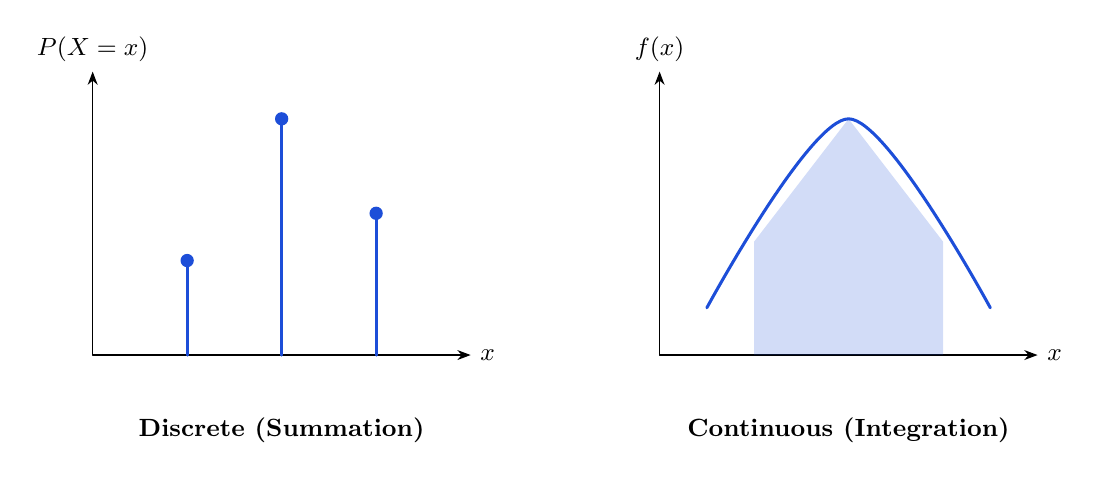
\begin{tikzpicture}[scale=1.2]
    % Discrete Side
    \begin{scope}[shift={(0,0)}]
        \draw[->] (0,0) -- (4,0) node[right] {$x$};
        \draw[->] (0,0) -- (0,3) node[above] {$P(X=x)$};
        \foreach \x/\h in {1/1, 2/2.5, 3/1.5} {
            \draw[very thick, blue] (\x,0) -- (\x,\h);
            \fill[blue] (\x,\h) circle (2pt);
        }
        \node at (2,-0.8) {\textbf{Discrete (Summation)}};
    \end{scope}

    % Continuous Side
    \begin{scope}[shift={(6,0)}]
        \draw[->] (0,0) -- (4,0) node[right] {$x$};
        \draw[->] (0,0) -- (0,3) node[above] {$f(x)$};
        \draw[very thick, blue, smooth] plot coordinates {(0.5,0.5) (2,2.5) (3.5,0.5)};
        \fill[blue, opacity=0.2] plot coordinates {(1,0) (1,1.2) (2,2.5) (3,1.2) (3,0)} -- cycle;
        \node at (2,-0.8) {\textbf{Continuous (Integration)}};
    \end{scope}
\end{tikzpicture}
\caption{Visualizing the transition from individual points of mass to a density of area.}
\end{figure}








\section{Mathematical Expectations and Generating Functions of Random Variables}
While the p.m.f and p.d.f provide a complete description of a random variable, we often require concise numerical descriptors to summarize a distribution's location and spread. This section moves from basic Expectations to the powerful ``transform'' methods—Generating Functions—which serve as essential tools for identifying distributions and simplifying the calculation of higher-order moments.

\subsection{Expectations and Moments}
\vspace{-8pt}
\begin{definition}
Let $X$ be a random variable the mean or expectation of the random variable $X$ denoted by $\mu$ or $E(X)$ and it's given by
\[ E(X)=
\begin{cases}
\sum\limits_{\text{all}\, x}xf_X(x)=\sum\limits_{\text{all}\, x}xP(X=x), & \text{if}\quad X\quad\text{is discrete.}\\\\
\int\limits_{\text{all}\,x}xf_X(x)\, dx, &\text{if}\quad X\quad \text{is continuous}\\
\end{cases}
\]
\end{definition}





\begin{example}
Suppose we toss a fair coin three times. Let the random variable $X$ represent the number of heads obtained. The probability mass function (PMF) of $X$ is given by:$$f_X(x) = P(X = x) = \frac{\binom{3}{x}}{8}, \quad \text{for } x \in \{0, 1, 2, 3\}$$ Find the expected value of $X$.
\end{example}

\begin{proof}[\textbf{\textit{Solution}}]
The expected value is 
$$\begin{aligned}
E(X) & = \sum_{x} x \cdot f_X(x)\\
&= \sum_{x=0}^{3} x \cdot \frac{\binom{3}{x}}{8} \\
&= \frac{1}{8} \left[ \sum_{x=0}^{3} x \cdot \binom{3}{x} \right] \\
&= \frac{1}{8} \left[ 0 \cdot \binom{3}{0} + 1 \cdot \binom{3}{1} + 2 \cdot \binom{3}{2} + 3 \cdot \binom{3}{3} \right] \\
&= \frac{1}{8} \left[ 0(1) + 1(3) + 2(3) + 3(1) \right] \\
&= \frac{3 + 6 + 3}{8} = \frac{12}{8} \\
\mathbf{E(X)} &\mathbf{= 1.5}
\end{aligned}$$
\textit{Interpretation:} If we were to repeat this experiment many times, we would expect to see an average of 1.5 heads per three tosses. Note that while the outcome $1.5$ is not possible in a single trial, it represents the long-run theoretical mean.
\end{proof}


\begin{figure}[H]
\centering
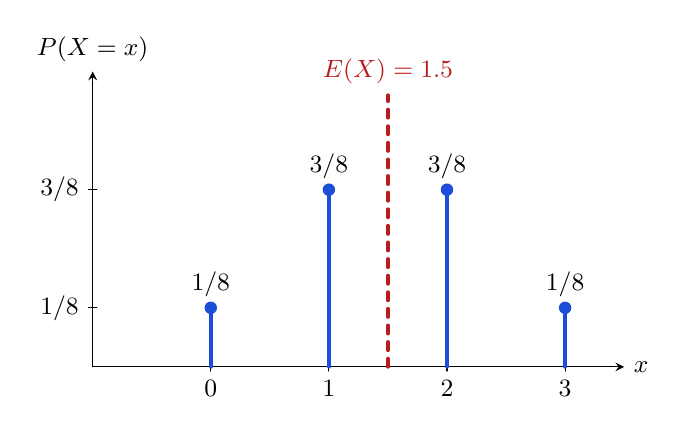
\begin{tikzpicture}[scale=1.5, >=stealth]
    % Axes
    \draw[->] (0,0) -- (4.5,0) node[right] {$x$};
    \draw[->] (0,0) -- (0,2.5) node[above] {$P(X=x)$};

    % X-axis labels
    \foreach \x in {0,1,2,3}
        \draw (\x+1,1pt) -- (\x+1,-1pt) node[below] {\x};

    % Y-axis labels
    \draw (1pt,0.5) -- (-1pt,0.5) node[left] {$1/8$};
    \draw (1pt,1.5) -- (-1pt,1.5) node[left] {$3/8$};

    % Probability Bars (Masses)
    % Height 0.5 represents 1/8, Height 1.5 represents 3/8
    \draw[ultra thick, blue] (1,0) -- (1,0.5) node[above, black] {\small $1/8$};
    \draw[ultra thick, blue] (2,0) -- (2,1.5) node[above, black] {\small $3/8$};
    \draw[ultra thick, blue] (3,0) -- (3,1.5) node[above, black] {\small $3/8$};
    \draw[ultra thick, blue] (4,0) -- (4,0.5) node[above, black] {\small $1/8$};
    
    % Optional: dots on top of the bars
    \fill[blue] (1,0.5) circle (1.5pt);
    \fill[blue] (2,1.5) circle (1.5pt);
    \fill[blue] (3,1.5) circle (1.5pt);
    \fill[blue] (4,0.5) circle (1.5pt);

    % Mean indicator
    \draw[dashed, red, ultra thick] (2.5,0) -- (2.5,2.3) node[above] {$E(X)=1.5$};
\end{tikzpicture}
\caption{PMF for the number of heads in 3 tosses, showing the mean at the center of symmetry.}
\end{figure}





\begin{example}
Let $X$ be a continuous random variable with the probability density function (pdf) defined by:
$$f_X(x) =
\begin{cases}
\dfrac{x+1}{8}, & 2 < x < 4 \\
0, & \text{otherwise}
\end{cases}$$Calculating the Expected Value $E(X)$.
\end{example}

\begin{proof}[\textbf{\textit{Solution}}]
$$\begin{aligned}
E(X) & = \int_{-\infty}^{\infty} x \cdot f_X(x) \, dx\\
&= \int_{2}^{4} x \left(\frac{x+1}{8} \right) dx \\
&= \frac{1}{8} \int_{2}^{4} (x^2 + x) , dx \\
&= \frac{1}{8} \left[\frac{x^3}{3} + \frac{x^2}{2} \right]_{2}^{4} \\
&= \frac{1}{8} \left[ \left(\frac{64}{3} + 8 \right) - \left( \frac{8}{3} + 2 \right) \right] \\
&= \frac{1}{8} \left[ \frac{56}{3} + 6 \right] = \frac{1}{8} \left[ \frac{56 + 18}{3} \right] \\
&= \frac{74}{24} \\
& = \frac{37}{12}
\end{aligned}$$
\end{proof}

\begin{figure}[H]
\centering
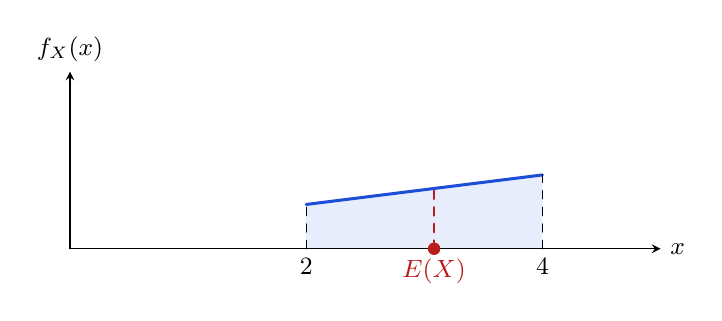
\begin{tikzpicture}[scale=1.5, >=stealth]
    % Axes
    \draw[->] (0,0) -- (5,0) node[right] {$x$};
    \draw[->] (0,0) -- (0,1.5) node[above] {$f_X(x)$};

    % Plotting the PDF line
    % at x=2, y=3/8 (0.375). at x=4, y=5/8 (0.625)
    \draw[very thick, blue] (2,0.375) -- (4,0.625);
    \draw[dashed] (2,0) -- (2,0.375);
    \draw[dashed] (4,0) -- (4,0.625);
    
    % Shading the area
    \fill[blue, opacity=0.1] (2,0) -- (2,0.375) -- (4,0.625) -- (4,0) -- cycle;

    % X-axis labels
    \node[below] at (2,0) {2};
    \node[below] at (4,0) {4};

    % Mean indicator
    \draw[red, thick, dashed] (3.083, 0) -- (3.083, 0.51);
    \fill[red] (3.083,0) circle (1.5pt) node[below] {\small $E(X)$};
\end{tikzpicture}
\caption{The PDF of $X$ over the interval $(2,4)$. The mean is located at $x \approx 3.083$.}
\end{figure}



\begin{thm}
Let $X$ be a random variable with probability function $f_X(x)$, and $g(x)$ be any function then the expectation  of $h(x)$ is given by
\[ E(g(x))=
\begin{cases}
\sum\limits_xh(x)f_X(x), & \text{if}\quad X\quad \text{is discrete}\\\\
\int\limits_xh(x)f_X(x), &\text{if}\quad X\quad\text{is continuous}\\
\end{cases}
\]
\end{thm}



\begin{remark}
If $h(x)=x$ which is the identity function $E[h(x)]=E(x)=\mu$.
\end{remark}


\begin{thm}[\textbf{Properties of Expectations}]
Let $X$ be a random variable, $b$ and $c$ be constants, $g(x)$ and $h(x)$ be functions, then
\begin{enumerate}
\item[(i).] $E[b\, g(X)+c\, h(X)]=b\,E[g(X)] +c\,E[h(X)]$
\item[(ii).] $E[g(X) + b] =  E[g(X)] + b$
\begin{proof}
Suppose that $X$ is a continuous random variable, then 
\begin{align*}
E[g(X)  + b] & = \int^{\infty}_{-\infty} [g(X) + b]\, f_X(x)\, dx \\
& = \int^{\infty}_{-\infty}g(X)\, f_X(x)\, dx + \int^{\infty}_{-\infty} b\, f_X(x)\, dx\\
& = E[g(X)] + b\int^{\infty}_{-\infty} f_X(x)\, dx\\
& = E[g(X)] + b.
\end{align*}
This completes the proof.
\end{proof}


\item[(iii).] If $g(X)\leq h(X)$, then $E(g(X))\leq E(h(X))$
\begin{proof}
Let $g(x)=a$ and $h(x)=b$, where $a<b$.
\begin{align*}
E[g(X)] &=E(a)=a\\
E[h(X)] &=E(b)=b 
\end{align*}
Therefore,  $a<b \,\,\implies\,\, E[g(X)] < E[h(X)].$
\end{proof}
\item[(iv).] $E[E(X)] = E(X)$
\end{enumerate}
\end{thm}




\begin{remark}[\textbf{Special Expectations}]
If $X$ is a random variable, then
\begin{enumerate}
\item The $k^{\text{th}}$ moment (about the origin): \[E(X^{k})\]
\item The $k^{\text{th}}$ moment about the mean: \[E\left[(X - \mu)^k\right].\]
\item The $k^{\text{th}}$ factorial moment: \[E\left[X^{(k)}\right]= E\left[X(X-1)(X-2)\, \cdots\, (X - k + 1)\right]\]
\end{enumerate}
\end{remark}




\begin{definition}
Let $X$ be a random variable with mean $\mu$, then then variance of $X$ denoted by $\sigma^2$ or Var$(X)$ is given by $$\sigma^2=E(X-\mu)^2,$$ where  $\mu=E(X)$, \,\, $\sigma^2>0$.
\end{definition}



Computation formula of $\sigma^2$ is given by 
\begin{align*}
\sigma^2 &=E(X-\mu)^2\\
& =E[X-E(X)]^2\\
&=E[X^2-2XE(X)+E(X)^2]\\
&=E(X^2)-E[2XE(X)]+E[E(X)]^2\\
&=E(X^2)-2E(X)E(X)+[E(X))]^2\\
&=E(X^2)-2[E(X)]^2+[E(X)]^2\\
&=E(X^2)-[E(X)]^2.
\end{align*}



\begin{example}
Using \textit{Example 2.4.2}, we found the mean $E(X) = 1.5$. Now we find the variance \[\operatorname{Var}(X) = E(X^2) - E[E(X)]^2.\] First we find $E(X^2)$.
$$\begin{aligned}
E(X^2) & = \sum_x x^2\cdot f_X(x)\\
 &= \sum_{x=0}^{3} x^2 \cdot \frac{\binom{3}{x}}{8} \\
&= \frac{1}{8} \left[ 0^2\binom{3}{0} + 1^2\binom{3}{1} + 2^2\binom{3}{2} + 3^2\binom{3}{3} \right] \\
&= \frac{1}{8} \left[ 0(1) + 1(3) + 4(3) + 9(1) \right] \\
&= \frac{24}{8}\\
& = 3.
\end{aligned}$$

Now, substitute $E(X^2) = 3$ and $E(X) = 1.5$  into the variance formula:
$$\begin{aligned}
\operatorname{Var}(X) &= E(X^2) - [E(X)]^2 \\
&= 3 - (1.5)^2 \\
&= 3 - 2.25 \\
&= 0.75
\end{aligned}$$
\end{example}



\begin{example}
In \textit{Example 2.4.3} we calculated the mean to be $E(X) = \frac{37}{12}$. Now, we find $E(X^2)$ and subsequently the variance.
$$\begin{aligned}
E(X^2) &= \int_{2}^{4} x^2 \left( \frac{x+1}{8} \right) dx \\
&= \frac{1}{8} \int_{2}^{4} (x^3 + x^2) \, dx \\
&= \frac{1}{8} \left[ \frac{x^4}{4} + \frac{x^3}{3} \right]_{2}^{4} \\
&= \frac{1}{8} \left[ \left( \frac{256}{4} + \frac{64}{3} \right) - \left( \frac{16}{4} + \frac{8}{3} \right) \right] \\
& = \frac{236}{24}
 = \frac{59}{6}
\end{aligned}$$
Now, we substitute $E(X^2) = \frac{59}{6}$ and $E(X) = \frac{37}{12}$ into the variance formula:
$$\begin{aligned}
\operatorname{Var}(X) &= E(X^2) - [E(X)]^2 \\
&= \frac{59}{6} - \left( \frac{37}{12} \right)^2 \\
&= \frac{59}{6} - \frac{1369}{144} \\
&= \frac{59 \times 24}{144} - \frac{1369}{144} \\
&= \frac{1416 - 1369}{144} \\
& = \frac{47}{144}.
\end{aligned}$$
\end{example}


\begin{thm}
If $X$ is a random variable with mean $\mu$ and variance $\sigma^2$, then \[\operatorname{Var}(aX + b) = a^2 \, \operatorname{Var}(X),\] where $a$ and $b$ are any real constants.
\end{thm}


\begin{proof}
\begin{align*}
\operatorname{Var}(aX + b) & = E\left([(aX + b) - \mu_{aX + b}]^2\right)\\
& = E\left([(aX + b) - E(aX + b)]^2\right)\\
& = E\left([aX + b - aE(X) - b]^2\right)\\
& = E\left([aX - aE(X)]^2\right)\\
& = E\left(a^2 [X - E(X)]^2\right)\\
& = a^2E\left([X-\mu]^2\right)\\
& = a^2\, \operatorname{Var}(X).
\end{align*}
\end{proof}



\begin{remark}
\begin{enumerate}
\item The mean is the balance point (the center of gravity) where the seesaw stays level. while, the variance describes how the weight is spread out. In physics, this is called the moment of inertia.
\item Th square root of the Var$(X)$ is called the \textit{standard deviation} of $X$, that is \[\sigma_X = \sqrt{\text{Var}(X)}.\]
\end{enumerate}
\end{remark}




\begin{exe}
Let $X$ have the p.d.f \[f_X(x) = \begin{cases}
\frac{2x}{k^2}, & 0\leq x \leq k\\
0, & \text{otherwise}.
\end{cases}\] For what value of $k$ is the variance of $X$ equal to 2?
\end{exe}
%%%%%%%%%%%%%%%%%%%%%%%%%%%%%%%%%%%%%%%%%%%%%%%%%%%%%%%%%%%%%%%%%%%%%%%%%%%%%%%%%%%%%%%%%%%%%%%%%%



\subsection{Probability Generating Functions (PGFs)}
For discrete random variables taking non-negative integer values, the PGF acts as a powerful ``storage device'' where the individual probabilities of the distribution are encoded as the coefficients of a power series.

\begin{definition}
For a discrete random variable $X$, the PGF, denoted by $G_X(t)$, is defined as $$G_X(t) = E(t^X) = \sum_{x=0}^{\infty} t^x P(X=x)$$ for all values of $t \in \mathbb{R}$ for which the power series converges.
\end{definition}



\begin{remark}
The three key properties of PGF include:
\begin{enumerate}
\item  Evaluating the PGF at $t=1$ must always equal 1, as it represents the sum of all probabilities in the sample space:$$G_X(1) = \sum_{x=0}^{\infty} P(X=x) = 1$$
\item The individual probabilities can be recovered by taking the $k$-th derivative of the PGF and evaluating it at $t=0$:
\[P(X=k) = \frac{G_X^{(k)}(0)}{k!}\]

\item The derivatives of the PGF evaluated at $t=1$ generate what is call \textit{factorial moments}. The first derivative gives the mean:
\[G_X'(1) = E(X)\]
The second derivative provides the second factorial moment, which is used to calculate variance:
\[G_X''(1) = E[X(X - 1)] = E(X^2) - E(X).\]
Therefore \[\operatorname{Var}(X) = G''_X(1) + G'_X(1) - [G'_X(1)]^2.\]
\end{enumerate}
\end{remark}







\begin{example}
Consider the following discrete probability distribution
\begin{table}[H]
\centering
\begin{tabular}{|c|c|c|c|c|}
\hline
$x$ & 2 & 4 & 5 & 10 \\ 
\hline
$P(X=x)$ & 0.1 & 0.2 & 0.3 & 0.4 \\ 
\hline
\end{tabular}
\end{table}
Find the Probability Generating Function, $G_X(t)$.
\end{example}

\begin{proof}[\textbf{\textit{Solution}}]
By definition, the PGF is the expected value of $t^X$
\begin{align*}
G_X(t) & = \sum_{x} t^x P(X=x) \\
& = t^2 P(X=2) + t^4 P(X=4) + t^5 P(X=5) + t^{10} P(X=10) \\
&= 0.1t^2 + 0.2t^4 + 0.3t^5 + 0.4t^{10}
\end{align*}
\end{proof}




\begin{example}
In a game, the probability that $A$ wins on her $x$th go can can be described as a discrete random variable $X$, with probability function \[P(X = x) = \frac{1}{2^x}\,,\quad \text{for}\,\, x = 1,2, 3, 4, \cdots\]
\begin{enumerate}
\item Find the probability generating function.
\begin{proof}[\textbf{\textit{Solution}}]
Note that \[P(X = 1)  = \frac{1}{2}, \quad P(X = 2) = \frac{1}{2^2}, \quad P(X = 3) = \frac{1}{2^3}, \quad P(X = 4) = \frac{1}{2^4}, \quad \cdots\]
\begin{align*}
G_X(t) & = \sum_x t^x P(X = x)\\
& = \frac{1}{2}t + \frac{1}{2^2}t^2 + \frac{1}{2^3}t^3 + \frac{1}{2^2}t^4+ \cdots\\
& = \sum^{\infty}_{x = 1}\left(\frac{t}{2}\right)^x
\end{align*}


Note that the ``standard geometric series'' is usually presented as:$$\sum_{n=0}^{\infty} r^n = \frac{1}{1-r}$$However, if you start at $n=1$, you are simply missing the first term ($r^0 = 1$):$$\sum_{n=1}^{\infty} r^n = \left(\sum_{n=0}^{\infty} r^n\right) - 1 = \frac{1}{1-r} - 1 = \frac{r}{1-r}.$$

Thus, the closed-form PGF is $$G_X(t) = \frac{\frac{t}{2}}{1 - \frac{t}{2}} = \frac{t}{2-t}, \quad \text{for } |t| < 2.$$
\end{proof}


\item Find $E(X)$ and $\operatorname{Var}(X)$.

\begin{proof}[\textbf{\textit{Solution}}]
The mean $E(X)$, $$G_X'(t) = \frac{(2-t)(1) - t(-1)}{(2-t)^2} = \frac{2-t+t}{(2-t)^2} = \frac{2}{(2-t)^2}$$Evaluating at $t=1$, $$E(X) = G_X'(1) = \frac{2}{(2-1)^2} = 2.$$

The variance $\text{Var}(X)$.  $G_X''(1)$:$$G_X''(t) = \frac{d}{dt} [2(2-t)^{-2}] = 2(-2)(2-t)^{-3}(-1) = \frac{4}{(2-t)^3}$$ Evaluating at $t=1$, $$G_X''(1) = \frac{4}{(2-1)^3} = 4$$

Now, use the variance formula for PGFs. $$\text{Var}(X) = G_X''(1) + G_X'(1) - [G_X'(1)]^2$$$$\text{Var}(X) = 4 + 2 - (2)^2 = 6 - 4$$ $$\text{Var}(X) = 2.$$
\end{proof}
\end{enumerate}
\end{example}






%%%%%%%%%%%%%%%%%%%%%%%%%%%%%%%%%%%%%%%%%%%%%%%%%%%%%%%%%%%%%%%%%%%%%%%%%%%%%%%%%%%%%%%%%%%%%%%
\subsection{Moment Generating Functions (MGFs)}
There are some distributions whose moments are difficult to compute from the definition. A moment generating function is a real valued function from which one can generate all the moments of a given random variable. 



\begin{definition}[\textbf{Moment Generating function (m.g.f)}]
Let $X$ be a random variable with probability function $f_X(x)$ then the moment generating function of $X$ is denoted by $M_X(t)$ and given by $M_X(t)=E(e^{tx})$.
\[ M_X(t)=
\begin{cases}
\sum\limits_xe^{tx}P(X=x),&\text{if}\hspace{0.3cm} X\hspace{0.3cm} \text{is discrete}\\\\
\int\limits_xe^{tx}f_X(x)dx &\text{if}\hspace{0.3cm}X\hspace{0.3cm} \text{is continuous}\\
\end{cases}
\]
\end{definition}

The exponential series
$$e^y  =\sum^{\infty}_{k=0}\frac{y^k}{k!} =1+y+\frac{y^2}{2!}+\frac{y^3}{3!}+\cdots$$
If $\, y = 1$, 
\[e=1+1+\frac{1}{2}+\frac{1}{3!}+\frac{1}{4!}+\cdots\]




\begin{remark}
\begin{enumerate}
\item[(a).] We only need $M_X(t)$ to be defined in the neighbourhood of zero  i.e $t\in (-\varepsilon,\varepsilon)$ for any $\varepsilon >0$.
\item[(b).] Not every random variable has a moment generating function. But if the moment generating function of a random variable exists, then it is unique.
\item[(c).] The m.g.f is used to generate moments i.e $E(X^k)$ is known as the $k^{\text{th}}$ raw moment.
% Was \frac{d}{dX}: the m.g.f. is differentiated with respect to t, not X.
\[E(X)  =\frac{d}{dt}M_X(t)\Bigg|_{t=0}\]

% Was d^^2, which is a LaTeX escape sequence, not a squared d - it broke the
% whole display and MathJax printed the raw source.
\[E(X^2) =\frac{d}{dt}\left[\frac{d}{dt}M_X(t)\right]_{t=0} \, =\, \frac{d^2}{dt^2}M_X(t)\Bigg|_{t=0}\]

\[\sigma^2  =E(X^2)-(E(X))^2.\]
\end{enumerate}
\end{remark}


\begin{example}
What is the moment generating function of the random variable $X$ whose p.d.f is given by \[f_X(x) = e^{-x}\, \, \quad x > 0.\] What are the mean and variance of $X$?
\end{example}

\begin{proof}[\textbf{\textit{Solution.}}]
The moment generating function of $X$ is 
\begin{align*}
M_X(t) & = E(e^{tX})\\
& = \int^{\infty}_0 e^{tx}\, e^{-x}\, dx\\
& = \int^{\infty}_0e^{-(1-t)}\, dx\\
& = \frac{1}{1-t}\left[-e^{-(1-t)x}\right]^{\infty}_0\\
& = \frac{1}{1-t}\, ,\quad 1 - t > 0.
\end{align*}
The expected value of $X$ is
\begin{align*}
E(X) & = \frac{d}{dt}\, M_X(t)\Bigg|_{t = 0}\\
& = (-1)(-1)(1-t)^{-2}\Big|_{t =0}\\
& = \frac{1}{(1-t)^2}\Bigg|_{t = 0}\\
& = 1.
\end{align*}
Similarly
\begin{align*}
E(X^2) & = \frac{d^2}{dt^2}\, M(t)\Bigg|_{t = 0}\\
& = \frac{(-1)(-2)}{(1 - t)^3}\Bigg|_{t = 0}\\
& = \frac{2}{(1 - t)^3}\Bigg|_{t = 0}\\
& = 2.
\end{align*}
Hence, the variance of $X$ is \[\operatorname{Var}(X) = E(X^2) - [E(X)]^2 = 2 - 1 = 1.\]
\end{proof}




\begin{thm}
Let $M_X(t)$ be the moment generating function of the random variable $X$. If \begin{equation}\label{eq:mgf-taylor}
M_X(t) = a_0 + a_1t + a_2t^2 +\, \cdots\, a_nt^n + \, \cdots
\end{equation}
is the Taylor series expansion of $M_X(t)$, then \[E(X^n) = (n!)\, a_n\] for $n \in \mathbb{R}$.
\end{thm}
\begin{proof}
Let $M_X(t)$ be the m.g.f. of the random variable $X$. The Taylor series expansion of $M_X(t)$ about zero is given by \[M_X(t) = M(0) + \frac{M'(0)}{1!}t + \frac{M''(0)}{2!}t^2+ \frac{M'''(0)}{3!}t^3 + \cdots + \frac{M^{(n)}(0)}{n!}t^n+ \cdots\]
Since $\, E(X^n) = M^{(n)}(0)\,$ for $n\geq 1$ and $M(0) = 1$, we have 
\begin{equation}\label{eq:mgf-moments}
M(t) = 1 + \frac{E(X)}{1!}t + \frac{E(X^2)}{2!}t^2 + \frac{E(X^3)}{3!}t^3 + \cdots + \frac{E(X^n)}{n!}t^n + \cdots
\end{equation}
% Was hardcoded as "(2.1) and (2.2)", which did not match the numbers the
% equations actually carry. Labels keep the reference correct as content moves.
Comparing \eqref{eq:mgf-taylor} and \eqref{eq:mgf-moments}, equating the coefficients of the like powers of $t$, we obtain \[a_n = \frac{E(X^n)}{n!}\, \implies \, E(X^n) = (n!)\, a_n.\] Hence the proof.
\end{proof}




\begin{example}
Find the 99$^{\text{th}}$ moment of $X$ about the origin, if the moment generating function of $X$ is $M_X(t) = \frac{1}{1 + t}$?
\end{example}
\begin{proof}[\textbf{\textit{Solution}}]
The Taylor series expansion of $M_X(t)$ is
\begin{align*}
M_X(t) & = \frac{1}{1+t}
 = \frac{1}{1 - (-t)}\\
& = 1 + (-t) + (-t)^2 + (-t)^3  + \cdots + (-t)^n+ \cdots\\
& = 1 - t + t^2 - t^3 + \cdots + (-1)^nt^n + \cdots
\end{align*}
Therefore, $a_n = (-1)^n$ and we get $a_{99} = -1$. Thus, \[E(X^{99}) = (99!)a_{99} = -99!\]
\end{proof}




\subsection{Characteristic Functions}
\begin{definition}
If a random variable does not have a well-defined moment generating function m.g.f, we can use the \textit{characteristic function} as \[\phi_X(t) = E\left[e^{itX}\right],\] where $i = \sqrt{-1}$ and $t$ is a real number.
\end{definition}




\begin{thm}
Some of the properties of the characteristic function include
\begin{enumerate}
\item $\phi_X(t)$ is defined for all $t\in \mathbb{R}.$
\item $\left|\phi_X(t)\right| \leq \phi_X(0) = 1.$
\begin{proof}
Since $\left|e^{itX}\right| = 1$, then 
\[\left|\phi_X(t)\right|   = \left|E\left[e^{itX}\right]\right|  \leq E\left[\left|e^{itX}\right|\right] \leq 1.\]
\end{proof}
\item If the $n^{\text{th}}$ moment $E(X^n)$ exits, it can be found by differentiating the function $k$ times at the origin: \[E(X^n) = \frac{1}{i^n}\left[\frac{d^n}{dt^n}\phi_X(t)\right]_{t = 0}.\]
\item If you shift or scale a random variable (e.g., $Y = aX + b$), then \[\phi_{aX + b}(t) = e^{itb}\, \phi_X(at).\]
\end{enumerate}
\end{thm}



\begin{example}
Let $X$ be a random variable with a p.d.f $$f_X(x) = \lambda\, e^{-\lambda x}, \quad x > 0.$$ Use the characteristic function to find the mean.
\end{example}

\begin{proof}[\textbf{\textit{Solution}}]
Derive the characteristic function
\begin{align*}
\phi_X(t) & = E\left[e^{itX}\right]\\
& = \int_0^{\infty}e^{itx}\, \lambda e^{-\lambda x}\, dx\\
& = \lambda \int^{\infty}_0 e^{-(\lambda - it)x}\, dx\\
& = \lambda \left[-\frac{e^{-(\lambda - it)}}{(\lambda - it)}\right]^{\infty}_0\\
& = \frac{\lambda}{\lambda - it}.
\end{align*}
Then first derivative $(n = 1)$
\[\phi'_X(t) = \lambda (-1)(-i)(\lambda - it)^{-2} = \frac{i\lambda}{(\lambda - it)^2}.\]
The mean
\[E(X)  = \frac{1}{i}\, \phi'_X(0) = \frac{1}{i}\left(\frac{i\lambda}{\lambda^2}\right) = \frac{1}{\lambda}.\]
\end{proof}








%%%%%%%%%%%%%%%%%%%%%%%%%%%%%%%%%%%%%%%%%%%%%%%%%%%%%%%%%%%%%%%%%%%%%%%%%%%%%%%%%%%%%%%%%
\section{Some Important Discrete Probability Mass Function}
We focus on specific families of discrete random variables that appear frequently in scientific research, engineering, and economics. Each distribution is defined by one or more parameters that determine its shape and characteristics. By identifying a situation as fitting one of these models, we can use pre-derived formulas for their mean, variance, and generating functions.


\subsection{The Bernoulli Distribution}
The Bernoulli trial is the simplest form of a random experiment, characterized by exactly two possible outcomes: ``success'' and ``failure.'' By convention, we map the outcome ``success'' to the value $1$ and ``failure'' to the value $0$. Let $p$ denote the probability of success, where $0 \le p \le 1$. It follows that the probability of failure is $1-p$, often denoted as $q$.

\begin{definition}
A random variable $X$ is said to follow a Bernoulli distribution, denoted $X \sim \operatorname{Ber}(p)$, if its probability mass function (PMF) is:$$ f(x; p) = p^x(1-p)^{1-x}, \quad x \in {0, 1} $$where $p = P(X=1)$.
\end{definition}



\begin{figure}[H]
    \centering
    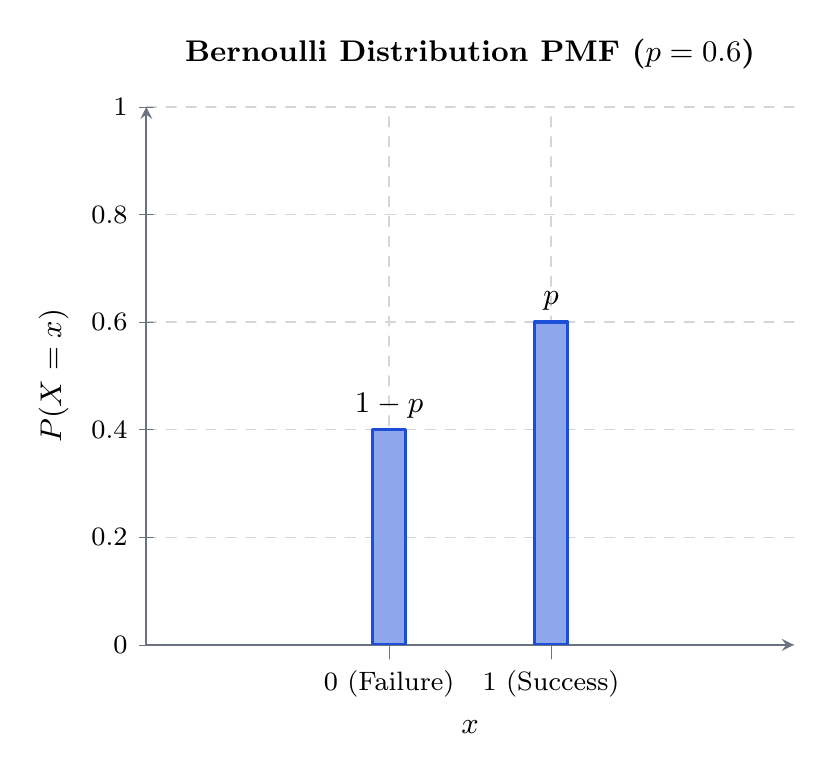
\begin{tikzpicture}[scale = 1.2]
        \begin{axis}[
            title={Bernoulli Distribution PMF ($p=0.6$)},
            xlabel={$x$},
            ylabel={$P(X=x)$},
            xmin=-0.5, xmax=1.5,
            ymin=0, ymax=1,
            xtick={0, 1},
            xticklabels={0 (Failure), 1 (Success)},
            ytick={0, 0.2, 0.4, 0.6, 0.8, 1.0},
            grid=major,
            grid style={dashed, gray!30},
            axis lines=left,
            enlarge x limits=0.5,
            ybar, % Uses bars to show the mass
            bar width=10pt
        ]
            
            % Data for p = 0.6
            % q = 0.4, p = 0.6
            \addplot[fill=blue!50, draw=blue] coordinates {(0, 0.4) (1, 0.6)};
            
            % Add labels on top of bars
            \node[above] at (axis cs:0, 0.4) {$1-p$};
            \node[above] at (axis cs:1, 0.6) {$p$};
            
        \end{axis}
    \end{tikzpicture}
    \caption{Probability Mass Function of a Bernoulli trial where $p=0.6$.}
\end{figure}




\begin{example}
Consider the experiment of rolling a fair six-sided die. What is the probability of obtaining a score of at least 5?
\end{example}

\begin{proof}[\textbf{Solution}]
The sample space is $S = \{1, 2, 3, 4, 5, 6\}$. We can define a Bernoulli trial by partitioning this set into:
\begin{itemize}
\item \textbf{Success ($X=1$):} The outcome is in the set $\{5, 6\}$.
\item \textbf{Failure ($X=0$):} The outcome is in the set $\{1, 2, 3, 4\}$.
\end{itemize}
Since the die is fair, the probability of success is:$$ p = P(X=1) = \frac{2}{6} = \frac{1}{3} $$Thus, the probability of rolling a score of at least 5 is $1/3$.
\end{proof}




\begin{thm}
If $X \sim \operatorname{Ber}(p)$, then:
\begin{enumerate}
\item \textbf{Mean:} $E(X) = p$.
\begin{proof}
By the definition of expectation:$$ E(X) = \sum_{x=0}^{1} x \cdot f(x; p) = (0)(1-p) + (1)(p) = p. $$
\end{proof}

\item \textbf{Variance:} $\operatorname{Var}(X) = p(1-p)$.
\begin{proof}
First, we calculate the second raw moment:
\[ E(X^2) = \sum_{x=0}^{1} x^2 \cdot f(x; p) = (0^2)(1-p) + (1^2)(p) = p. \]
Using the identity $\operatorname{Var}(X) = E(X^2) - [E(X)]^2$:
\[ \operatorname{Var}(X) = p - p^2 = p(1-p). \]
\end{proof}
\end{enumerate}
\end{thm}




\begin{thm}
The generating functions for $X \sim \operatorname{Ber}(p)$ are given by:
\begin{enumerate}
\item Probability Generating Function (PGF): $$ G_X(t) = E[t^X] = t^0(1-p) + t^1(p) = (1-p) + pt. $$
\item Moment Generating Function (MGF):
\[ M_X(t) = E[e^{tX}] = e^{0}(1-p) + e^{t}(p) = (1-p) + pe^t, \quad t \in \mathbb{R}. \]
\item Characteristic Function:
\[ \phi_X(t) = E[e^{itX}] = (1-p) + pe^{it}, \quad t \in \mathbb{R}. \]
\end{enumerate}\end{thm}










\subsection{Discrete Uniform}
The Discrete Uniform distribution describes a situation where a finite number of outcomes are all equally likely to occur. A classic example is the roll of a fair $N$-sided die, where each face has an identical probability of appearing.



\begin{definition}
A random variable $X$ is said to follow a Discrete Uniform distribution on the set $\{1, 2, \dots, N\}$ if its probability mass function (PMF) is given by:$$ f_X(x) = P(X=x) = \frac{1}{N}, \quad x = 1, 2, 3, \dots, N $$
\end{definition}


\begin{figure}[H]
    \centering
    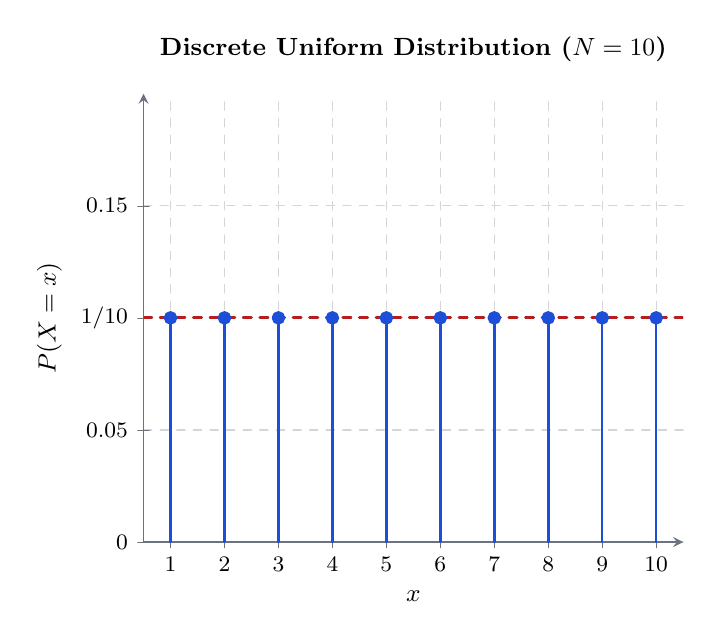
\begin{tikzpicture}
        \begin{axis}[
            title={Discrete Uniform Distribution ($N=10$)},
            xlabel={$x$},
            ylabel={$P(X=x)$},
            xmin=0.5, xmax=10.5,
            ymin=0, ymax=0.2,
            xtick={1,2,3,4,5,6,7,8,9,10},
            ytick={0, 0.05, 0.1, 0.15},
            yticklabels={0, 0.05, 1/10, 0.15},
            grid=major,
            grid style={dashed, gray!30},
            ymajorgrids=true,
            axis lines=left,
            enlarge x limits=false
        ]
            
            % Plot the stems (lollipops)
            \addplot[
                color=blue,
                thick,
                mark=*,
                ycomb,
            ] coordinates {
                (1, 0.1) (2, 0.1) (3, 0.1) (4, 0.1) (5, 0.1)
                (6, 0.1) (7, 0.1) (8, 0.1) (9, 0.1) (10, 0.1)
            };
            
            % Optional: Add a dashed line at 1/N to guide the eye
            \addplot[dashed, red, domain=0.5:10.5] {0.1};
            
        \end{axis}
    \end{tikzpicture}
    \caption{PMF of a Discrete Uniform Distribution where $P(X=x) = \frac{1}{10}$ for all $x$.}
\end{figure}













\begin{remark}
To derive the mean and variance, we utilize the standard power sum formulas: \[\sum_{i=1}^N i = \frac{N(N+1)}{2}\quad \text{and} \quad\sum_{i=1}^N i^2 = \frac{N(N+1)(2N+1)}{6}.\]
\end{remark}





\begin{thm} Moments of the distribution
\begin{enumerate} 
\item Mean (Expectation): \begin{align*} E(X) &= \sum_{x=1}^N x \cdot P(X=x)\\ 
&= \sum_{x=1}^N x \cdot \frac{1}{N} \\ 
&= \frac{1}{N} \sum_{x=1}^N x\\
& = \frac{1}{N} \left[ \frac{N(N+1)}{2} \right]\\ 
&= \frac{N+1}{2}. 
\end{align*}

\item Variance:
First, we calculate the second raw moment $E(X^2)$:
\begin{align*}
E(X^2) &= \sum_{x=1}^N x^2 \cdot \frac{1}{N}\\
       & = \frac{1}{N} \left[ \frac{N(N+1)(2N+1)}{6} \right] \\
       &= \frac{(N+1)(2N+1)}{6}.
\end{align*}
Using the identity $\operatorname{Var}(X) = E(X^2) - [E(X)]^2$:
\begin{align*}
\operatorname{Var}(X) &= \frac{(N+1)(2N+1)}{6} - \left( \frac{N+1}{2} \right)^2 \\
              &= \frac{N+1}{2} \left[ \frac{2N+1}{3} - \frac{N+1}{2} \right] \\
              &= \frac{N+1}{2} \left[ \frac{4N+2 - 3N - 3}{6} \right] \\
              &= \frac{(N+1)(N-1)}{12}\\
              & = \frac{N^2-1}{12}.
\end{align*}
\end{enumerate}
\end{thm}



\begin{thm} The transform functions for the Discrete Uniform distribution are based on the sum of a geometric progression.\begin{enumerate}
\item Probability Generating Function (PGF): For $t \neq 1$:$$ G_X(t) = E[t^X] = \sum_{x=1}^N t^x \frac{1}{N} = \frac{t(1-t^N)}{N(1-t)}. $$
\item Moment Generating Function (MGF):
For $t \neq 0$:
\[ M_X(t) = E[e^{tX}] = \sum_{x=1}^N e^{tx} \frac{1}{N} = \frac{e^t(1-e^{Nt})}{N(1-e^t)}. \]

\item Characteristic Function:
\[ \phi_X(t) = E[e^{itX}] = \frac{e^{it}(1-e^{iNt})}{N(1-e^{it})}. \]
\end{enumerate}
\end{thm}





\begin{remark}
To derive the mean $E(X)$ using the PGF, it is mathematically more convenient to differentiate the series expansion $\sum \frac{1}{N}t^x$ rather than the closed-form quotient. If the quotient form is used, one must apply L'Hôpital's Rule twice (for the second derivative) to resolve the indeterminate forms at $t=1$.
\end{remark}

\begin{proof}
\begin{enumerate}
\item Instead of using the ``shortcut'' formula, it is often easier to differentiate the summation form directly. This avoids the denominator issue entirely:$$ G_X'(t) = \frac{d}{dt} \left[ \sum_{x=1}^N \frac{1}{N}t^x \right] = \sum_{x=1}^N \frac{x}{N}t^{x-1} $$When we evaluate at $t=1$:$$ E(X) = G_X'(1) = \sum_{x=1}^N \frac{x}{N}(1)^{x-1} = \frac{1}{N} \sum_{x=1}^N x = \frac{N+1}{2} $$
\item The L'Hôpital's Rule Method (Using the Closed Form)If you insist on using the closed-form $G_X(t) = \frac{t(1-t^N)}{N(1-t)}$, you must use limits. 
\end{enumerate}
\end{proof}








\subsection{The Binomial Distribution}
The Binomial distribution models the number of successes in a sequence of $n$ independent trials, each with the same probability of success $p$. It is essentially the sum of $n$ independent and identically distributed (i.i.d.) Bernoulli random variables.

\begin{definition}
A random variable $X$ follows a Binomial distribution, denoted $X \sim \operatorname{Bin}(n, p)$, if its probability mass function (PMF) is:$$ f(x; n, p) = P(X=x) = \binom{n}{x} p^x (1-p)^{n-x}, \quad x = 0, 1, 2, \dots, n $$where $n$ is the number of trials and $p$ is the probability of success.
\end{definition}



\begin{remark}
If $X_1, X_2, \dots, X_n$ are i.i.d. Bernoulli random variables with parameter $p$, then the random variable $X = \sum_{i=1}^n X_i$ follows a Binomial distribution with parameters $n$ and $p$.
\end{remark}



\begin{figure}[H]
    \centering
    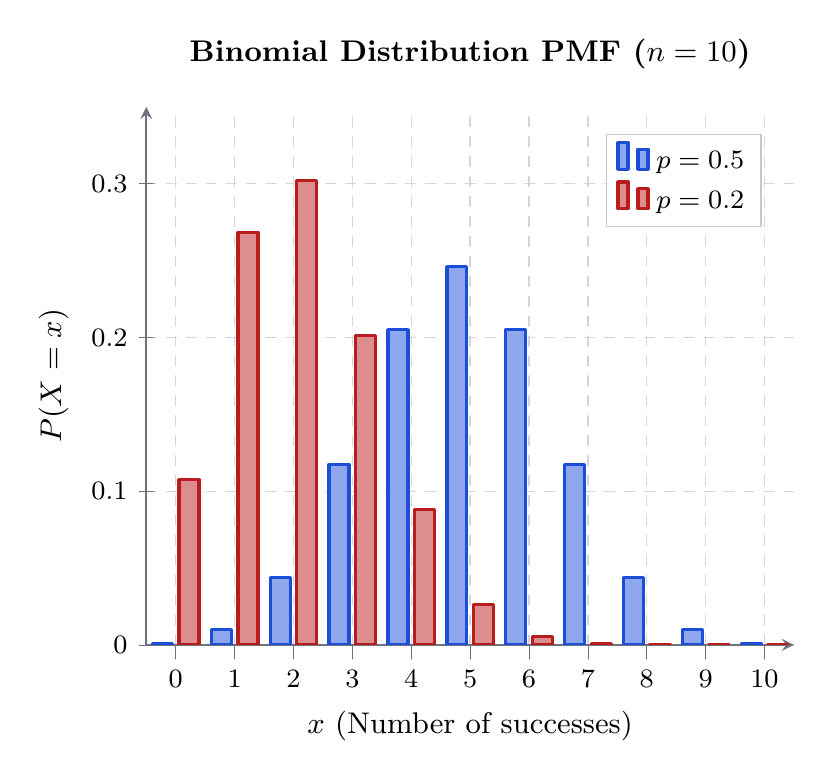
\begin{tikzpicture}[scale=1.2]
        \begin{axis}[
            title={Binomial Distribution PMF ($n=10$)},
            xlabel={$x$ (Number of successes)},
            ylabel={$P(X=x)$},
            xmin=-0.5, xmax=10.5,
            ymin=0, ymax=0.35,
            xtick={0,1,2,3,4,5,6,7,8,9,10},
            grid=major,
            grid style={dashed, gray!30},
            legend style={at={(0.95,0.95)}, anchor=north east},
            axis lines=left,
            ybar,
            bar width=6pt,
        ]
            
            % Case 1: p = 0.5 (Symmetric)
            \addplot[fill=blue!50, draw=blue] coordinates {
                (0, 0.0009) (1, 0.0098) (2, 0.0439) (3, 0.1172) (4, 0.2051) 
                (5, 0.2461) (6, 0.2051) (7, 0.1172) (8, 0.0439) (9, 0.0098) (10, 0.0009)
            };
            \addlegendentry{$p = 0.5$}

            % Case 2: p = 0.2 (Right-skewed)
            \addplot[fill=red!50, draw=red] coordinates {
                (0, 0.1074) (1, 0.2684) (2, 0.3020) (3, 0.2013) (4, 0.0881) 
                (5, 0.0264) (6, 0.0055) (7, 0.0008) (8, 0.0001) (9, 0.0000) (10, 0.0000)
            };
            \addlegendentry{$p = 0.2$}

        \end{axis}
    \end{tikzpicture}
    \caption{PMF of the Binomial distribution for $n=10$. Note the symmetry when $p=0.5$ and the right skew when $p=0.2$.}
\end{figure}



\begin{example}
A textile firm finds that only $20\%$ of applicants are qualified. If 5 people are interviewed, find the probability that at least two are qualified.
\end{example}
\begin{proof}[\textbf{Solution}]
Here $n=5$ and $p=0.2$ (so $q=0.8$). We want $P(X \ge 2)$:
\begin{align*}P(X \ge 2) &= 1 - P(X < 2)\\ 
& = 1 - [P(X=0) + P(X=1)]\\
&= 1 - \left[ \binom{5}{0}(0.2)^0(0.8)^5 + \binom{5}{1}(0.2)^1(0.8)^4 \right]\\
&= 1 - [0.32768 + 0.4096]\\
& = 0.26272.
\end{align*}
\end{proof}




\begin{remark}
Some identities
\begin{enumerate}
\item $x^{(k)}\binom{n}{x} = n^{(k)}\binom{n-k}{x-k}$
\item $x^{(k)} = x(x - 1)(x - 2) \cdots (x - k + 1)$
\item $\binom{x + k - 1}{x} = \binom{x + k - 1}{k - 1} = (-1)^x\binom{-k}{x}$
\end{enumerate}
\end{remark}






\begin{thm}
If $X \sim \operatorname{Bin}(n, p)$, the mean and variance are given by:
\begin{enumerate}
\item $E(X) = np$
\begin{proof}
Mean 
\begin{align*} 
E(X) &= \sum_{x=0}^n x \binom{n}{x} p^x (1-p)^{n-x}\\
& = \sum_{x=1}^n \frac{x \cdot n!}{x!(n-x)!} p^x (1-p)^{n-x}\\ 
& = np \sum_{x=1}^n \frac{(n-1)!}{(x-1)!(n-x)!} p^{x-1} (1-p)^{n-x}\\ 
& = np \sum_{y=0}^{n-1} \binom{n-1}{y} p^y (1-p)^{n-1-y} \quad (\text{letting } y = x-1)\\ 
& = np(p + (1-p))^{n-1}\\
& = np(1)^{n-1}\\
& = np. 
\end{align*}
\end{proof}


\item $\operatorname{Var}(X) = np(1-p)$
\begin{proof}
To find $\operatorname{Var}(X)$, we first find $E[X(X-1)]$:
\begin{align*}
E[X(X-1)] &= \sum_{x=2}^n x(x-1) \binom{n}{x} p^x (1-p)^{n-x}\\
&= \sum_{x=2}^n x^{(2)} \binom{n}{x} p^x (1-p)^{n-x}\\
&= n(n-1)p^2 \sum_{x=2}^n \binom{n-2}{x-2} p^{x-2} (1-p)^{n-x}\\
& = n(n-1)p^2.
\end{align*}
Since $E(X^2) = E[X(X-1)] + E(X) = n(n-1)p^2 + np$:
\begin{align*}
\operatorname{Var}(X) &= n(n-1)p^2 + np - (np)^2\\
& = n^2p^2 - np^2 + np - n^2p^2\\
& = np(1-p).
\end{align*}
\end{proof}
\end{enumerate}
\end{thm}


\begin{thm}
The generating functions for $X \sim \operatorname{Bin}(n, p)$ are:
\begin{enumerate}
\item Probability Generating Function (PGF):
\begin{align*}
G_X(t) &= E[t^X]\\
& = \sum_{x=0}^n t^x \binom{n}{x} p^x (1-p)^{n-x}\\
&= \sum_{x=0}^n \binom{n}{x} (pt)^x (1-p)^{n-x}\\
& = (pt + 1 - p)^n.
\end{align*}

\item Moment Generating Function (MGF):
\begin{align*}
M_X(t) &= E\left[e^{tx}\right]\\
& =\sum^n_{x=0}e^{tx}P(X=x)\\
&=\sum^n_{x=0}e^{tx}\binom{n}{x}p^x(1-p)^{n-x}\\
&=\sum^n_{x=0}\binom{n}{x}\left[pe^t\right]^x(1-p)^{n-x}\\
& = (pe^t+1-p)^n.
\end{align*}





\item Characteristic Function (CF):
$$ \phi_X(t) = E[e^{itX}] = (pe^{it} + 1 - p)^n. $$
\end{enumerate}\end{thm}




\subsection{The Hypergeometric Distribution}
\vspace{-15pt}
Consider a population of $N$ items, where $k$ items possess a certain characteristic (successes) and $N-k$ do not (failures). If a sample of $n$ items is drawn at random without replacement, let $X$ represent the number of successes in the sample.

\begin{definition}
A random variable $X$ follows a Hypergeometric distribution, denoted $X \sim \operatorname{Hyp}(N, n, k)$, if its probability mass function (PMF) is: $$ P(X=x) = \frac{\binom{k}{x}\binom{N-k}{n-x}}{\binom{N}{n}}, \quad x = \max(0, n-(N-k)), \dots, \min(n, k)$$
\end{definition}
\begin{figure}[H]
    \centering
    \begin{tikzpicture}[scale=0.7]
        \begin{axis}[
         %   title={Hypergeometric vs. Binomial Approximation},
            xlabel={$x$ (Number of successes)},
            ylabel={$P(X=x)$},
            xmin=-0.5, xmax=15.5,
            ymin=0, ymax=0.25,
            xtick={0,2,4,6,8,10,12,14},
            grid=major,
            grid style={dashed, gray!30},
            legend style={at={(0.95,0.95)}, anchor=north},
            axis lines=left,
            samples at={0,1,...,15},
        ]
            
            % Hypergeometric: N=100, k=30, n=20
            \addplot[
                only marks,
                mark=*,
                blue,
                thick
            ] {hypergeom(x, 100, 30, 20)};
            \addlegendentry{Hypergeometric ($N=100, k=30, n=20$)}

            % Binomial: n=20, p=k/N=0.3
            \addplot[
                red,
                sharp plot,
                dashed,
                thick
            ] {binom(20,x) * (0.3^x) * (0.7^(20-x))};
            \addlegendentry{Binomial ($n=20, p=0.3$)}

        \end{axis}
    \end{tikzpicture}
    \caption{The Hypergeometric distribution (dots) compared to the Binomial distribution (dashed line). As $N \to \infty$, these two distributions become identical.}
\end{figure}


\begin{example}
A shipment contains 100 items, of which $k$ are defective. A sample of size $n=2$ is selected. The shipment is accepted only if both items are non-defective ($X=0$).
\end{example}

\begin{proof}[\textbf{Solution}]The PMF for $N=100, n=2$ is $$P(X=x) = \frac{\binom{k}{x}\binom{100-k}{2-x}}{\binom{100}{2}}.$$\begin{enumerate}
\item[(i)] If $10\%$ are defective ($k=10$):$$ P(X=0) = \frac{\binom{10}{0}\binom{90}{2}}{\binom{100}{2}} = \frac{1 \cdot 4005}{4950} \approx 0.8091. $$
\item[(ii)] If $20\%$ are defective ($k=20$):$$ P(X=0) = \frac{\binom{20}{0}\binom{80}{2}}{\binom{100}{2}} = \frac{1 \cdot 3160}{4950} \approx 0.6384. $$
\end{enumerate}
\end{proof}








\begin{remark}
Vandermonde's Identity and Useful Relations:
\begin{equation}
\sum_{x = 0}^n \binom{k}{x}\binom{N-k}{n-x} = \binom{N}{n}\quad (\text{Ensures}\quad \sum P(X=x) = 1)
\end{equation}
\begin{equation}
x\binom{k}{x} = k\binom{k-1}{x - 1}
\end{equation}
\begin{equation}
n\binom{N}{n} = N\binom{N-1}{n-1}
\end{equation}
\end{remark}






\begin{lem}
If $X \sim \operatorname{Hyp}(N, n, k)$, then:
\begin{align*}
E\left[X^r\right] & = \sum^n_{x = 0}x^rP(X = x)\\
& = \sum^n_{x =1}\frac{x^r\, \binom{k}{x}\binom{N-k}{k-x}}{\binom{N}{n}}\\
& = n\sum^n_{x = 1}\frac{x^{r-1}\, k\binom{k-1}{x - 1}\binom{N-k}{n-x}}{N\binom{N-1}{n-1}}\quad (\text{by equ 2.4 and 2.5})\\
& = \frac{nk}{N}\sum^n_{x = 1}\frac{x^{r-1}\binom{k - 1}{x - 1}\binom{N - k}{n - x}}{\binom{N-1}{n-1}}\\
& = \frac{nk}{N}\sum^{n-1}_{y =0}\frac{(y + 1)^{r-1}\,\binom{k-1}{y}\binom{N-k}{n-1 - y}}{\binom{N-1}{n-1}}\\
& = \frac{nk}{N}\, E\left[(Y + 1)^{r-1}\right]
\end{align*}
where $Y \sim \operatorname{Hyp}(N-1, n-1, k-1)$
\end{lem}




\begin{thm}
If $X \sim \operatorname{Hyp}(N, n, k)$, then:$$ E(X) = \frac{nk}{N} \quad \text{and} \quad \operatorname{Var}(X) = \frac{nk}{N}\left(\frac{N-k}{N}\right)\left(\frac{N-n}{N-1}\right) $$
\end{thm}


\begin{proof}
Using the $r$-th moment relation derived: $E[X^r] = \frac{nk}{N} E[(Y+1)^{r-1}]$, where $Y \sim \operatorname{Hyp}(N-1, n-1, k-1)$.
\begin{enumerate}
\item \textbf{Mean ($r=1$):} $$E[X] = \frac{nk}{N} E[1] = \frac{nk}{N}.$$
\item \textbf{Variance:} First find $E[X(X-1)]$. By similar logic to the mean:$$ E[X(X-1)] = \frac{nk}{N} \cdot \frac{(n-1)(k-1)}{N-1}. $$Then, $\operatorname{Var}(X) = E[X(X-1)] + E(X) - [E(X)]^2$:
\begin{align*}
\operatorname{Var}(X) &= \frac{nk(n-1)(k-1)}{N(N-1)} + \frac{nk}{N} - \left(\frac{nk}{N}\right)^2\\
&= \frac{nk}{N} \left[ \frac{(n-1)(k-1)}{N-1} + 1 - \frac{nk}{N} \right]\\
&= \frac{nk(N-k)(N-n)}{N^2(N-1)}.
\end{align*}
\end{enumerate}
\end{proof}




\begin{remark}
\textbf{The Finite Population Correction:} The variance of the Hypergeometric distribution is the same as the Binomial variance ($npq$, where $q = \frac{N-k}{N}$), multiplied by the factor $\frac{N-n}{N-1}$. As $N \to \infty$, this factor approaches $1$, and the Hypergeometric converges to the Binomial.
\end{remark}




\begin{remark}
The hypergeometric has no closed form of MGF. $$\sum^{\min(n,k)}_{x=0}e^{tx}\frac{\binom{k}{x}\binom{N-k}{n-x}}{\binom{N}{n}}.$$
\end{remark}









\subsection{The Geometric Distribution}
The Geometric distribution models the number of independent Bernoulli trials required to achieve the first success. Unlike the Binomial distribution, which has a fixed number of trials $n$, the Geometric distribution has a fixed number of successes (one) and a variable number of trials.

\begin{definition}
A random variable $X$ follows a Geometric distribution, denoted $X \sim \operatorname{Geo}(p)$, if its probability mass function (PMF) is given by:$$ f(x; p) = P(X=x) = q^{x-1}p, \quad x = 1, 2, 3, \dots $$where $p$ is the probability of success and $q = 1-p$ is the probability of failure.
\end{definition}




\begin{figure}[H]
    \centering
    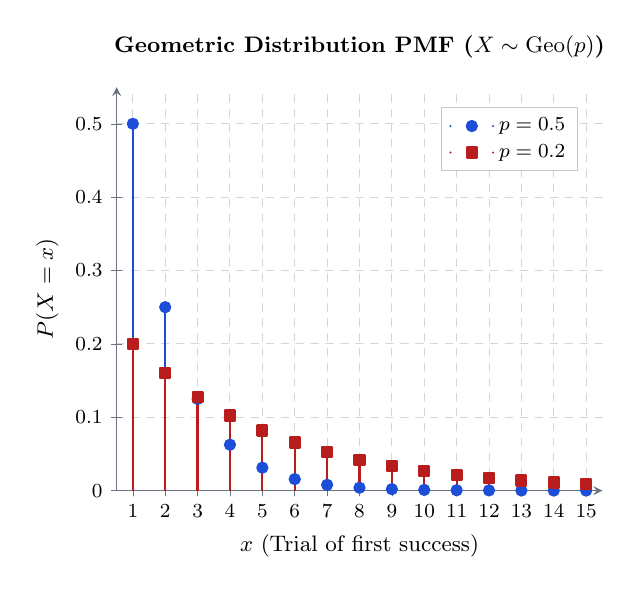
\begin{tikzpicture}[scale=0.9]
        \begin{axis}[
            title={Geometric Distribution PMF ($X \sim \operatorname{Geo}(p)$)},
            xlabel={$x$ (Trial of first success)},
            ylabel={$P(X=x)$},
            xmin=0.5, xmax=15.5,
            ymin=0, ymax=0.55,
            xtick={1,2,3,4,5,6,7,8,9,10,11,12,13,14,15},
            grid=major,
            grid style={dashed, gray!30},
            legend style={at={(0.95,0.95)}, anchor=north east},
            axis lines=left,
            samples at={1,2,...,15},
        ]
            
            % Case 1: p = 0.5 (Fast decay)
            \addplot[
                color=blue,
                mark=*,
                thick,
                ycomb,
            ] {0.5 * (0.5)^(x-1)};
            \addlegendentry{$p = 0.5$}

            % Case 2: p = 0.2 (Slow decay)
            \addplot[
                color=red,
                mark=square*,
                thick,
                ycomb,
            ] {0.2 * (0.8)^(x-1)};
            \addlegendentry{$p = 0.2$}

        \end{axis}
    \end{tikzpicture}
    \caption{PMF of the Geometric distribution. The probability decreases as the number of trials increases, illustrating that the first success is most likely to occur early.}
\end{figure}

















\subsubsection{Useful Results: Geometric Series}
To derive the moments of this distribution, we rely on the properties of the geometric series for $|t| < 1$:
\begin{enumerate}
\item $\sum_{x = 0}^{\infty} t^x = \frac{1}{1-t}$
\item $\sum_{x = 1}^{\infty} x t^{x-1} = \frac{d}{dt} \left( \sum_{x = 0}^{\infty} t^x \right) = \frac{1}{(1-t)^2}$
\item $\sum_{x = 2}^{\infty} x(x-1) t^{x-2} = \frac{d^2}{dt^2} \left( \sum_{x = 0}^{\infty} t^x \right) = \frac{2}{(1-t)^3}$
\end{enumerate}




\begin{example}
Show that the Geometric distribution in indeed a PMF
\end{example}
\begin{proof}
\begin{align*}
\sum^{\infty}_{x=1}P(X=x) &=\sum^{\infty}_{x=1}p(1-p)^{x-1}\\
                          &=p\sum^{\infty}_{x=1}(1-p)^{x-1}\\
                          &=p\sum^{\infty}_{k=0}(1-p)^k\,\quad\quad (\text{letting}\quad k = x - 1)\\
                          &=p\, \frac{1}{1-(1-p)}=\frac{p}{p}\\
                          &=1
\end{align*}
\end{proof}




\begin{thm}[\textbf{Moments of the Geometric Distribution}]
If $X \sim \operatorname{Geo}(p)$, then:
\begin{enumerate}
\item Mean: $$E(X) = \frac{1}{p}$$
\item Variance: $$\operatorname{Var}(X) = \frac{1-p}{p^2}$$
\end{enumerate}
\end{thm}


\begin{proof}
\textbf{1. Mean:} Using the second series result above:$$ E(X) = \sum_{x=1}^{\infty} x \cdot p q^{x-1} = p \sum_{x=1}^{\infty} x q^{x-1} = p \left( \frac{1}{(1-q)^2} \right) = p \left( \frac{1}{p^2} \right) = \frac{1}{p}. $$
\textbf{2. Variance:} First, we find the second factorial moment using the third series result:
\begin{align*}
E[X(X-1)] & = \sum_{x=1}^{\infty} x(x-1) p q^{x-1}\\
&  = pq \sum_{x=2}^{\infty} x(x-1) q^{x-2}\\
& = pq \left( \frac{2}{(1-q)^3} \right)\\
& = \frac{2pq}{p^3}\\
& = \frac{2q}{p^2}.
\end{align*} Using the identity $\operatorname{Var}(X) = E[X(X-1)] + E(X) - [E(X)]^2$:$$ \operatorname{Var}(X) = \frac{2q}{p^2} + \frac{1}{p} - \frac{1}{p^2} = \frac{2q + p - 1}{p^2} = \frac{2(1-p) + p - 1}{p^2} = \frac{1-p}{p^2}. $$
\end{proof}




\begin{thm} Transform Functions:
\begin{enumerate}
\item Probability Generating Function (PGF): $$ G_X(t) = E[t^X] = \sum_{x=1}^{\infty} t^x p q^{x-1} = pt \sum_{x=1}^{\infty} (qt)^{x-1} = \frac{pt}{1-qt}, \quad |t| < \frac{1}{q}. $$
\item Moment Generating Function (MGF):$$ M_X(t) = E[e^{tX}] = \frac{pe^t}{1-qe^t}, \quad t < -\ln(q). $$
\end{enumerate}
\end{thm}



\begin{thm}[\textbf{Memoryless Property}]
The Geometric distribution is the only discrete distribution with the memoryless property:$$ P(X > i+j \mid X > i) = P(X > j) $$This means that the probability of needing $j$ more trials to get a success does not depend on how many failed trials ($i$) have already occurred.
\end{thm}









\begin{example}
In a large production batch, $5\%$ of items are defective. A quality control inspector tests items one by one until the first defective item is found.
\begin{enumerate}
\item[(i)] Find the probability that the first defective item is the $10^{th}$ item tested.
\item[(ii)] Find the expected number of items the inspector must test.
\end{enumerate}
\end{example}

\begin{proof}[\textbf{Solution}]
Let $X$ be the number of items tested until the first defective. Here, $p = 0.05$ and $q = 0.95$.
\begin{enumerate}
\item[(i)] $P(X=10) = q^{10-1}p = (0.95)^9(0.05) \approx 0.0315$.
\item[(ii)] $E(X) = \frac{1}{p} = \frac{1}{0.05} = 20$ items.
\end{enumerate}
\end{proof}


















\subsection{The Negative Binomial Distribution}
The Negative Binomial distribution models the number of independent Bernoulli trials required to achieve a fixed number of successes, denoted by $r$. It is often referred to as the Pascal distribution or the waiting time distribution.


\begin{definition}
A random variable $X$ follows a Negative Binomial distribution, denoted $X \sim \operatorname{NB}(r, p)$, if its probability mass function (PMF) is:$$ f_X(x) = \binom{x-1}{r-1} p^r (1-p)^{x-r}, \quad x = r, r+1, r+2, \dots $$where $p$ is the probability of success in each trial.
\end{definition}




\begin{figure}[H]
    \centering
    \begin{tikzpicture}[scale=0.9]
        \begin{axis}[
            title={Negative Binomial PMF ($p=0.4$)},
            xlabel={$x$ (Total trials)},
            ylabel={$P(X=x)$},
            xmin=0, xmax=25,
            ymin=0, ymax=0.2,
            grid=major,
            grid style={dashed, gray!30},
            legend style={at={(0.95,0.95)}, anchor=north east},
            axis lines=left,
        ]
            % r = 2
            \addplot[blue, mark=*, thick, samples at={2,3,...,25}] {nbinom(x, 2, 0.4)};
            \addlegendentry{$r=2$}

            % r = 5
            \addplot[red, mark=square*, thick, samples at={5,6,...,25}] {nbinom(x, 5, 0.4)};
            \addlegendentry{$r=5$}
        \end{axis}
    \end{tikzpicture}
    \caption{Negative Binomial Distribution for $r=2$ and $r=5$. Note how the distribution starts at $x=r$.}
\end{figure}












\subsubsection{The Two Versions of the Distribution} In probability theory, there are two common ways to define this random variable:
\begin{enumerate}
\item \textbf{Number of trials ($X$):} The total number of trials required to get $r$ successes ($x \in \{r, r+1, \dots\}$).
\item \textbf{Number of failures ($Y$):} The number of failures encountered before the $r^{th}$ success occurs ($y \in \{0, 1, \dots\}$).
\end{enumerate}
The relationship is simply $Y = X - r$. The PMF for the number of failures $Y$ is:$$ f_Y(y) = \binom{y+r-1}{r-1} p^r (1-p)^y, \quad y = 0, 1, 2, \dots $$




\begin{thm}
If $X \sim \operatorname{NB}(r, p)$, then:
\begin{enumerate}
\item Mean: $$E(X) = \frac{r}{p}$$
\item Variance: $$\operatorname{Var}(X) = \frac{r(1-p)}{p^2}$$
\end{enumerate}
\end{thm}

\begin{proof} Recall that $X$ can be viewed as the sum of $r$ independent Geometric random variables, $X = X_1 + X_2 + \dots + X_r$, where each $X_i \sim \operatorname{Geo}(p)$.Using the linearity of expectation:$$ E(X) = E\left(\sum_{i=1}^r X_i\right) = \sum_{i=1}^r E(X_i) = \sum_{i=1}^r \frac{1}{p} = \frac{r}{p}. $$Since the trials are independent:$$ \operatorname{Var}(X) = \operatorname{Var}\left(\sum_{i=1}^r X_i\right) = \sum_{i=1}^r \operatorname{Var}(X_i) = \sum_{i=1}^r \frac{1-p}{p^2} = \frac{r(1-p)}{p^2}. $$
\end{proof}

\begin{thm}[\textbf{Generating Functions}]
For the version $Y$ (number of failures):
\begin{enumerate}
\item Probability Generating Function (PGF): $$G_Y(t) = \left( \frac{p}{1-qt} \right)^r$$
\item Moment Generating Function (MGF): $$M_Y(t) = \left( \frac{p}{1-qe^t} \right)^r, \quad t < -\ln(q)$$
\end{enumerate}
\end{thm}




\begin{example}A scientist inoculates mice one at a time until 3 contract a disease. If the probability of contracting the disease is $1/6$, what is the probability that exactly 8 mice are required?
\end{example}
\begin{proof}[\textbf{Solution}] Here $r=3$ (target successes) and $p=1/6$ (success probability). We want the probability that the $3^{rd}$ success occurs on the $8^{th}$ trial ($x=8$).$$ P(X=8) = \binom{8-1}{3-1} \left(\frac{1}{6}\right)^3 \left(\frac{5}{6}\right)^{8-3} = \binom{7}{2} \left(\frac{1}{216}\right) \left(\frac{3125}{7776}\right) $$$$ P(X=8) = 21 \cdot \frac{3125}{1679616} \approx 0.0391. $$
\end{proof}















\subsection{The Poisson Distribution}
The Poisson distribution is a discrete probability distribution that models the number of independent events occurring within a fixed interval of time or space. It is uniquely characterized by a single parameter, $\lambda$ (lambda), which represents the constant average rate of occurrence.

Typical applications include:\begin{itemize}
\item The number of calls received by a telecommunications switchboard per minute.
\item The number of radioactive particles decayed from a source within a second.
\item The number of typographical errors found in a single page of a manuscript.
\end{itemize}



\begin{definition}
A discrete random variable $X$ is said to follow a \textit{Poisson distribution} with parameter $\lambda > 0$, denoted as $X \sim \text{Po}(\lambda)$, if its probability mass function (PMF) is:$$ f(x; \lambda) = P(X=x) = \frac{e^{-\lambda} \lambda^x}{x\!}, \quad x = 0, 1, 2, \dots $$
\end{definition}



% Insert the diagram of the Poisson
\begin{figure}[H]
    \centering
    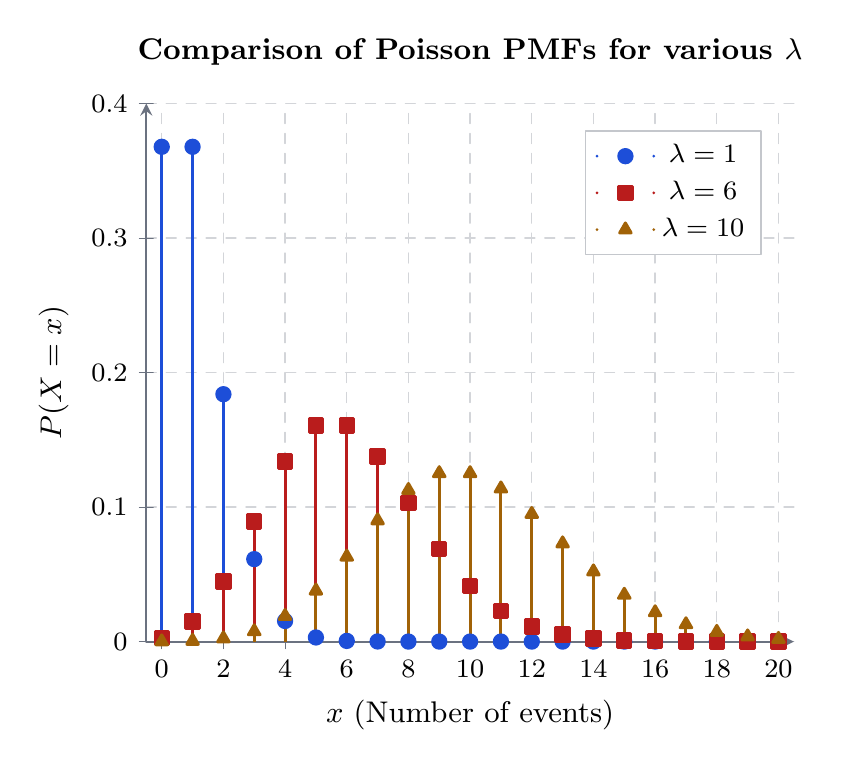
\begin{tikzpicture}[scale=1.2]
        \begin{axis}[
            title={Comparison of Poisson PMFs for various $\lambda$},
            xlabel={$x$ (Number of events)},
            ylabel={$P(X=x)$},
            xmin=-0.5, xmax=20.5,
            ymin=0, ymax=0.4,
            xtick={0,2,4,6,8,10,12,14,16,18,20},
            grid=major,
            grid style={dashed, gray!30},
            legend style={at={(0.95,0.95)}, anchor=north east},
            axis lines=left,
            samples at={0,1,...,20}, % This defines the discrete points
        ]
            
            % Lambda = 1
            \addplot[
                color=blue,
                mark=*,
                thick,
                ycomb,
            ] {exp(-1) * (1^x) / (factorial(x))};
            \addlegendentry{$\lambda = 1$}

            % Lambda = 4
            \addplot[
                color=red,
                mark=square*,
                thick,
                ycomb,
            ] {exp(-6) * (6^x) / (factorial(x))};
            \addlegendentry{$\lambda = 6$}

            % Lambda = 10
            \addplot[
                color=orange,
                mark=triangle*,
                thick,
                ycomb,
            ] {exp(-10) * (10^x) / (factorial(x))};
            \addlegendentry{$\lambda = 10$}
            
        \end{axis}
    \end{tikzpicture}
    \caption{Probability Mass Function of the Poisson Distribution showing the effect of the rate parameter $\lambda$.}
\end{figure}



\begin{example}
Verify that $f(x; \lambda)$ is a valid probability mass function.
\end{example}
\begin{proof}
A valid PMF must satisfy $\sum_{x} f(x) = 1$. Using the Taylor series expansion for the exponential function $e^\lambda = \sum_{x=0}^{\infty} \frac{\lambda^x}{x!}$:
\begin{align*}
\sum_{x = 0}^{\infty} f_X(x) &= \sum^{\infty}_{x = 0}\frac{e^{-\lambda} \lambda^x}{x!}\\
&= e^{-\lambda} \sum^{\infty}_{x = 0} \frac{\lambda^x}{x!}\\
& = e^{-\lambda} e^{\lambda} = 1.
\end{align*}
\end{proof}


     







\begin{thm}
If $X\thicksim \operatorname{PO}(\lambda)$, then 
\begin{enumerate}
\item mean is $\, E(X) = \lambda$.
\begin{proof}
Using the definition of expectations
\begin{align*}
E(X) & = \sum_{x = 0}^{\infty}x, \frac{e^{-\lambda}\, \lambda^x}{x!}\\
& = e^{-\lambda}\sum^{\infty}_{x = 1}\frac{x\,\lambda^x}{x(x-1)!} \\
& = \lambda e^{-\lambda}\sum^{\infty}_{x = 1} \frac{\lambda^{x - 1}}{(x - 1)!}\\
& = \lambda e^{-\lambda}\, \sum^{\infty}_{y = 0} \frac{\lambda^y}{y!}\, ,\quad\quad \text{letting}\quad y = x - 1\\
& = \lambda e^{-\lambda}\, e^{\lambda}\\
& = \lambda.
\end{align*}
\end{proof}


\item variance is $\, \operatorname{Var}(X) = \lambda$.
\begin{proof}
We first compute $E(X^2)$:
\begin{align*}
E(X^2) & = \sum^{\infty}_{x = 0} \frac{x^2\, e^{-\lambda}\, \lambda^x}{x!}\\
& = \lambda\, e^{-\lambda} \sum^{\infty}_{x = 1}\frac{x\cdot x\, \lambda^{x - 1}}{x(x-1)!} \\
& = \lambda\, e^{-\lambda}\sum^{\infty}_{x = 1} \frac{x\, \lambda^{x - 1}}{(x - 1)!}\\
& = \lambda \, e^{-\lambda} \sum_{y = 0}^{\infty}\frac{(y+1)\, \lambda^{y}}{y!}\, , \quad\quad \text{letting}\quad y = x - 1\\
& = \lambda\left[\sum^{\infty}_{y = 0}\frac{y\,e^{-\lambda}\, \lambda^y}{y!} + \sum^{\infty}_{y = 0}\frac{e^{-\lambda}\, \lambda^y}{y!}\right]\\
& = \lambda(\lambda + 1).
\end{align*}
Therefore, the variance
\begin{align*}
\operatorname{Var}(X) & = E(X^2) - \left[E(X)\right]^2\\
& = \lambda^2 + \lambda - [\lambda]^2\\
& = \lambda.
\end{align*}
\end{proof}
\end{enumerate}
\end{thm}

 


\begin{thm}
If $X\thicksim \operatorname{POI}(\lambda)$, then 
\begin{enumerate}
\item Probability Generating Function (PGF):
\begin{align*}
G_X(t) = E[t^X] & = \sum_{x=0}^{\infty} t^x\,\, \frac{e^{-\lambda} \lambda^x}{x!}\\
& = e^{-\lambda} \sum_{x=0}^{\infty} \frac{(\lambda t)^x}{x!}\\
& = e^{-\lambda} e^{\lambda t}\\
& = e^{\lambda(t-1)}. 
\end{align*}


\item Moment Generating Function (MGF):
\begin{align*}
M_X(t) = E[e^{tX}] & = \sum_{x=0}^{\infty} e^{tx} \frac{e^{-\lambda} \lambda^x}{x!}\\
&  = e^{-\lambda} \sum_{x=0}^{\infty} \frac{(\lambda e^t)^x}{x!}\\
& = e^{-\lambda} e^{\lambda e^t}\\
& = e^{\lambda(e^t-1)}.
\end{align*}

\item Characteristic Function:
\[ \phi_X(t) = E[e^{itX}] = e^{\lambda(e^{it}-1)}. \]
\end{enumerate}
\end{thm}




\begin{remark}[{\textbf{The Poisson Process}}] A Poisson experiment satisfies the following properties: 
\begin{enumerate} 
\item[(i)] \textbf{Independence:} The number of outcomes in one time interval is independent of the number in any other disjoint interval. 
\item[(ii)] \textbf{Proportionality:} The probability of a single outcome occurring in a very short interval is proportional to the length of the interval. 
\item[(iii)] \textbf{Negligibility:} The probability of more than one outcome occurring in a sufficiently short interval is negligible. 
\end{enumerate} 
\end{remark}

\begin{example} The average number of calls coming into a switchboard is 4 per minute. Assuming a Poisson distribution, find the probability that: 
\begin{enumerate} 
\item[(i)] Exactly 5 calls are received. 
\item[(ii)] More than one call is received. 
\end{enumerate} 
\end{example}


\begin{proof}[\textbf{Solution}]
Here, $\lambda = 4$.
\begin{enumerate}
\item[(i)] $P(X=5) = \frac{4^5 e^{-4}}{5!} \approx 0.1563$.
\item[(ii)] $P(X > 1) = 1 - P(X \leq 1) = 1 - [P(0) + P(1)]$.
\begin{align*}
P(X > 1) &= 1 - \left[ \frac{4^0 e^{-4}}{0!} + \frac{4^1 e^{-4}}{1!} \right]\\
&= 1 - [e^{-4} + 4e^{-4}]\\
& = 1 - 5e^{-4} \\
& \approx 1 - 0.09158 = 0.9084.
\end{align*}
\end{enumerate}
\end{proof}







\begin{thm}[\textbf{Poisson Approximation to the Binomial}]
If $n$ is large ($n \to \infty$) and $p$ is small ($p \to 0$), the Binomial distribution $\operatorname{B}(n, p)$ can be approximated by a Poisson distribution with $\lambda = np$.
\end{thm}




\begin{example}
Suppose that on average one person in every 1, 000 has an eye problem. Find the probability that a random sample of 8, 000 people will have fever than 7 people with eye problem.
\end{example}


\begin{proof}[\textbf{\textit{Solution}}]
Given 
\begin{enumerate}
\item[ ] $X = $ number with eye problem
\item[ ] $p = $ probabilities of having an eye problem
\item[ ] $p = 0.001$
\item[ ] $n = $ number of independent trials
\item[ ] $n = 8000$
\end{enumerate}
\[P(X=x) = \binom{n}{x} p^x(1-p)^{n-x}\]
\[
P(X<7) = \sum^6_{x=0}\binom{8000}{x}(0.001)^x(0.999)^{8000-x}.\]
Which is tedious to complete. We use Poisson approximation to Binomial
\[\lambda = np =8000\times 0.001 = 8.\]
\begin{align*}
P(X<7) & = P(X\leq 6)\\
& = \sum^6_{x=0}\frac{8^xe^{-8}}{x!}\\
&= e^{-8}\left(\frac{8^0}{0!}+\frac{8}{1!}+\frac{8^2}{2!}+\frac{8^3}{3!}+\frac{8^4}{4!}+\frac{8^5}{5!}+\frac{8^6}{6!}\right)\\
&=0.3134
\end{align*}
\end{proof}












\subsection{The Zeta (or Zipf) Distribution}
\vspace{-10pt}
The Zeta distribution, frequently referred to as the Zipf distribution, is a power-law distribution typically utilized to model the frequency of occurrences of data in diverse fields such as linguistics, economics, and social sciences. It effectively accounts for ``long-tail'' phenomena where a small number of members in a population account for a high proportion of the total frequency (popularity), while the majority remain in relative obscurity. Notable applications include the distribution of family incomes, the frequency of words in a language, and the population sizes of cities.


\begin{definition}
A discrete random variable $X$ is said to have a Zeta distribution with parameter $\alpha$, denoted $X \sim \operatorname{Zeta}(\alpha)$, if its probability mass function is given by:$$f(x; \alpha) = \frac{x^{-\alpha}}{\zeta(\alpha)}, \quad x = 1, 2, 3, \dots$$for $\alpha > 1$, where $\zeta(\alpha)$ is the \textbf{Riemann Zeta Function} defined by the infinite series:$$\zeta(\alpha) = \sum_{n=1}^{\infty}\,\frac{1}{n^{\alpha}}.$$
\end{definition}


\begin{note}
Observe that the support of $X$ starts at $x=1$. If the summation in the denominator were to start at $x=0$, the term $0^{-\alpha}$ would be undefined for $\alpha > 1$.
\end{note}

% Insert Diagram of the Zeta
\begin{figure}[H]
    \centering
    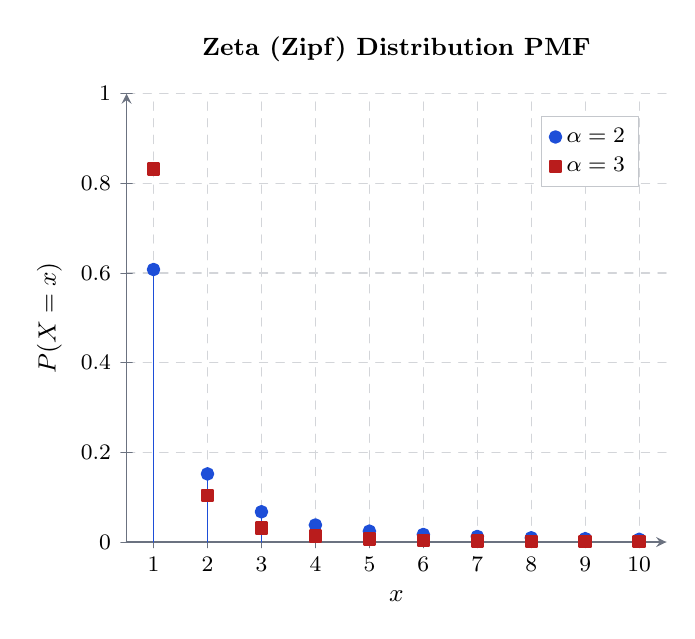
\begin{tikzpicture}
        \begin{axis}[
            title={Zeta (Zipf) Distribution PMF},
            xlabel={$x$},
            ylabel={$P(X=x)$},
            xmin=0.5, xmax=10.5,
            ymin=0, ymax=1,
            xtick={1,2,3,4,5,6,7,8,9,10},
            grid=major,
            grid style={dashed, gray!30},
            legend style={at={(0.95,0.95)}, anchor=north east}
        ]
            
            % Zeta PMF for alpha = 2
            % zeta(2) is approximately 1.645
            \addplot[
                color=blue,
                mark=*,
                thick,
                only marks
            ] coordinates {
                (1, 0.6079) (2, 0.1520) (3, 0.0675) (4, 0.0380) (5, 0.0243)
                (6, 0.0169) (7, 0.0124) (8, 0.0095) (9, 0.0075) (10, 0.0061)
            };
            \addlegendentry{$\alpha = 2$}

            % Zeta PMF for alpha = 3
            % zeta(3) is approximately 1.202
            \addplot[
                color=red,
                mark=square*,
                thick,
                only marks
            ] coordinates {
                (1, 0.8319) (2, 0.1040) (3, 0.0308) (4, 0.0130) (5, 0.0067)
                (6, 0.0039) (7, 0.0024) (8, 0.0016) (9, 0.0011) (10, 0.0008)
            };
            \addlegendentry{$\alpha = 3$}
            
            % Stems for alpha = 2
            \addplot[ycomb, blue, no marks, thin] coordinates {
                (1, 0.6079) (2, 0.1520) (3, 0.0675) (4, 0.0380) (5, 0.0243)
                (6, 0.0169) (7, 0.0124) (8, 0.0095) (9, 0.0075) (10, 0.0061)
            };

        \end{axis}
    \end{tikzpicture}
    \caption{Probability Mass Function of the Zeta Distribution for $\alpha=2$ and $\alpha=3$.}
\end{figure}




\begin{thm}If $X \sim \operatorname{Zeta}(\alpha)$, the moments of the distribution are defined as follows:
\begin{enumerate}
\item Mean $$E(X) = \frac{\zeta(\alpha - 1)}{\zeta(\alpha)},$$ provided $\alpha > 2$.
\begin{proof}By the definition of expectation
\begin{align*}
E(X) &= \sum_{x=1}^{\infty} x \cdot f(x; \alpha)\\
& = \frac{1}{\zeta(\alpha)} \sum_{x=1}^{\infty} x \cdot \frac{1}{x^{\alpha}}\\ 
&= \frac{1}{\zeta(\alpha)} \sum_{x=1}^{\infty} \frac{1}{x^{\alpha - 1}}\\
& = \frac{\zeta(\alpha - 1)}{\zeta(\alpha)}.
\end{align*}For the series $\zeta(\alpha - 1)$ to converge, we require $\alpha - 1 > 1$, thus $\alpha > 2$.
\end{proof}
\item Variance $$\operatorname{Var}(X) = \frac{\zeta(\alpha)\zeta(\alpha-2) - \zeta(\alpha-1)^2}{\zeta(\alpha)^2},$$ provided $\alpha > 3$.
\begin{proof}
First, we determine the second raw moment:
\[ E(X^2) = \sum_{x=1}^{\infty} x^2 \frac{1}{x^{\alpha} \zeta(\alpha)} = \frac{1}{\zeta(\alpha)} \sum_{x=1}^{\infty} \frac{1}{x^{\alpha - 2}} = \frac{\zeta(\alpha - 2)}{\zeta(\alpha)}. \]
Applying the variance formula $\operatorname{Var}(X) = E(X^2) - [E(X)]^2$:
\begin{align*}
\operatorname{Var}(X) &= \frac{\zeta(\alpha - 2)}{\zeta(\alpha)} - \left( \frac{\zeta(\alpha - 1)}{\zeta(\alpha)} \right)^2 \\
&= \frac{\zeta(\alpha)\zeta(\alpha - 2) - \zeta(\alpha - 1)^2}{\zeta(\alpha)^2}.
\end{align*}
The term $\zeta(\alpha - 2)$ converges only if $\alpha - 2 > 1$, hence $\alpha > 3$.
\end{proof}
\end{enumerate}
\end{thm}



\begin{thm}
The transform functions for $X \sim \operatorname{Zeta}(\alpha)$ are characterized by the following series:
\begin{enumerate}
\item Probability Generating Function: $$G_X(t) = E\left[t^X\right] = \frac{1}{\zeta(\alpha)} \sum_{x=1}^{\infty} \frac{t^x}{x^{\alpha}}, \quad\quad |t| \le 1.$$
\item Moment Generating Function: $$M_X(t) = E\left[e^{tX}\right] =  \frac{1}{\zeta(\alpha)} \sum_{x=1}^{\infty} \frac{e^{tx}}{x^{\alpha}}, \quad\quad  t \le 0.$$
\item Characteristic Function: $$\phi_X(t) = E\left[e^{itX}\right] =  \frac{1}{\zeta(\alpha)} \sum_{x=1}^{\infty} \frac{e^{itx}}{x^{\alpha}}.$$
\end{enumerate}
\end{thm}
%%%%%%%%%%%%%%%%%%%%%%%%%%%%%%%%%%%%%%%%%%%%%%%%%%%%%%%%%%%%%%%%%%%%%%%%%%%%%%%%%%%%%%%%%%%%%%%%%%%%%%%%%%%%%%%%%%%%
















\section{Some Important Continuous Probability Density Functions}
\vspace{-15pt}
In this section, we describe models frequently used in continuous random phenomena. These distributions are the building blocks of statistical inference and engineering applications.


\subsection{The Uniform Distribution}
\vspace{-15pt}
The uniform distribution provides a probability model for selecting points at random from an $[\alpha , \beta]$. An important application of the uniform distribution lies in random number generation. 


\begin{definition}[\textbf{Uniform Distribution $X \thicksim \operatorname{UNIF}(\alpha, \beta)$}]
A random variable $X$ is said to be uniform on the interval $[\alpha, \beta]$ if its p.d.f. is of the form
\[ f_X(x)=
\begin{cases}
\dfrac{1}{\beta -\alpha}, & \quad \alpha \leq x\leq \beta\\
0, &\text{otherwise}\\
\end{cases}
\]
\end{definition}



\subsubsection{Diagrams of the Uniform Distribution.}
\begin{figure}[H]
\centering
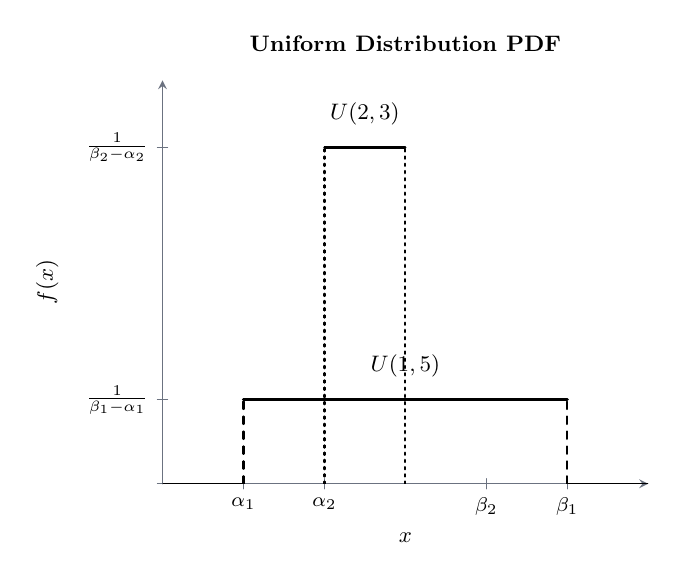
\begin{tikzpicture}[scale=0.9]
\begin{axis}[
    axis lines = left,
    xlabel = $x$,
    ylabel = {$f(x)$},
    xmin = 0, xmax = 6,
    ymin = 0, ymax = 1.2,
    xtick = {1, 2, 4, 5},
    xticklabels = {$\alpha_1$, $\alpha_2$, $\beta_2$, $\beta_1$},
    ytick = {0.25, 1},
    yticklabels = {$\frac{1}{\beta_1-\alpha_1}$, $\frac{1}{\beta_2-\alpha_2}$},
    title = {Uniform Distribution PDF},
    extra y ticks={0},
    extra y tick labels={}
]

% Case 1: Wide interval [1, 5], Height = 1/4 = 0.25
% We draw the vertical dashed lines to show the boundaries
\draw [black, thick, dashed] (axis cs: 1, 0) -- (axis cs: 1, 0.25);
\draw [black, thick, dashed] (axis cs: 5, 0) -- (axis cs: 5, 0.25);
\addplot [black, ultra thick] coordinates {(1, 0.25) (5, 0.25)};
\node at (axis cs: 3, 0.35) {\small $U(1, 5)$};

% Case 2: Narrow interval [2, 4], Height = 1/2 = 0.5 (Adjusted for visual clarity)
% Note: Using [2, 3] Height = 1 for a more dramatic comparison
\draw [black, thick, dotted] (axis cs: 2, 0) -- (axis cs: 2, 1);
\draw [black, thick, dotted] (axis cs: 3, 0) -- (axis cs: 3, 1);
\addplot [black, thick] coordinates {(2, 1) (3, 1)};
\node at (axis cs: 2.5, 1.1) {\small $U(2, 3)$};

% Drawing the baseline on the x-axis for "otherwise = 0"
\addplot [black, thin] coordinates {(0,0) (1,0)};
\addplot [black, thin] coordinates {(5,0) (6,0)};

\end{axis}
\end{tikzpicture}
\caption{The PDF of the Uniform distribution. Note that the total area under each rectangle is exactly $1$.}
\end{figure}




The mean of $X$ is
\begin{align*}
E(X) &=\int^{\beta}_{\alpha}x\frac{1}{\beta -\alpha}\, dx\\
&=\frac{1}{\beta -\alpha}\int^{\beta}_{\alpha}x\, dx\\
&=\frac{\alpha^2}{2(\beta -\alpha)}\Bigg|_{\alpha}^{\beta}\\
&=\frac{\beta^2-\alpha^2}{2(\beta -\alpha)}\\
&=\frac{(\beta +\alpha)(\beta-\alpha)}{2(\beta-\alpha)}\\
& =\frac{\beta +\alpha}{2}.
\end{align*}
Also
\begin{align*}
E(X^2) & = \frac{1}{\beta - \alpha}\int^{\beta}_{\alpha} x^2\,dx\\
& = \frac{1}{\beta - \alpha}\left[\frac{x^3}{3}\right]^{\beta}_{\alpha}\\
& = \frac{1}{\beta-\alpha}\, \frac{\beta^3-\alpha^3}{3}\\
& = \frac{(\beta - \alpha)(\beta^2 + \beta \alpha + \alpha^2)}{3(\beta - \alpha)}\\
& = \frac{\beta^2 + \beta \alpha + \alpha^2}{3}.
\end{align*}
Hence, variance is
\begin{align*}
\operatorname{Var}(X) & = \frac{\beta^2 + \beta \alpha + \alpha^2}{3}- \frac{(\beta + \alpha)^2}{4}\\
& = \frac{\beta^2 - 2\beta \alpha + \alpha^2}{12}\\
& = \frac{(\beta - \alpha)^2}{12}.
\end{align*}

The m.g.f of $X$ is 
\begin{align*}
M_X(t) &=E\left(e^{tx}\right)\\
&=\int^{\beta}_{\alpha}e^{tx}\, dx\\ 
&=\frac{1}{\beta -\alpha}\int^{\beta}_{\alpha}e^{tx}\, dx\\
& =\frac{1}{\beta -\alpha}\,\frac{e^{tx}}{t}\Bigg|_{\alpha}^{\beta}\\
 &=\frac{e^{\beta t}-e^{\alpha t}}{t(\beta-\alpha)}.
\end{align*}
Thus \[M_X(t)= \begin{cases}
\frac{e^{\beta t}-e^{\alpha t}}{t(\beta-\alpha)}\, , & \text{if}\,\, t \neq 0\\
1, & \text{if}\,\, t = 0.\\
\end{cases}.\]

\begin{remark}
Foundation of Simulation: In computer science and computational statistics, the ``Random'' function in almost all programming languages generates a $U(0, 1)$ value. Other distributions (like Normal or Exponential) are then generated by transforming these uniform values using the Inverse Transform Method.
\end{remark}





\subsection{Exponential Distribution}
\vspace{-15pt}
The exponential is the distribution of the amount of time until some specific event occurs (i.e waiting time). For instance, how long one waits before a new component ``dies''?



\begin{definition}
A continuous random variable $X$ whose p.d.f is given, for some $\lambda > 0$, by 
\[ f_X(x)=
\begin{cases}
\lambda e^{-\lambda x}, & x >0,\quad \lambda>0\\
0, &\text{otherwise}\\
\end{cases}
\]
is said to be an exponential random variable.
\end{definition}



\begin{remark}
An exponential has the mean and variable 
\[E(X)=\frac{1}{\lambda},\quad \operatorname{Var}(X)=\frac{1}{\lambda^2}.\]
\end{remark}

\begin{note}
The p.d.f of an exponential random variable can also be presented in this form
\[ f_X(x)=
\begin{cases}
\frac{1}{\lambda}e^{-\frac{x}{\lambda}}, & x>0,\quad \lambda>0\\
0, &\text{otherwise}
\end{cases}
\]
where the mean and variance are
\[E(X)=\lambda, \quad \operatorname{Var}(X)=\lambda^2.\]
\end{note}



\subsubsection{Graphs of an Exponential}
\begin{figure}[H]
\centering
%--- Left Side: Rate Parameterization ---
\begin{minipage}{0.48\textwidth}
    \centering
    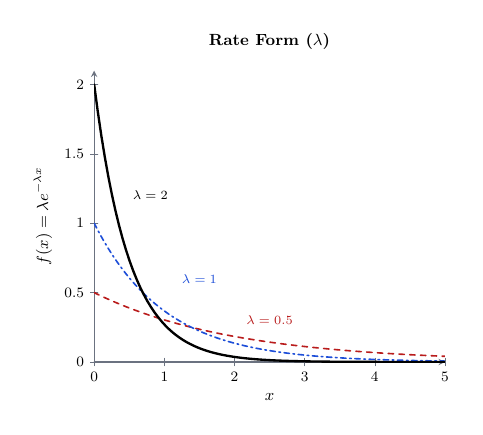
\begin{tikzpicture}[scale=0.65]
    \begin{axis}[
        axis lines = left,
        xlabel = $x$,
        ylabel = {$f(x) = \lambda e^{-\lambda x}$},
        domain = 0:5,
        samples = 100,
        ymin = 0, ymax = 2.1,
        title={Rate Form ($\lambda$)}
    ]
    % lambda = 0.5
    \addplot [red, thick, dashed] {0.5 * exp(-0.5*x)};
    \node[red] at (axis cs: 2.5, 0.3) {\scriptsize $\lambda=0.5$};
    
    % lambda = 1
    \addplot [blue, thick, dashdotted] {1 * exp(-1*x)};
    \node[blue] at (axis cs: 1.5, 0.6) {\scriptsize $\lambda=1$};
    
    % lambda = 2
    \addplot [ ultra thick, solid] {2 * exp(-2*x)};
    \node at (axis cs: 0.8, 1.2) {\scriptsize $\lambda=2$};
    \end{axis}
    \end{tikzpicture}
\end{minipage}
\hfill
%--- Right Side: Scale Parameterization ---
\begin{minipage}{0.48\textwidth}
    \centering
    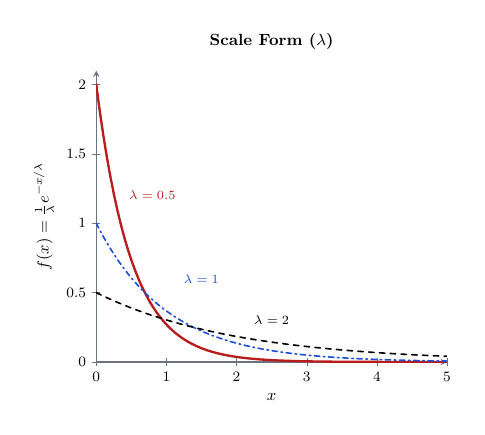
\begin{tikzpicture}[scale=0.65]
    \begin{axis}[
        axis lines = left,
        xlabel = $x$,
        ylabel = {$f(x) = \frac{1}{\lambda} e^{-x/\lambda}$},
        domain = 0:5,
        samples = 100,
        ymin = 0, ymax = 2.1,
        title={Scale Form ($\lambda$)}
    ]
    % lambda = 0.5 (Narrower, higher start)
    \addplot [red, ultra thick, solid] {(1/0.5) * exp(-x/0.5)};
    \node[red] at (axis cs: 0.8, 1.2) {\scriptsize $\lambda=0.5$};
    
    % lambda = 1
    \addplot [blue, thick, dashdotted] {(1/1) * exp(-x/1)};
    \node[blue] at (axis cs: 1.5, 0.6) {\scriptsize $\lambda=1$};
    
    % lambda = 2 (Flatter, lower start)
    \addplot [black, thick, dashed] {(1/2) * exp(-x/2)};
    \node at (axis cs: 2.5, 0.3) {\scriptsize $\lambda=2$};
    \end{axis}
    \end{tikzpicture}
\end{minipage}

\caption{Comparison of Exponential Distribution parameterizations. Note how increasing $\lambda$ makes the Rate Form (left) ``taller,'' but makes the Scale Form (right) ``flatter.''}
\end{figure}


\begin{note}[\textbf{Important}]
\textbf{ }
\begin{enumerate}
\item \textit{Rate Parameterization $(\lambda)$:} Used most commonly in Poisson processes. Here, $E(X) = \frac{1}{\lambda}$. As $\lambda$ increases, the mean decreases, and the curve becomes steep.
\item \textit{Scale Parameterization $(\theta$ or $\lambda)$:} Often used in engineering and reliability (Mean time to failure). Here, $E(X) = \lambda$. As $\lambda$ increases, the mean increases, the curve spreads out further along the $x$-axis. 
\end{enumerate}
\end{note}




The cumulative distribution function is
\begin{align*}
F_X(x) & = P[X \leq x]\\
& = \int^x_0 \lambda \, e^{-\lambda x}\, dx\\
& = -e^{-\lambda x}\Big|^x_0\\
& = 1 - e^{-\lambda x}\, , \quad x \geq 0.
\end{align*}


The moment generating function is 
\begin{align*}
M_X(t) & = E\left[e^{tX}\right]\\
& = \int^{\infty}_0 e^{tx}\, \lambda e^{-\lambda x}\, dx\\
& = \lambda \int^{\infty}_0 e^{-(\lambda - t)x}\, dx\\
& = \frac{\lambda}{\lambda - t}\,,  \quad t < \lambda.
\end{align*}

Then differentiating $M'_X(t)$ we get
\[M'_X(t) = \frac{\lambda (-1) (-1)}{(\lambda - t)^2} = \frac{\lambda}{(\lambda - t})^2\]
\[M''_X(t) = \frac{\lambda (-1)(-2)}{(\lambda - t)^3} = \frac{2\lambda}{(\lambda - t)^3}\]
Then the mean is 
\[E(X) = M'_X(0) = \frac{\lambda}{\lambda^2} = \frac{1}{\lambda}\]
and 
\[E(X^2) = M''_X(0) = \frac{2\lambda}{\lambda^3} = \frac{2}{\lambda^2}\]
then variance
\[\operatorname{Var}(X) = \frac{2}{\lambda^2}-\left(\frac{1}{\lambda^2}\right) = \frac{1}{\lambda^2}.\]






















\begin{example}
A manufacture of microwave ovens is trying to determine the length of warranty period it should attach to its magneto tube, the most critical component in the microwave oven. Preliminary testing has shown that the life of the tube has an exponential distribution with mean 6.25 years.
\begin{enumerate}
\item[(i).] What is the warranty period if the manufacturer wants to replace only $10\%$ of the magneto tube.
\begin{proof}[\textit{Solution}]
Let the warranty period be $\alpha$.
$X\thicksim $ Exp$(\lambda)$, $E(X)=6.25$
$$f_X(x)=\frac{1}{6.25}e^{-\frac{x}{6.25}}$$
$P(X\leq \alpha)=0.1$
\begin{align*}
\int^{\alpha}_0\frac{1}{6.25}e^{-\frac{x}{6.25}}dx=0.1\\
 -e^{-\frac{x}{6.25}}\Bigg|_0^{\alpha} &=0.1\\
1-e^{-\frac{\alpha}{6.25}}=0.1\\ e^{-\frac{\alpha}{6.25}} &=0.90\hspace{0.5cm} \implies\frac{-\alpha}{6.25}=\ln (0.90)\\ \alpha &=-6.25 \ln (0.90).
\end{align*}
Therefore, $\alpha =0.6585$\, years \, $\approx 7.9$ months $\approx 8.0$\,  months.
\end{proof}


\item[(ii).] If the warranty is 4 years, what percentage of the tubes will be replaced?
\begin{proof}[\textbf{\textit{Solution}}]
\begin{align*}
P(X\leq 4) &=\int^4_0\frac{1}{6.25}e^{-\frac{x}{6.25}}dx\\
& =-e^{-\frac{x}{6.25}}\Big|_0^4\\
& = 1-e^{-\frac{4}{6.25}}\\
& = 0.4727 = 47.27\%
\end{align*}
\end{proof}
\end{enumerate}
\end{example}







\subsection{Gamma Distribution}
\begin{definition}[\textbf{Gamma Function}]
The gamma function, denoted by $\Gamma(\alpha)$  for all $\alpha > 0$, is given by \[\Gamma(\alpha) = \int_0^{\infty} t^{\alpha - 1}\, e^{-t}\, dt.\]
\end{definition}


\subsubsection{Properties of $\Gamma$}
\begin{enumerate}
\item[(i).] $\Gamma (\alpha + 1) = \alpha\,\Gamma(\alpha)$
\item[(ii).] $\Gamma(n) = (n-1)!, \, n = 1, 2, \cdots$
\item[(iii).] $\Gamma\left(\frac{1}{2}\right) = \sqrt{\pi}$
\end{enumerate}




\begin{definition}[\textbf{Gamma Distribution $X\thicksim \operatorname{GAM}(\alpha, \lambda)$}]
A gamma random variable $X$ with parameters $\alpha > 0, \, \lambda > 0$, has probability density function 
\[f_X(x) =\frac{x^{\alpha -1}e^{-\frac{x}{\lambda}}}{\lambda^{\alpha}\Gamma(\alpha)}\quad \text{or}\quad f_X(x) =\frac{\lambda^{\alpha}x^{\alpha-1}e^{-\lambda x}}{\Gamma(\alpha)}\, , \quad\quad  x>0\]
\end{definition}


\begin{note}
When $\alpha = 1$, then the gamma reduces to the exponential distribution.
\[f_X(x)  = \frac{x^{1-1}e^{-\frac{x}{\lambda}}}{\lambda^1 \Gamma(1)}=\frac{1}{\lambda}e^{-\frac{x}{\lambda}},\quad x>0,\quad\lambda >0\]
\[f_X(x)  = \frac{\lambda^1x^{1-1}e^{-\lambda x}}{\Gamma(1)}=\lambda e^{-\lambda x},\quad x>0,\quad \lambda >0\]
\end{note}




The moment generating function of $X$ is
\begin{align*}
M_X(t) &=E\left[e^{tx}\right]
=\int^{\infty}_{0} e^{tx}\,\frac{\lambda^{\alpha}\, x^{\alpha - 1}\, e^{-\alpha\lambda}}{\Gamma(\alpha)}\, dx\\
& = \frac{\alpha^{\lambda}}{\Gamma(\alpha)}\int^{\infty}_0x^{\alpha - 1}\, e^{-(\lambda - t)x}\, dx\\
& =\frac{\lambda^{\alpha}}{\Gamma(\alpha)}\int^{\infty}_0\left(\frac{y}{\lambda -t}\right)^{\alpha -1}e^{-y}\, \frac{dy}{\lambda -t},\quad\quad\quad \text{letting}\quad y = (\lambda - t)x\\
&=\frac{\lambda^{\alpha}}{\Gamma(\alpha)}\frac{1}{(\lambda -t)^{\alpha-1}}\,\frac{1}{(\lambda - t)}\int^{\infty}_{0}y^{\alpha-1}\, e^{-y}\, dy\\ 
&=\frac{\lambda^{\alpha}}{\Gamma(\alpha)}\quad\left(\frac{1}{\lambda -t}\right)^{\alpha}\quad\Gamma(\alpha)\\
&=\left(\frac{\lambda}{\lambda-t}\right)^{\alpha}.
\end{align*}

Differentiating $M_X(t)$
\begin{align*}
M'_X(t) &  = \lambda^{\alpha}(-\alpha)(\lambda -t)^{-\alpha -1}(-1) = \alpha \lambda^{\alpha}(\lambda -t)^{-\alpha-1} = \frac{\alpha\, \lambda^{\alpha}}{(\lambda - t)^{\alpha + 1}}\\ 
M''_X(t) & = \frac{\alpha \, [-(\alpha + 1)](-1)\,\lambda^{\alpha}}{(\lambda - t)^{\alpha + 2}}=\frac{\alpha (\alpha + 1) \lambda^{\alpha}}{(\lambda - t)^{\alpha + 2}}
\end{align*}
Then the mean is 
\[E(X) = M'_X(0) = \frac{\alpha\, \lambda^{\alpha}}{\lambda^{\alpha + 1}}= \frac{\alpha}{\lambda}\]
and  for the  variance  
\[E(X^2) = M''_X(0) = \frac{\alpha(\alpha + 1) \, \lambda^{\alpha}}{\lambda^{\alpha + 2}} = \frac{\alpha (\alpha + 1)}{\lambda^{2}}\]
therefore
\[\operatorname{Var}(X) = \frac{\alpha^2 + \alpha}{\lambda^2} - \left(\frac{\alpha}{\lambda}\right)= \frac{\alpha}{\lambda^2}.\]






\begin{remark}
\textbf{ }
\begin{enumerate}
\item We can present the m.g.f of the gamma as \[M_X(t)=\left(\frac{\lambda}{\lambda -t}\right)^{\alpha}=\left(\frac{1}{1-t/\lambda}\right)^{\alpha}=\left(1-\frac{t}{\lambda}\right)^{-\alpha}.\]
\item The ``Shape'' parameter ($\alpha$) dictates the physical appearance of the curve (as seen in plots below), while the ``Rate'' parameter ($\lambda$) determines the scale or ``spread'' of the data along the $x$-axis.
\item While the Exponential distribution models the time until the first event occurs in a Poisson process, the Gamma distribution models the time required for $\alpha$ independent events to occur.
\item The gamma is a sum of independent exponentials. Exponential is  $X\thicksim \operatorname{GAM}(1,\lambda).$
\end{enumerate}
\end{remark}


\begin{example}
The lifetime of a battery is exponentially distributed with rate $\lambda$. If a stereo cassette requires one battery to operate, then the total playing time one can obtain from the total of $n$ batteries is a gamma random variable with parameters $(n,\lambda)$.
\end{example}




\subsubsection{Graphs of the Gamma}
%\begin{figure}[H]
%\centering
%\begin{tikzpicture}
%\begin{axis}[
%    axis lines = left,
%    xlabel = $x$,
%    ylabel = {$f(x; \alpha, \lambda)$},
%    domain = 0:7,
%    samples = 150,
%    ymin = 0, ymax = 1.2,
%    xmin = 0,
%    restrict y to domain=0:1.5,
%    legend pos = north east,
%    legend style={draw=none, fill=none, font=\small},
%    title={Gamma PDF for various $\alpha$ ($\lambda=1$)}
%]

%% alpha = 0.5 (Decaying curve, starts at infinity)
%\addplot [cyan, thick, dotted] {1 * x^(-0.5) * exp(-x) / 1.772};
%\addlegendentry{$\alpha = 0.5$}
%\node at (axis cs: 0.4, 1.1) [anchor=west] {\scriptsize $\alpha=0.5$};

%% alpha = 1 (The Exponential case from your equation)
%\addplot [black, ultra thick, solid] {exp(-x)};
%\addlegendentry{$\alpha = 1$}
%\node at (axis cs: 1.2, 0.4) [anchor=south west] {\scriptsize $\alpha=1$};

%% alpha = 2
%\addplot [orange, thick, dashed] {x * exp(-x)};
%\addlegendentry{$\alpha = 2$}
%\node at (axis cs: 2.2, 0.38) [anchor=south] {\scriptsize $\alpha=2$};

%% alpha = 3
%\addplot [red, thick, dashdotted] {0.5 * x^2 * exp(-x)};
%\addlegendentry{$\alpha = 3$}
%\node at (axis cs: 3.5, 0.28) [anchor=south] {\scriptsize $\alpha=3$};

%% alpha = 4
%\addplot [blue, line width=1pt, loosely dashed] {(1/6) * x^3 * exp(-x)};
%\addlegendentry{$\alpha = 4$}
%\node at (axis cs: 4.8, 0.2) [anchor=south] {\scriptsize $\alpha=4$};

%\end{axis}
%\end{tikzpicture}
%\caption{Comparison of Gamma distributions for different values of $\alpha$.}
%\end{figure}


\begin{figure}[H]
\centering
%--- Left Side: Varying Alpha ---
\begin{minipage}{0.48\textwidth}
    \centering
    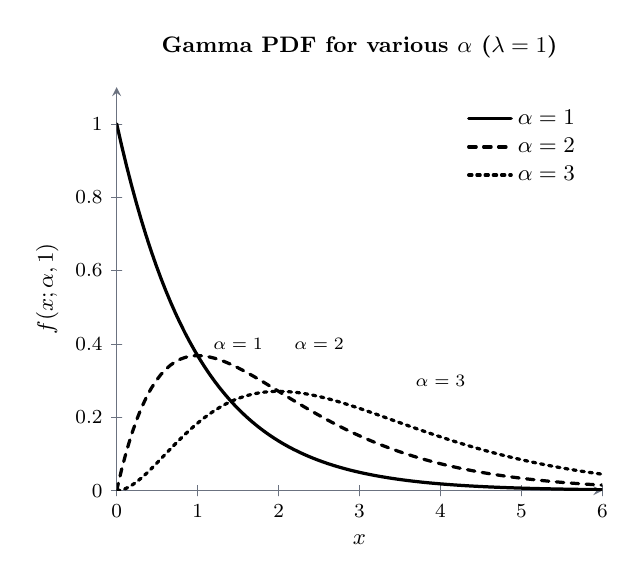
\begin{tikzpicture}[scale=0.9]
    \begin{axis}[
        axis lines = left,
        xlabel = $x$,
        ylabel = {$f(x;\alpha,1)$},
        domain = 0:6,
        samples = 100,
        ymin = 0, ymax = 1.1,
        legend pos = north east,
        legend style={draw=none, fill=none, font=\small},
        title={Gamma PDF for various $\alpha$ ($\lambda =1$)},
        %subtitle={fixed $\lambda=1$}
    ]
    % alpha = 1
    \addplot [black, ultra thick] {exp(-x)};
    \addlegendentry{$\alpha = 1$}
    \node at (axis cs: 1.5, 0.4) {\scriptsize $\alpha=1$};
    
    % alpha = 2
    \addplot [black, ultra thick, dashed] {x * exp(-x)};
    \addlegendentry{$\alpha = 2$}
    \node at (axis cs: 2.5, 0.4) {\scriptsize $\alpha=2$};
    
    % alpha = 3
    \addplot [black, ultra thick, dotted] {0.5 * x^2 * exp(-x)};
    \addlegendentry{$\alpha = 3$}
    \node at (axis cs: 4, 0.3) {\scriptsize $\alpha=3$};
    \end{axis}
    \end{tikzpicture}
\end{minipage}
\hfill
%--- Right Side: Varying Lambda ---
\begin{minipage}{0.48\textwidth}
    \centering
    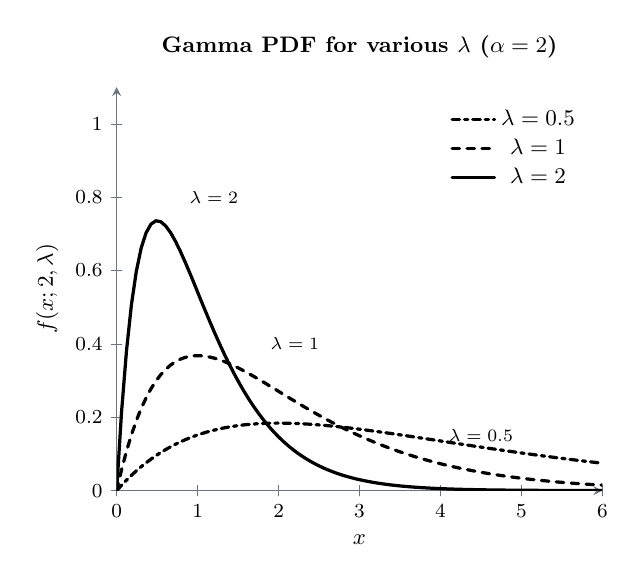
\begin{tikzpicture}[scale=0.9]
    \begin{axis}[
        axis lines = left,
        xlabel = $x$,
        ylabel = {$f(x;2,\lambda)$},
        domain = 0:6,
        samples = 100,
        ymin = 0, ymax = 1.1,
        legend pos = north east,
        legend style={draw=none, fill=none, font=\small},
        title={Gamma PDF for various $\lambda$ ($\alpha = 2$)},
        %subtitle={fixed $\alpha=2$}
    ]
    % lambda = 0.5 (Wider)
    \addplot [black, ultra thick, dashdotted] {0.5^2 * x * exp(-0.5*x)};
    \addlegendentry{$\lambda = 0.5$}
    \node at (axis cs: 4.5, 0.15) {\scriptsize $\lambda=0.5$};
    
    % lambda = 1 (Standard)
    \addplot [black, ultra thick, dashed] {1^2 * x * exp(-1*x)};
    \addlegendentry{$\lambda = 1$}
    \node at (axis cs: 2.2, 0.4) {\scriptsize $\lambda=1$};
    
    % lambda = 2 (Taller/Narrower)
    \addplot [black, ultra thick] {2^2 * x * exp(-2*x)};
    \addlegendentry{$\lambda = 2$}
    \node at (axis cs: 1.2, 0.8) {\scriptsize $\lambda=2$};
    \end{axis}
    \end{tikzpicture}
\end{minipage}

\caption{Comparison of Gamma distribution parameters. Left: Changing shape ($\alpha$) shifts the peak and changes the skew. Right: Changing rate ($\lambda$) affects the spread and height.}
\end{figure}





















\subsection{Beta Distribution}
\begin{definition}[\textbf{Beta Function.}]
We define the \textit{Beta} function of $\alpha$ and $\beta$, by \[B(\alpha,\beta) = \int^1_0t^{\alpha-1}\,(1 - t)^{\beta - 1}\, dt\] for $\alpha > 0$ and $\beta > 0$.
\end{definition}



\subsubsection{Properties of $B$:}
\begin{enumerate}
\item $B(\alpha, \beta) = \frac{\Gamma(\alpha)\, \Gamma(\beta)}{\Gamma(\alpha + \beta)}$
\item $B(\alpha, \beta) = B(\beta, \alpha)$
\item $B(\alpha + 1, \beta) = \frac{\alpha}{\alpha + \beta}\, B(\alpha, \beta)$
\item $B(\alpha , \beta + 1) = \frac{\beta}{\alpha + \beta}\, B(\alpha,\beta)$
\end{enumerate}

\begin{definition}[\textbf{Beta Distribution $X\thicksim \operatorname{Beta}(\alpha,\beta)$}]
A random variable is said to have a \textit{beta distribution} if its density p.d.f is given by 
\[f_X(x)=\frac{x^{\alpha -1}(1-x)^{\beta -1}}{B(\alpha,\beta)}\, , \quad\quad\alpha >0, \quad \beta >0, \quad 0<x<1.\]
\end{definition}



The $k^{\text{th}}$ expectation of  $X$ is
\begin{align*}
E(x^k) & = \int\limits_x x^kf_X(x)\,dx\\
& =\int^1_0\frac{x^k\, x^{\alpha-1}\, (1-x)^{\beta-1}}{B(\alpha,\beta)}\,dx\\
       & = \frac{1}{B(\alpha,\beta)}\int^1_0x^{k+\alpha-1}(1-x)^{\beta-1}\,dx\\
       & = \frac{1}{B(\alpha,\beta)}B(k+\alpha,\beta)\\
       & = \frac{\dfrac{\Gamma(k+\alpha)\Gamma(\beta)}{\Gamma(k+\alpha+\beta)}}{\dfrac{\Gamma(\alpha)\Gamma(\beta)}{\Gamma(\alpha+\beta)}}
        =\frac{\Gamma(k+\alpha)\Gamma(\beta)}{\Gamma(k+\alpha+\beta)}\times \frac{\Gamma(\alpha+\beta)}{\Gamma(\alpha)\Gamma(\beta)}\\
  & = \frac{\Gamma(k+\alpha)\Gamma(\alpha+\beta)}{\Gamma(\alpha)\Gamma(k+\alpha+\beta)}.
\end{align*}


When $k = 1$, we get the mean of $X$
\[E(x)=\frac{\Gamma(\alpha+1)\Gamma(\alpha+\beta)}{\Gamma(\alpha)\Gamma(\alpha+\beta+1)}=\frac{\alpha\Gamma(\alpha)\Gamma(\alpha+\beta)}{\Gamma(\alpha)(\alpha+\beta)\Gamma(\alpha+\beta)}=\frac{\alpha}{\alpha+\beta}.\]



When $k = 2$, we get 
\begin{align*}
E(x^2)  & = \frac{\Gamma(\alpha+2)\Gamma(\alpha+\beta)}{\Gamma(\alpha)\Gamma(\alpha+\beta+2)}\\
      &  = \frac{(\alpha+1)\alpha\Gamma(\alpha)\Gamma(\alpha+\beta)}{\Gamma(\alpha)(\alpha+\beta+1)(\alpha+\beta)\Gamma(\alpha+\beta)}\\
       & = \frac{\alpha(\alpha+1)}{(\alpha+\beta+1)(\alpha+\beta)}.
\end{align*}


Therefore, the variance of $X$ is
\begin{align*}
\operatorname{Var}(x) & = E(x^2)-(E(x))^2\\
 &=\frac{\alpha(\alpha+1)}{(\alpha+\beta)(\alpha+\beta+1)}-\left(\frac{\alpha}{\alpha+\beta}\right)^2\\
                                      & = \frac{\alpha}{\alpha+\beta}\left[\frac{\alpha+1}{\alpha+\beta+1}-\frac{\alpha}{\alpha+\beta}\right]\\
                                      & = \frac{\alpha}{\alpha+\beta}\left[\frac{(\alpha+1)(\alpha+\beta)-\alpha(\alpha+\beta+1)}{(\alpha+\beta)(\alpha+\beta+1)}\right]\\
                                      & = \frac{\alpha}{(\alpha+\beta)^2}\left[\frac{\alpha^2+\alpha\beta+\alpha+\beta-\alpha^2-\alpha\beta-\alpha}{\alpha+\beta+1}\right]\\
                                      & = \frac{\alpha\beta}{(\alpha+\beta)^2(\alpha+\beta+1)}.                                            
\end{align*}




\subsubsection{Graph of the Beta Distribution.}
\begin{figure}[H]
\centering
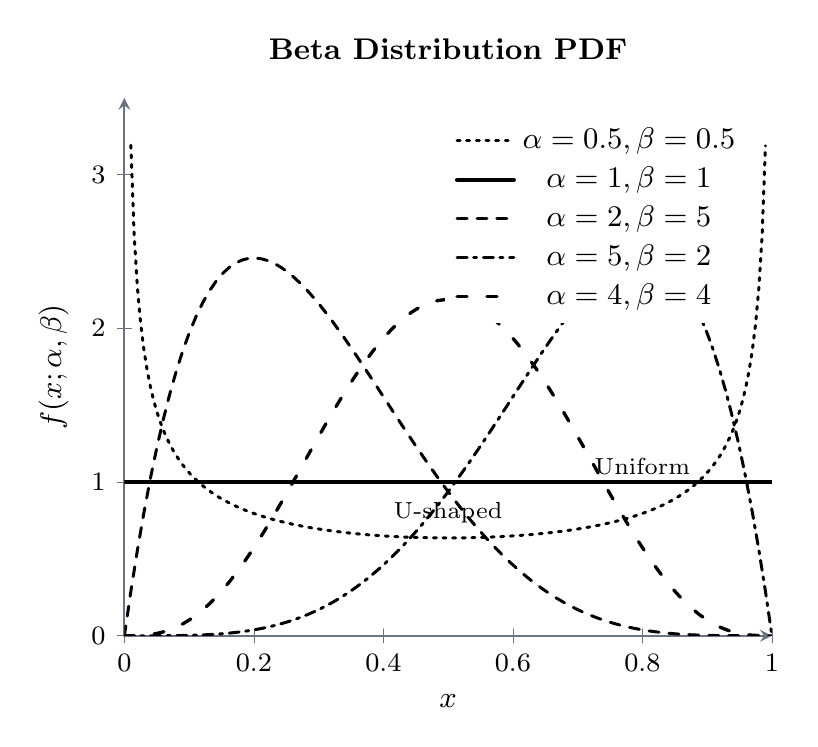
\begin{tikzpicture}[scale=1.2]
\begin{axis}[
    axis lines = left,
    xlabel = {$x$},
    ylabel = {$f(x; \alpha, \beta)$},
    domain = 0:1,
    samples = 100,
    ymin = 0, ymax = 3.5,
    xmin = 0, xmax = 1,
    legend pos = north east,
    legend style={draw=none, font=\small},
    title = {Beta Distribution PDF}
]

% Case 1: alpha=0.5, beta=0.5 (U-shaped)
\addplot [black, thick, dotted, samples=200, restrict y to domain=0:4] 
    { (x^(-0.5) * (1-x)^(-0.5)) / 3.1415 };
\addlegendentry{$\alpha=0.5, \beta=0.5$}
\node at (axis cs: 0.5, 0.8) {\scriptsize U-shaped};

% Case 2: alpha=1, beta=1 (Uniform Distribution)
\addplot [black, ultra thick, solid] {1};
\addlegendentry{$\alpha=1, \beta=1$}
\node at (axis cs: 0.8, 1.1) {\scriptsize Uniform};

% Case 3: alpha=2, beta=5 (Right-skewed)
% B(2,5) = 1/30
\addplot [black, thick, dashed] { 30 * x^(2-1) * (1-x)^(5-1) };
\addlegendentry{$\alpha=2, \beta=5$}

% Case 4: alpha=5, beta=2 (Left-skewed)
% B(5,2) = 1/30
\addplot [black, thick, dashdotted] { 30 * x^(5-1) * (1-x)^(2-1) };
\addlegendentry{$\alpha=5, \beta=2$}

% Case 5: alpha=4, beta=4 (Symmetric/Bell-shaped)
% B(4,4) = 1/140
\addplot [black, line width=1pt, loosely dashed] { 140 * x^(4-1) * (1-x)^(4-1) };
\addlegendentry{$\alpha=4, \beta=4$}

\end{axis}
\end{tikzpicture}
\caption{The Beta distribution takes various shapes depending on $\alpha$ and $\beta$, making it ideal for modeling proportions and probabilities.}
\end{figure}



\begin{remark}
The Beta distribution is famously known as the ``Probability of a Probability.'' In Bayesian statistics, it is used as the conjugate prior for the Bernoulli and Binomial distributions. For example, if you are trying to estimate the probability of success of a new crop variety in a specific Zambian province, the Beta distribution represents your ``certainty'' about that probability.
\end{remark}






\subsection{Normal Distribution}
\vspace{-15pt}
The main importance of normal distribution lies on the central limit theorem which says that the sample mean has a normal distribution if the sample size is large. 



\begin{definition}[\textbf{Normal Distribution $X\thicksim N(\mu,\sigma^2)$}]
A random variable $X$ is said to normally distributed, with parameter $\mu$ and $\sigma^2$ if the density of $X$ is given by
\[f_X(x)=\frac{1}{\sqrt{2\pi \sigma^2}}\, e^{-\frac{1}{2\sigma^2}(x-\mu)^2}\, ,\quad x\ \in (-\infty,\infty).\]
\end{definition}


This density function is a bell-shaped curve that is symmetric about $\mu$. However, the special normal distribution is the standard normal distribution denoted by 
\[Z\thicksim N(0,1)\implies \mu =0,\quad \sigma^2=1.\]



\begin{figure}[H]
\centering
%--- Left Side: Standard Normal ---
\begin{minipage}{0.48\textwidth}
    \centering
    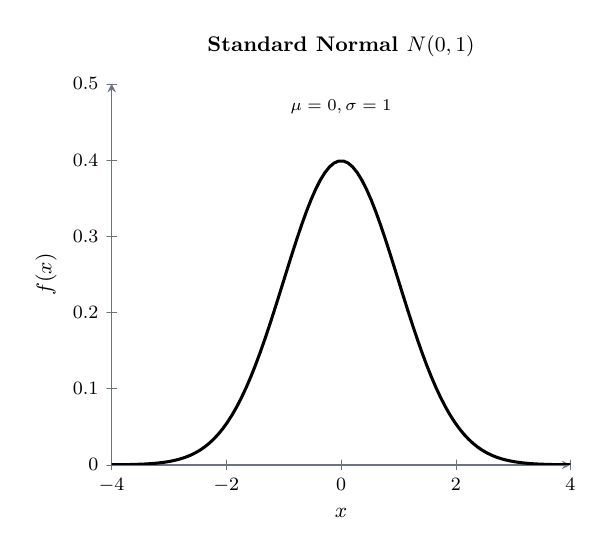
\begin{tikzpicture}[scale=0.85]
    \begin{axis}[
        axis lines = left,
        xlabel = $x$,
        ylabel = {$f(x)$},
        domain = -4:4,
        samples = 100,
        ymin = 0, ymax = 0.5,
        title={Standard Normal $N(0,1)$}
    ]
    % mu=0, sigma=1
    \addplot [black, ultra thick] {exp(-x^2/2)/sqrt(2*pi)};
    \node at (axis cs: 0, 0.45) [anchor=south] {\scriptsize $\mu=0, \sigma=1$};
    \end{axis}
    \end{tikzpicture}
\end{minipage}
\hfill
%--- Right Side: General Normal ---
\begin{minipage}{0.48\textwidth}
    \centering
    \begin{tikzpicture}[scale=0.85]
    \begin{axis}[
        axis lines = left,
        xlabel = $x$,
        ylabel = {$f(x)$},
        domain = -2:10,
        samples = 100,
        ymin = 0, ymax = 0.5,
        title={General Normal $N(\mu, \sigma^2)$}
    ]
    % mu=4, sigma=1.5
    % Formula: (1/(1.5 * sqrt(2*pi))) * exp(-0.5 * ((x-4)/1.5)^2)
    \addplot [black, thick, dashed] { (1/(1.5*sqrt(2*pi))) * exp(-0.5*((x-4)/1.5)^2) };
    \node at (axis cs: 4, 0.3) [anchor=south] {\scriptsize $\mu=4, \sigma=1.5$};
    \end{axis}
    \end{tikzpicture}
\end{minipage}

\caption{Comparison between the Standard Normal distribution and a General Normal distribution with shifted mean and increased variance.}
\end{figure}


\begin{thm}
If $X \thicksim N(\mu,\sigma^2)$, then
\begin{align*}
E(X) & = \mu\\
\operatorname{Var}(X) & = \sigma^2\\
M_X(t) & = e^{\mu t + \frac{1}{2}\sigma^2 t^2}.
\end{align*}
\end{thm}
The moment generating function
\begin{align*}
M_X(t) & = E(e^{tx})\\
& =\int_X e^{tx}f_X(x)\, dx\\
& = \int^{\infty}_{-\infty} e^{tx}\, \frac{1}{\sigma\sqrt{2\pi}}\, e^{-\frac{1}{2}\left(\frac{x-\mu}{\sigma}\right)^2}\, dx\\
& = \int^{\infty}_{-\infty} e^{tx}\, \frac{1}{\sigma \sqrt{2\pi}}\, e^{-\frac{1}{2\sigma^2}\left(x^2 - 2\mu x + \mu^2\right)}\, dx\\
& = \int^{\infty}_{-\infty}\frac{1}{\sigma\sqrt{2\pi}}e^{-\frac{1}{2\sigma^2}\left(x^2 - 2\mu x + \mu^2 - 2\sigma^2 tx\right)}\, dx\\
& = \int^{\infty}_{-\infty}\frac{1}{\sigma\sqrt{2\pi}}\, e^{-\frac{1}{2\sigma^2}\left(x - \mu - \sigma^2t\right)^2}\, e^{\mu t + \frac{1}{2}\sigma^2 t^2}\, dx\\
& = e^{\mu t + \frac{1}{2}\sigma^2 t^2} \int^{\infty}_{-\infty}\frac{1}{\sigma\sqrt{2\pi}}\, e^{-\frac{1}{2\sigma^2}\left(x - \mu - \sigma^2t\right)^2}\, \, dx\\
& = e^{\mu t + \frac{1}{2}\sigma^2 t^2}.
\end{align*}

\textbf{Note:} The last integral integrates to 1 because the integrand is the p.d.f of a normal, i.e $N(\mu + \sigma^2 t, \sigma^2)$.


Differentiating the moment generating function

\[M_X'(t)=(\mu +t\sigma^2) e^{\mu t+\frac{1}{2}t^2\sigma^2}\]
\[M''_X(t) = \sigma^2e^{\mu t+\frac{1}{2}t^2\sigma^2}+(\mu +t\sigma^2)(\mu +t\sigma^2)e^{\mu t +\frac{1}{2}t^2\sigma^2}\]
Then the mean is
$$E(x)=M'_X(0)=\mu e^0=\mu$$
and
$$E(X^2)= M''_X(0) =\sigma^2e^{0+0}+(\mu +0)(\mu +0)e^{0+0}=\sigma^2+\mu^2$$
hence, the variance
$$\operatorname{Var}(X)=E[x^2]-[E(x)]^2=\sigma^2+\mu^2-\mu^2=\sigma^2.$$






\subsection{Cauchy Distribution}
\vspace{-15pt}
In physics, the Cauchy distribution is known as the Lorentz distribution. It is used to model the distribution of energy of unstable states in quantum mechanics and the resonance curves in spectroscopy.


\begin{definition}[\textbf{Cauchy Distribution $(X\thicksim \operatorname{Cauchy}(a,\alpha)$}]
A random variable is said to have a Cauchy distribution with parameters $a$ and $\alpha$, if the p.d.f is give by\[f_X(x) = \frac{1}{\alpha\pi\left[1 + \left(\frac{x - a}{\alpha}\right)^2\right]}\, , \quad -\infty < x < \infty\] for $\alpha > 0$ and $-\infty  < a < \infty$.
\end{definition}


\begin{figure}[H]
\centering
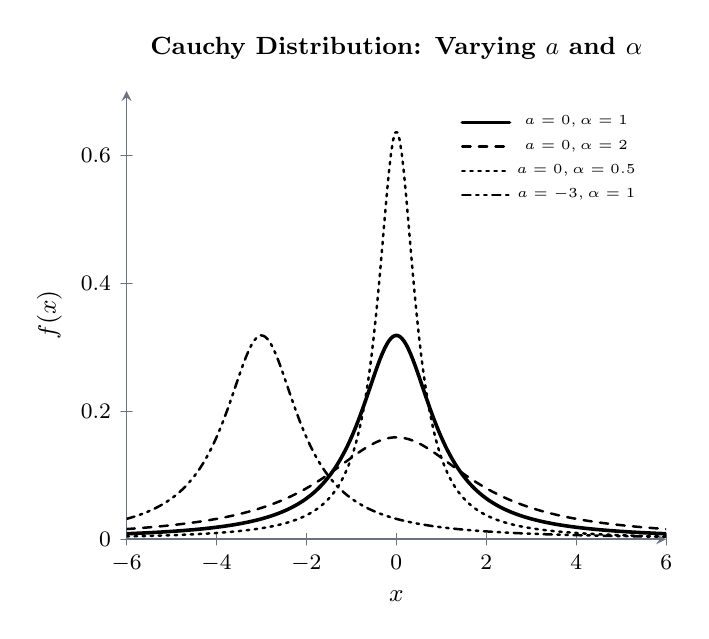
\begin{tikzpicture}
\begin{axis}[
    axis lines = left,
    xlabel = $x$,
    ylabel = {$f(x)$},
    domain = -6:6,
    samples = 250,
    ymin = 0, ymax = 0.7,
    xmin = -6, xmax = 6,
    legend pos = north east,
    legend style={draw=none, font=\tiny},
    title = {Cauchy Distribution: Varying $a$ and $\alpha$}
]

% 1. Standard Cauchy (a=0, alpha=1)
\addplot [black, ultra thick] {1 / (pi * (1 + x^2))};
\addlegendentry{$a=0, \alpha=1$}

% 2. Increased Scale (a=0, alpha=2)
\addplot [black, thick, dashed] {1 / (2 * pi * (1 + (x/2)^2))};
\addlegendentry{$a=0, \alpha=2$}

% 3. Decreased Scale (a=0, alpha=0.5)
\addplot [black, thick, dotted] {1 / (0.5 * pi * (1 + (x/0.5)^2))};
\addlegendentry{$a=0, \alpha=0.5$}

% 4. Shifted Location (a=-3, alpha=1)
\addplot [black, thick, dashdotdotted] {1 / (pi * (1 + (x+3)^2))};
\addlegendentry{$a=-3, \alpha=1$}

\end{axis}
\end{tikzpicture}
\caption{The Cauchy distribution under different parameters. Note how $\alpha$ controls the ``scale'' and $a$ controls the location.}
\end{figure}



\begin{remark}
The mean does not exist 
\[E(x)=\int^{\infty}_{-\infty}\dfrac{x}{\pi(1+(x-\theta)^2)}\, dx=H(x)\Bigg|_{-\infty}^{\infty}\quad\quad \text{diverges}\]
and 
\[E(x^2)=\int^{\infty}_{-\infty}\dfrac{x^2}{\pi (1+(x-\theta)^2)}\, dx\quad\quad \text{diverges}.\]
\end{remark}






\begin{exe}
Suppose that X has Cauchy $X\thicksim \operatorname{Cauchy}(1,0)$ distribution show that $E(X)$ does not exists.
\end{exe}




\subsection{The Weibull Distribution}
\vspace{-15pt}
The distribution is used in reliability and survival analysis to model the lifetime of an object, the lifetime of an organism or systems that fail at a constant rate, or systems that wear out as they age.

\begin{definition}[\textbf{Weibull Distribution $(X\thicksim \operatorname{Weibull}(\alpha, \beta)$}]
A Weibull random variable $X$ has p.d.f of form \[f_X(x) = \frac{\beta}{\alpha}\, x^{\beta - 1}\, e^{\left(-\frac{1}{\alpha}\right)x^{\beta}}\,, \quad\quad x> 0,\] with the scale parameter $\alpha > 0$ and  shape parameter $\beta > 0$.
\end{definition}


\begin{figure}[H]
\centering
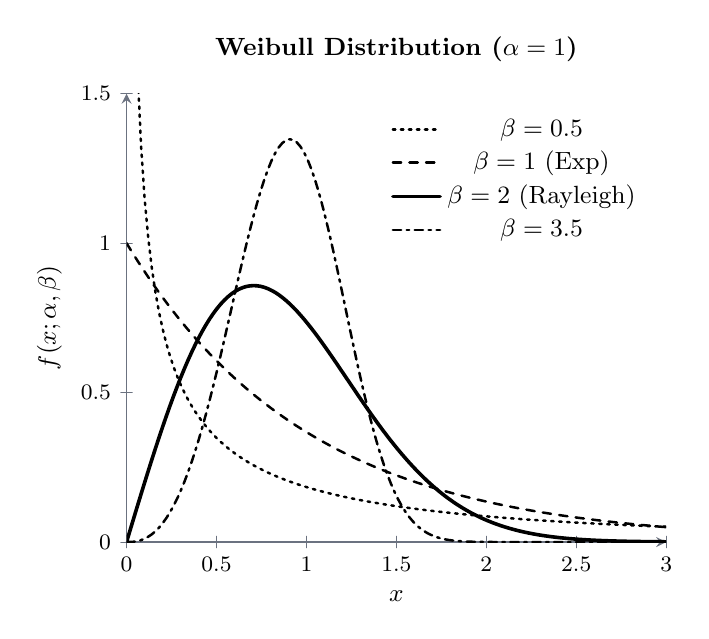
\begin{tikzpicture}
\begin{axis}[
    axis lines = left,
    xlabel = $x$,
    ylabel = {$f(x; \alpha, \beta)$},
    domain = 0:3,
    samples = 150,
    ymin = 0, ymax = 1.5,
    xmin = 0,
    legend pos = north east,
    legend style={draw=none, font=\small},
    title = {Weibull Distribution ($\alpha=1$)}
]

% beta = 0.5 (Decreasing failure rate)
\addplot [black, thick, dotted, restrict y to domain=0:2] 
    {(0.5/1) * x^(0.5-1) * exp(-(1/1)*x^0.5)};
\addlegendentry{$\beta=0.5$}

% beta = 1 (Exponential case - Constant failure rate)
\addplot [black, thick, dashed] 
    {(1/1) * x^(1-1) * exp(-(1/1)*x^1)};
\addlegendentry{$\beta=1$ (Exp)}

% beta = 2 (Rayleigh case - Increasing failure rate)
\addplot [black, ultra thick, solid] 
    {(2/1) * x^(2-1) * exp(-(1/1)*x^2)};
\addlegendentry{$\beta=2$ (Rayleigh)}

% beta = 3.5 (Normal-like shape)
\addplot [black, thick, dashdotted] 
    {(3.5/1) * x^(3.5-1) * exp(-(1/1)*x^3.5)};
\addlegendentry{$\beta=3.5$}

\end{axis}
\end{tikzpicture}
\caption{The Weibull distribution. Changing $\beta$ allows the model to shift from an exponential decay to a symmetric bell shape.}
\end{figure}

 
\begin{thm}
If $X \thicksim \operatorname{Weibull}(\alpha,\beta)$, then 
c.d.f is \[F_X(x) = P(X \leq x) = 1 - e^{-\frac{1}{\alpha}\, \beta^x}\, ,\]
the  mean is \[E(X) = \frac{\alpha}{\beta}\,\Gamma\left(\frac{1}{\beta}\right)\]
and the variance is \[\operatorname{Var}(X) = \alpha^2\left\{\frac{2}{\beta}\Gamma\left(\frac{2}{\beta}\right) - \left[\frac{1}{\beta}\, \Gamma\left(\frac{1}{\beta}\right)\right]^2\right\}.\]
\end{thm}


\subsection{Rayleigh Distribution}
\vspace{-15pt}
The Rayleigh distribution is a special case of the Weibull distribution (where the shape parameter is fixed), the only thing that changes here is the scale parameter $\alpha$.

\begin{definition}[\textbf{Rayleigh Distribution $(X\thicksim \operatorname{Rayleigh(\alpha)}$}]
A Rayleigh random variable $X$ with $\alpha > 0$ has p.d.f \[f_X(x) = \frac{2x\, e^{-\frac{x^2}{\alpha}}}{\alpha}\, , \quad\quad x > 0.\]
\end{definition}



\begin{figure}[H]
\centering
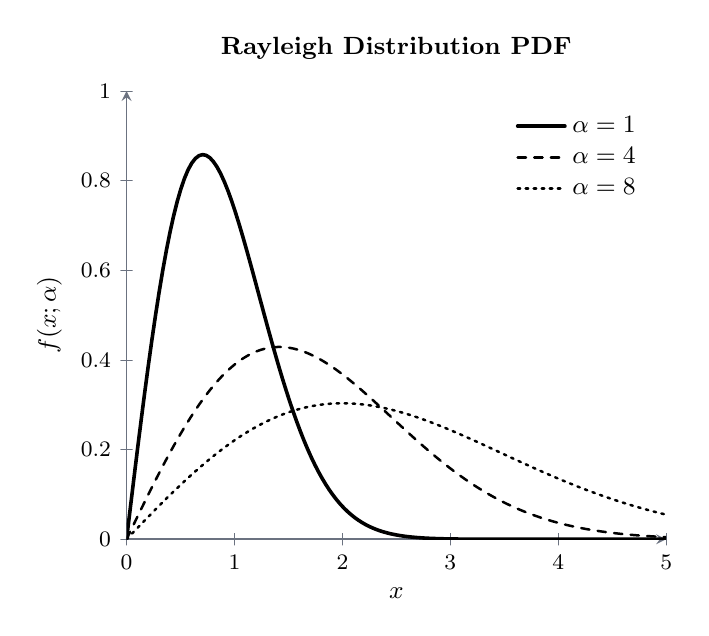
\begin{tikzpicture}
\begin{axis}[
    axis lines = left,
    xlabel = $x$,
    ylabel = {$f(x; \alpha)$},
    domain = 0:5,
    samples = 150,
    ymin = 0, ymax = 1.0,
    xmin = 0,
    legend pos = north east,
    legend style={draw=none, font=\small},
    title = {Rayleigh Distribution PDF}
]

% alpha = 1
\addplot [black, ultra thick, solid] {(2*x*exp(-x^2/1))/1};
\addlegendentry{$\alpha=1$}

% alpha = 4
\addplot [black, thick, dashed] {(2*x*exp(-x^2/4))/4};
\addlegendentry{$\alpha=4$}

% alpha = 8
\addplot [black, thick, dotted] {(2*x*exp(-x^2/8))/8};
\addlegendentry{$\alpha=8$}

\end{axis}
\end{tikzpicture}
\caption{The Rayleigh distribution. As $\alpha$ increases, the distribution spreads out and the peak shifts to the right.}
\end{figure}


\begin{exe}
Show that the mean of $X \thicksim \operatorname{Rayleigh}(\alpha)$ is \[E(X) = \frac{\sqrt{\alpha \pi}}{\pi}\] and Variance is \[\operatorname{Var}(X) = \frac{\alpha (4 - \pi)}{4}.\]
\end{exe}


\subsection{The Pareto Distribution}
\vspace{-15pt}
The Pareto distribution is a ``power-law'' distribution traditionally used to model the distribution of wealth and income. In this model, the parameter $\lambda$ represents the minimum value (such as a minimum wage), while $\kappa$ determines the shape of the distribution. Beyond economics, it is used to model the lifetime of objects with a mandatory warranty period $\lambda$, or the duration of events with a guaranteed minimum length $\lambda$, such as a labor strike.

\begin{definition}[\textbf{Pareto Distribution $X\thicksim\operatorname{Pareto}(\lambda, \kappa)$}]
A Pareto random variable $X$ with scale parameter $\lambda > 0$ and shape parameter $\kappa > 0$ has a p.d.f. given by:$$f\_X(x) = \frac{\kappa \lambda^{\kappa}}{x^{\kappa + 1}}, , \quad\quad x \geq \lambda.$$
\end{definition}







\begin{figure}[H]
\centering
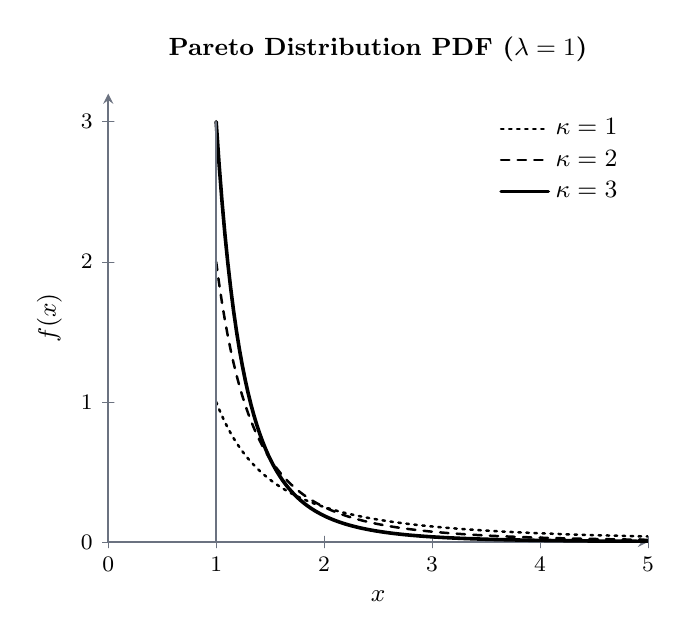
\begin{tikzpicture}
\begin{axis}[
    axis lines = left,
    xlabel = $x$,
    ylabel = {$f(x)$},
    domain = 1:5,
    samples = 150,
    ymin = 0, ymax = 3.2,
    xmin = 0, xmax = 5,
    legend pos = north east,
    legend style={draw=none, font=\small},
    title = {Pareto Distribution PDF ($\lambda = 1$)}
]

% kappa = 1
\addplot [black, thick, dotted] {1 * 1^1 / x^(1+1)};
\addlegendentry{$\kappa=1$}

% kappa = 2
\addplot [black, thick, dashed] {2 * 1^2 / x^(2+1)};
\addlegendentry{$\kappa=2$}

% kappa = 3
\addplot [black, ultra thick, solid] {3 * 1^3 / x^(3+1)};
\addlegendentry{$\kappa=3$}

% Vertical line to show the minimum value lambda
\draw [gray, thin] (axis cs: 1, 0) -- (axis cs: 1, 3);
\node [anchor=north] at (axis cs: 1, 0) {$\lambda$};

\end{axis}
\end{tikzpicture}
\caption{The Pareto distribution. Note that the density is zero for $x < \lambda$. Higher values of $\kappa$ lead to a faster decay in the probability of extreme values.}
\end{figure}


\begin{thm}
If $X\thicksim \operatorname{Pareto}(\alpha)$, then

the moment generating function is \[M_X(t) = \kappa (-\lambda t)^{\kappa}\Gamma(-\kappa,\lambda t),\]
the mean is \[E(X) = \frac{\kappa \lambda}{\kappa - 1}\,\,\, \text{for}\quad \kappa > 1,\] and the variance is \[\operatorname{Var}(X) = \frac{\kappa \lambda^2}{(\kappa - 1)^2(\kappa - 2)}\,\,\, \text{for}\quad \kappa > 2.\]
\end{thm}



\begin{remark}
\textbf{ }
\begin{enumerate}
\item The Pareto distribution is the mathematical backbone of the 80/20 rule (the Pareto Principle). For example, it often models how $80\%$ of a country's wealth is held by $20\%$ of the population.
\item Unlike the Normal or Gamma distributions, which can approach zero, the Pareto has a hard ``floor'' at $\lambda$. In many engineering applications, this represents the ``guaranteed'' life of a component before any failure is even possible.
\end{enumerate}
\end{remark}








\section{Cumulative Distribution Function (CDF)}
\begin{definition}
Let $X$ be a random variable with probability function $f_X(x)$, then cumulative distribution function (cdf) of $X$ denoted by $F_X(x)$ and is given by
$$F_X(t)=P(X\leq t)$$ 
specifically, calculated as
\[F_X(t)=
\begin{cases}
\sum\limits_{\{X:X\leq t\}}P(X=x) & \text{if}\quad X \quad\text{discrete}\\
\displaystyle{\int\limits_{\{X:X\leq t\}}}f_X(x)\, dx & \text{if}\quad X \quad\text{is continuous}\\
\end{cases}
\]
\end{definition}


\textbf{Fundamental Properties:}
\begin{enumerate}
\item $F_X(x)$ is a non-decreasing function.
\item $F_X(-\infty) = \lim_{x \to -\infty} F_X(x) = 0$.
\item $F_X(+\infty) = \lim_{x \to +\infty} F_X(x) = 1$.
\item $F_X(x)$ is right-continuous: $\lim_{h \to 0^+} F_X(x+h) = F_X(x)$.\\
\end{enumerate}


\begin{figure}[H]
\centering
\begin{minipage}{0.45\textwidth}
\centering
\begin{tikzpicture}[scale=0.9]
\draw[-Stealth] (-0.5,0) -- (4,0) node[right] {$x$};
\draw[-Stealth] (0,-0.5) -- (0,3) node[above] {$F_X(x)$};
\draw[blue, thick] (-0.5,0) -- (1,0);
\draw[blue, thick] (1,0.8) -- (2,0.8);
\draw[blue, thick] (2,1.8) -- (3,1.8);
\draw[blue, thick, ->] (3,2.5) -- (4,2.5);
\filldraw[blue] (1,0.8) circle (1.5pt);
\draw[blue] (1,0) circle (1.5pt);
\filldraw[blue] (2,1.8) circle (1.5pt);
\draw[blue] (2,0.8) circle (1.5pt);
\filldraw[blue] (3,2.5) circle (1.5pt);
\draw[blue] (3,1.8) circle (1.5pt);
\node at (0,2.5) [left] {$1$};
\end{tikzpicture}
\caption*{Discrete (Step Function)}
\end{minipage} \hfill
\begin{minipage}{0.45\textwidth}
\centering
\begin{tikzpicture}[scale=0.9]
\draw[-Stealth] (-1,0) -- (4,0) node[right] {$x$};
\draw[-Stealth] (0,-0.5) -- (0,3) node[above] {$F_X(x)$};
\draw[red, thick] plot [smooth, tension=0.7] coordinates {(0,0) (1.5,1.25) (3,2.5) (4,2.5)};
\draw[dashed] (0,2.5) -- (4,2.5);
\node at (0,2.5) [left] {$1$};
\end{tikzpicture}
\caption*{Continuous (Smooth)}
\end{minipage}
\end{figure}





\begin{example}Consider tossing a fair coin 3 times. Let $X \sim \operatorname{BIN}(3, 1/2)$.The p.m.f. is: $$f_X(x) = \binom{3}{x} \left(\frac{1}{2}\right)^3\quad \text{for} \quad x \in \{0, 1, 2, 3\}.$$
\[P(X = 0) = \frac{1}{8}\, ,\quad P(X = 1) = \frac{3}{8}\, ,\quad P(X = 2) = \frac{3}{8}\, , \quad P(X = 3) = \frac{1}{8}.\]
$F_X(t)=P(X\leq t)$

If $\, t < 0$ 
\[F_X(t)=P(X\leq t)=0.\]
If $\, 0\leq t<1$
\[F_X(t)=P(X\leq t)=P(X\leq 0)=P(X=0)=\frac{1}{8}.\]
If $\, 1 \leq t < 2$
\begin{align*}
P(1\leq t< 2) & = P(X\leq 1)=P(X=0,X=1)\\
              & = P(X=0)+P(X=1)\\
              & = \frac{1}{8}+\frac{3}{8}\\
              & = \frac{1}{2}.
\end{align*}
If $\, 2 \leq t < 3$
\begin{align*}
P(2 \leq t < 3) & = P(X\leq 2)\\
& = P(X = 0) + P(X = 1) + P(X = 2)\\
& = \frac{1}{8}+\frac{3}{8}+\frac{3}{8}\\
& =\frac{7}{8}.
\end{align*}
If $\, t\geq 3,$ $\,P(X\leq 3)=1$ since $$P(X=0)+P(X=1)+P(X=2)+P(X=3)=1.$$
Therefore, the c.d.f 
\[F_X(t)=
\begin{cases}
0 & \text{if}\hspace{0.3cm}t<0\\\\
\dfrac{1}{8} & \text{if}\hspace{0.3cm} 0\leq t<1\\\\
\dfrac{1}{2} & \text{if}\hspace{0.3cm} 1\leq t<2\\\\
\dfrac{7}{8} & \text{if}\hspace{0.3cm} 2\leq t<3\\\\
1 & \text{if} \hspace{0.3cm} t\geq 3\\
\end{cases}
\]
The plot
\begin{figure}[H]
\centering
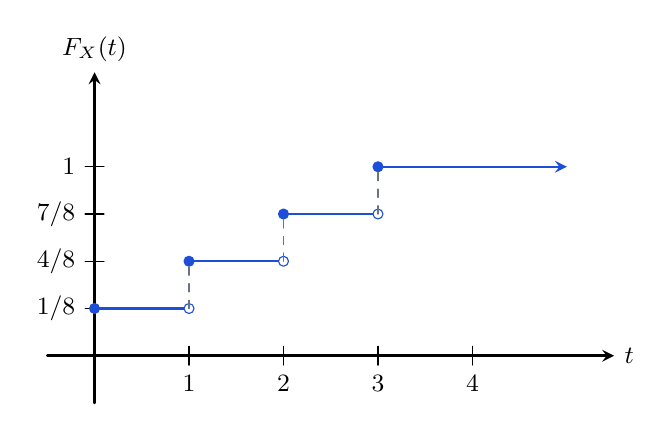
\begin{tikzpicture}[>=stealth, scale=1.2]
    % Axes
    \draw[->, thick] (-0.5,0) -- (5.5,0) node[right] {$t$};
    \draw[->, thick] (0,-0.5) -- (0,3) node[above] {$F_X(t)$};

    % Y-axis labels (Ticks)
    \foreach \y/\label in {0.5/{1/8}, 1.0/{4/8}, 1.5/{7/8}, 2.0/{1}} {
        \draw (0.1, \y) -- (-0.1, \y) node[left, font=\small] {$\label$};
    }

    % X-axis labels (Ticks)
    \foreach \x in {1, 2, 3, 4} {
        \draw (\x, 0.1) -- (\x, -0.1) node[below, font=\small] {$\x$};
    }

    % Step 1: 0 <= t < 1
    \draw[blue, thick] (0, 0.5) -- (1, 0.5);
    \filldraw[blue] (0, 0.5) circle (1.5pt); % Included
    \draw[blue, fill=white] (1, 0.5) circle (1.5pt); % Excluded

    % Step 2: 1 <= t < 2
    \draw[blue, thick] (1, 1.0) -- (2, 1.0);
    \filldraw[blue] (1, 1.0) circle (1.5pt);
    \draw[blue, fill=white] (2, 1.0) circle (1.5pt);
    \draw[gray, dashed] (1, 0.5) -- (1, 1.0); % Vertical jump line

    % Step 3: 2 <= t < 3
    \draw[blue, thick] (2, 1.5) -- (3, 1.5);
    \filldraw[blue] (2, 1.5) circle (1.5pt);
    \draw[blue, fill=white] (3, 1.5) circle (1.5pt);
    \draw[gray, dashed] (2, 1.0) -- (2, 1.5);

    % Step 4: t >= 3
    \draw[blue, thick, ->] (3, 2.0) -- (5, 2.0);
    \filldraw[blue] (3, 2.0) circle (1.5pt);
    \draw[gray, dashed] (3, 1.5) -- (3, 2.0);
\end{tikzpicture}
\caption{Graph of $F_X(t)$}
\end{figure}
\end{example}





\begin{example}
Let the pdf of a random variable $X$ be $$f_X(x)=\dfrac{x+1}{8},\quad 2<x<4.$$
Find the c.d.f and plot it.
\end{example}
\begin{proof}[\textbf{\textit{Solution}}]
$$F_X(t)=P(X\leq t)=\displaystyle{\int\limits_{\{X:X\leq t\}}}f_X(x)dx$$

If $\, t \leq 2$, \[F_X(t)=0.\]

If $t$ is such $2<t<4$
\begin{align*}
F_X(t)=P(X\leq t) & = \int^t_2f_X(x)\, dx\\
& =\int^t_2\frac{x+1}{8}dx\\
& = \frac{(x+1)^2}{8}\Big|^t_2\\
& = \frac{(t+1)^2-9}{16}.
\end{align*}
If $\, t\geq 4$,
\begin{align*}
F_X(t) & = P(X\leq t)\\
& = \int^t_2f_X(x)\, dx+\int^t_4f_X(x)\,dx\\
& = 1+0\\
& = 1.
\end{align*}


Therefore the c.d.f
\[F_X(t)=
\begin{cases}
0 & \text{if}\hspace{0.5cm} t\leq 2\\
\dfrac{(t+1)^2-9}{16} & \text{if}\hspace{0.5cm} 2<t<4\\
1 & t\geq 4\\
\end{cases}
\]

The plot
\begin{figure}[H]
\centering
\begin{tikzpicture}[>=stealth]
\begin{axis}[
    axis lines = left,
    xmin=1.5, xmax=4.5,
    ymin=0, ymax=1.05,
    xlabel={$t$},
    ylabel={$F_X(t)$},
    samples=200,
    domain=2:4,
    width=10cm,
    height=6cm,
    thick,
    ticks=none
]

% F(x)=0 for x<=2
\addplot[thick] coordinates {(1.5,0) (2,0)};

% CDF curve
\addplot[thick] {(x^2)/16 + x/8 - 0.5};


% F(x)=1 for x>=4
\addplot[thick] coordinates {(4,1) (4.5,1)};

% Points
\addplot[only marks, mark=*, mark size=1.5pt] coordinates {(2,0) (4,1)};

\end{axis}
\end{tikzpicture}
\caption{c.d.f $X$}
\end{figure}
\end{proof}

























\begin{remark}
\textbf{ }
\begin{enumerate}
\item In the case where $X$ is discrete with possible values $x_1,x_2,x_3,\cdots$ $$f_X(x_j)=P(X=x_j)=F_X(x_j)-F_X(x_{j-1})$$

For continuous random variable
\begin{align*}
P(a<X<b)& = \int^a_bf_X(x)dx\\
        & = \int^b_{-\infty}f_X(x)dx-\int^a_{-\infty}f_X(x)dx\\
        & = F_X(b)-F_X(a)
\end{align*}

also, $P(a\leq X< b)=P(a\leq X\leq b)=P(a<X\leq b)$
\item From fundamental theorem of calculus, it follows that if $F_X(t)$ is differentiable then $$f_X(x)=\dfrac{d}{dx}F_X(x).$$
\item For discrete random variables $X$ with possible values in ascending order $x_1,x_2,x_3,\cdots$ then $$F_X(t)=P(X\leq t)=\sum\limits^k_{j=1}P(X=x_j)$$
where $k$ is such that $x_{k-1}<t\leq x_k$.

\[F_X(t)=
\begin{cases}
0, & t<x_1\\
\sum\limits^k_{j=1}P(X=x_j) &\\
1&\text{if}\hspace{0.3cm}t>x_N,\hspace{0.3cm}\text{where}\hspace{0.3cm}x_N\hspace{0.3cm} \text{is the largest}\\
\end{cases}
\]
\item If $X$ is continuous random variable with pdf having support in the interval $(u,v)$. i.e $f_X(x)$ is defined on $(u,v)$ and 0 else where
\[ F_X(t)=
\begin{cases}
0 & \text{if}\hspace{0.3cm} t<u\\
\displaystyle{\int^t_uf_X(x)dx} & \text{if}\hspace{0.3cm} u<t<v\\
1 & \text{if}\hspace{0.3cm} t\geq v\\
\end{cases}
\]
\end{enumerate}
\end{remark}



\begin{example}
Suppose a random variable has the following probability mass functions: \[P(X = 1) = \frac{1}{2}\, , \quad P(X = 2) = \frac{1}{4}\, ,\quad P(X = 3) = \frac{1}{8}\, , \quad P(X = 4) = \frac{1}{8}.\] Find the c.d.f of the random variable $X$ and use it to find $P(X \leq 1)\, , \quad P(1 < X < 3)$ and $P(1\leq X \leq 3)$.
\end{example}

\begin{proof}[\textbf{\textit{Solution}}]
The c.d.f
\begin{align*}
F_X(t) & = \begin{cases}
0, & t < 1\\
\frac{1}{2}, & 1\leq t < 2\\
\frac{3}{4}, & 2\leq t < 3\\
\frac{7}{8}, & 3 \leq < 4\\
1, & t\geq 4.
\end{cases}
\end{align*}
The $P(X\leq 1)$ is \[P(X\leq 1) = F(1^+)  = \frac{1}{2}.\]
The $P(1 < X < 3)$ is
\begin{align*}
P(1 < X < 3) & = F(3^-) - F(1^+)\\
& = \frac{3}{4}-\frac{1}{2}\\
&=\frac{1}{4}.
\end{align*}
The $P(1\leq X \leq 3)$ is 
\begin{align*}
P(1 \leq X \leq 3) & = F(3^+) - F(1^-)\\
& = \frac{7}{8}-0\\
& = \frac{7}{8}.
\end{align*}
\end{proof}



\begin{example}
Use the c.d.f of 
$$f_X(x)=\dfrac{x+1}{8}\, ,\quad 2<x<4$$
to find the following probabilities: 
Using Cdf find:
\begin{enumerate}
\item[(i).] $P(1< X <2\frac{1}{2})$
\item[(ii).] $P(2\frac{1}{2}< X \leq 3)$
\item[(iii).] $P(3< X <5)$
\end{enumerate}
\end{example}

\begin{proof}[\textbf{\textit{Solution}}]
The c.d.f is given by
\[F_X(t)=
\begin{cases}
0, & t<2\\
\dfrac{(t+1)^2-9}{16}, & 2\leq t<4\\
1, & t\geq 4\\
\end{cases}
\]

Then 
\begin{align*}
P\left(1<X<2\frac{1}{2}\right) & =F_X\left(\frac{5}{2}\right)-F_X(1)\\
                              & = \frac{(2\frac{1}{2}+1)^2-9}{16}-0\\
                              & = \frac{\dfrac{49}{4}-9}{16}\\
                              & = \frac{49-36}{64}\\
                              & = \frac{13}{64}.
\end{align*}
Also
\begin{align*}
P\left(2\frac{1}{2} < X < 3\right) & = F_X(3) - F_X\left(\frac{5}{2}\right)\\
& = \frac{(3 + 1)^2 -9}{16}-\frac{13}{64}\\
& = \frac{7}{16}-\frac{13}{64}\\
& =\frac{15}{62}.
\end{align*}
And
\begin{align*}
P(3<X<5) &=F_X(5)-F_X(3)\\ 
&=1-\left(\frac{4^2-9}{16}\right)\\
& =1-\frac{7}{16}\\
&=\frac{9}{16}.
\end{align*}
\end{proof}














\begin{thm}
$X\thicksim N(\mu,\sigma^2)$ is read as $X$ is distributed as a normal with mean $\mu$ and variance $\sigma^2$.
If $$Z=\dfrac{X-\mu}{\sigma},$$ then $Z$ is distributed as normal with mean 0 and variance 1 and is known as standard normal, notation $Z\thicksim N(0,1)$.
\end{thm}


\begin{note}
Normal variable is usually referred to as Gaussian Distribution.
\end{note}

The c.d.f for the standard normal
$$\Phi(z)=\int^z_{-\infty}\frac{e^{\displaystyle{-\frac{1}{2}v^2}}}{\sqrt{2\pi}}\, dv$$


$$\Phi(-1.11)=\int^{-1.11}_{-\infty}\frac{e^{\displaystyle{-\frac{1}{2}t^2}}}{\sqrt{2\pi}}\, dt$$

% DIAGRAM 16

\begin{figure}[H]
\centering
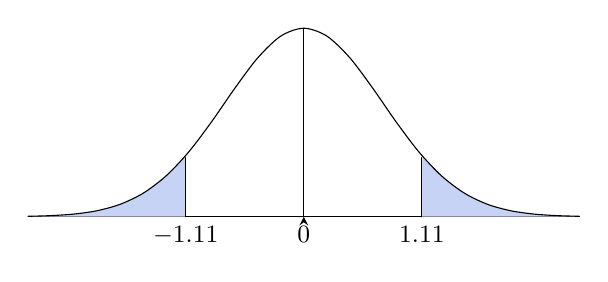
\begin{tikzpicture}[->,>=stealth]
\draw[-](-3.5,0)--(3.5,0);
\draw[-](0,0)--(0,2.39);
% tex4ht cannot convert TikZ patterns - the figure came out blank on the
% web. A solid translucent fill shows the same region and reads better.
\path[fill=blue!25,smooth,domain=1.5:3.5,variable=\x]plot(\x,{6*1/sqrt(2*pi)*exp(-1/2*\x*\x)})--(3.5,0)--(1.5,0)--(1.5,0.75);
\path[fill=blue!25,smooth,domain=-3.5:-1.5,variable=\x]plot(\x,{6*1/sqrt(2*pi)*exp(-1/2*\x*\x)})--(-1.5,0.75)--(-1.5,0)--(-3.5,0);
% The picture sets [->] as the default for every path, which put an
% arrowhead on the peak of the bell curve. Force this one to be plain.
\draw[-,smooth,domain=-3.5:3.5,variable=\x]plot(\x,{6*1/sqrt(2*pi)*exp(-1/2*\x*\x)});
\draw[-](1.5,0.75)--(1.5,0);
\draw[-](-1.5,0)--(-1.5,0.75);
\draw(-1.5,0)node[below]{$-1.11$}
(1.5,0)node[below]{1.11}
(0,0)node[below]{0};
\end{tikzpicture}
\caption{By symmetry, the lower tail below $z=-1.11$ has the same area as the upper tail above $z=1.11$; hence $\Phi(-1.11)=1-\Phi(1.11)$.}
\end{figure}







\begin{align*}
\Phi(-1.11) & = 1-\Phi(1.11)\\
            & = 1-0.8643\\
            & = 0.1357\\
\end{align*}


$P(z\geq 2)=P(z>2)$


% DIAGRAM 17


\begin{figure}[H]
\centering
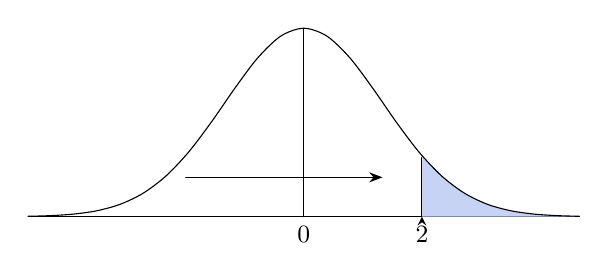
\begin{tikzpicture}[->,>=stealth]
\draw[-](-3.5,0)--(3.5,0);
\draw[-](0,0)--(0,2.39);
% tex4ht cannot convert TikZ patterns - the figure came out blank on the
% web. A solid translucent fill shows the same region and reads better.
\path[fill=blue!25,smooth,domain=1.5:3.5,variable=\x]plot(\x,{6*1/sqrt(2*pi)*exp(-1/2*\x*\x)})--(3.5,0)--(1.5,0)--(1.5,0.75);
% The picture sets [->] as the default for every path, which put an
% arrowhead on the peak of the bell curve. Force this one to be plain.
\draw[-,smooth,domain=-3.5:3.5,variable=\x]plot(\x,{6*1/sqrt(2*pi)*exp(-1/2*\x*\x)});
\draw[-](1.5,0.75)--(1.5,0);
\draw(0,0)node[below]{0}
(1.5,0)node[below]{2};
\draw[-Stealth](-1.5,0.5)--(1,0.5);
\end{tikzpicture}
\caption{$P(Z\geq 2)$ is the area in the upper tail beyond $z=2$.}
\end{figure}

\begin{align*}
P(z\geq 2) & = 1-P(z\leq 2)\\
           & = 1-\Phi(2)\\
           & = 1-0.9772\\
           & = 0.0228
\end{align*}
\begin{align*}
P(-1.02<z<1.96) & = \Phi(1.96)-\Phi(-1.02)\\
                & = \Phi(1.96)-(1-\Phi(1.02))\\
                & = \Phi(1.96)+\Phi(1.02)-1\\
                & = 0.9750+0.8461-1\\
                & = 0.8211
\end{align*}


\begin{example}
The Rock well hardness of a metal specimen is determined by pressing the surface of the specimen with hardened point, and then measuring the depth of penetration. The hardness of an alloy is normally distributed with mean 70 units and standard deviation 3 units.

\begin{enumerate}
\item If a specimen is acceptable only if its hardness is between 66 and 74 units. What is the probability that a randomly chosen specimen is acceptable?
\begin{proof}[\textbf{\textit{Solution}}]
 $P(66\leq x\leq 74)= $?
\begin{align*}
P\left(\frac{66-70}{3}< Z <\frac{74-70}{3}\right) & = P\left(-\frac{4}{3}< Z <\frac{4}{3}\right)\\
                                               & = 2P\left(0 < Z <\frac{4}{3}\right)\\
                                               & = 2\left[\Phi\left(\frac{4}{3}\right)-\Phi(0)\right]\\
                                               & = 2[0.9082-0.5000]\\
                                               & = 0.8164
\end{align*}
\end{proof}




\item If the acceptable range is $70\pm c$, for what value of $c$ would $95\%$ of all the specimens to be acceptable?
\begin{proof}[\textbf{\textit{Solution}}]
\[P\left(-\frac{c}{3}< Z <\frac{c}{3}\right)  = 0.95\]
\[2P\left(0<z<\frac{c}{3}\right)  = 0.95\]
\[\implies P\left(0< Z <\frac{c}{3}\right)  = 0.475\]
Therefore
\[\frac{c}{3} =1.960\, \, \implies\,\,  c=3\times 1.960=5.880\]






\begin{figure}[H]
\centering
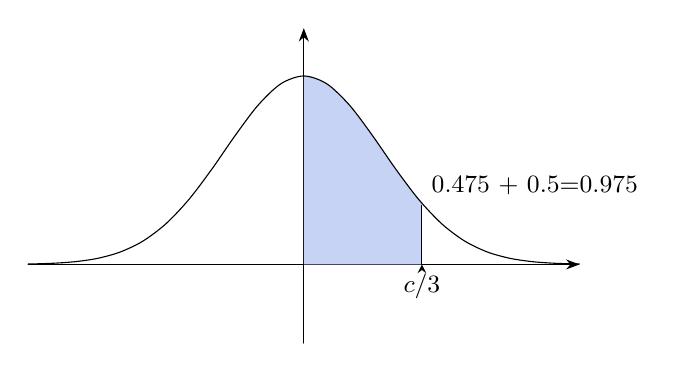
\begin{tikzpicture}[->,>=stealth]
\draw[-Stealth](-3.5,0)--(3.5,0);
\draw[-Stealth](0,-1)--(0,3);
% tex4ht cannot convert TikZ patterns - the figure came out blank on the
% web. A solid translucent fill shows the same region and reads better.
\path[fill=blue!25,smooth,domain=0:1.5,variable=\x]plot(\x,{6*1/sqrt(2*pi)*exp(-1/2*\x*\x)})--(1.5,0.75)--(1.5,0)--(0,0)--(0,2.39);
% The picture sets [->] as the default for every path, which put an
% arrowhead on the peak of the bell curve. Force this one to be plain.
\draw[-,smooth,domain=-3.5:3.5,variable=\x]plot(\x,{6*1/sqrt(2*pi)*exp(-1/2*\x*\x)});
\draw[-](1.5,0.75)--(1.5,0);
\draw(1.5,1)node[right]{0.475 + 0.5=0.975}
(1.5,0)node[below]{$c/3$};
\end{tikzpicture}
\caption{$P(0<Z<c/3)=0.475$, so the area to the left of $c/3$ is $0.975$.}
\end{figure}
\end{proof}
\end{enumerate}
\end{example}

















\section{Markov's and Chebyshev's Inequality}
\vspace{-15pt}
The primary value of Markov’s and Chebyshev’s inequalities lies in their ability to provide rigorous probability bounds when our knowledge of a distribution is limited. Specifically, these inequalities allow us to estimate the likelihood of events when we know only the mean, or both the mean and variance, of a random variable. (i.e underlying distribution is either unknown or too complex to compute directly.)


\begin{lem}[\textbf{Markov's Inequality}]
Let $X$ be a non-negative random variable having a finite mean and $t$ be a positive real number then $$P(X\geq t)\leq \frac{E(X)}{t}.$$
\end{lem}

\begin{proof}
Define a random variable $Y$ as follows 
\[\begin{cases}
y=0, &\text{if}\quad x<t\\
y=t, &\text{if}\quad x\geq t
\end{cases}\]
$y$ is discrete. Then
\[f_Y(y)=
\begin{cases}
0, & P(x<t)\\
t, & P(x\geq t)
\end{cases}\]
Thus \[X \geq Y\]
\[E(X)  \geq E(Y)=0\,P(X<t)+t\,P(X\geq t)\]
\[E(X) \geq tP(X\geq t)\] 
\[\frac{E(X)}{t}\geq P(X\geq t)\]
\[ P(X\geq t) \leq \frac{E(X)}{t}.\]
\end{proof}



\begin{thm}[\textbf{Chebyshev's Inequalit}]
Let $X$ be a random variable with mean $\mu$ and finite variance $\sigma^2$, then for any real number $t>0$ \[P(|X-\mu|\geq t)\leq \frac{\sigma^2}{t^2}\]
or  \[P(|X-\mu|<t)>1-\frac{\sigma^2}{t^2}.\]
\end{thm}

\begin{proof}
Since $(X - \mu)^2 \geq 0$, we apply the Markov's inequality to obtain 
\[P\left((X-\mu)^2\geq t^2\right)  \leq \frac{E(X-\mu)^2}{t^2}=\frac{\sigma^2}{t^2}\]
That is  \[P\left((X-\mu)\geq t^2\right)  \leq \frac{\sigma^2}{t^2}\]
Now, since  $(X-\mu)^2\geq t^2  \iff |X-\mu|\geq t$. Therefore, \[P(|X-\mu|\geq t) \leq \frac{\sigma^2}{t^2}.\]
\end{proof}






\begin{remark}
\textbf{ }
\begin{enumerate}
\item[i)] \textbf{The Complementary Nature of the Bound:}The event $|X-\mu| \geq t$ represents the ``tails'' of the distribution—values that are far from the mean.$$ |X-\mu| \geq t \iff (X \geq \mu + t) \text{ or } (X \leq \mu - t) $$
\item[ii)] \textbf{Visualizing the Upper and Lower Bounds:}
If we set $t = k\sigma$, Chebyshev's inequality tells us:
\begin{itemize}
    \item The probability in the \textbf{shaded tails} (at most distance $k\sigma$ away) is at most $\frac{1}{k^2}$.
    \item The probability in the \textbf{shaded center} (within distance $k\sigma$) is at least $1 - \frac{1}{k^2}$.
\end{itemize}

\vspace{0.5cm}
\textbf{Case A: Probability in the Tails (Maximum $\frac{1}{k^2}$)}
\begin{figure}[H]
\centering
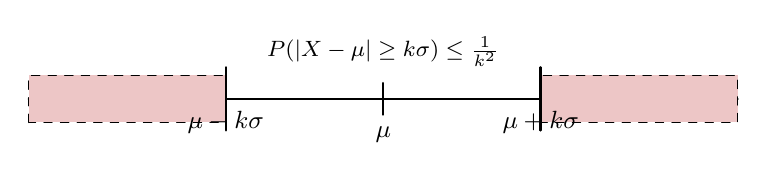
\begin{tikzpicture}[>=stealth]
    % Main Axis
    \draw[thick] (-4.5,0) -- (4.5,0);
    % Shaded Tails
    \fill[red!25] (-4.5,-0.3) rectangle (-2,0.3);
    \fill[red!25] (2,-0.3) rectangle (4.5,0.3);
    % Boundary Lines
    \draw[thick] (-2,-0.4) -- (-2,0.4) node[below=12pt] {$\mu - k\sigma$};
    \draw[thick] (2,-0.4) -- (2,0.4) node[below=12pt] {$\mu + k\sigma$};
    \draw[thick] (0,-0.2) -- (0,0.2) node[below=12pt] {$\mu$};
    % Dashed Rectangles
    \draw[dashed] (-4.5,-0.3) rectangle (-2,0.3);
    \draw[dashed] (2,-0.3) rectangle (4.5,0.3);
    \node at (0,0.6) {\footnotesize $P(|X-\mu| \geq k\sigma) \leq \frac{1}{k^2}$};
\end{tikzpicture}
\end{figure}

\vspace{0.8cm}
\textbf{Case B: Probability in the Center (Minimum $1 - \frac{1}{k^2}$)}
\begin{figure}[H]
\centering
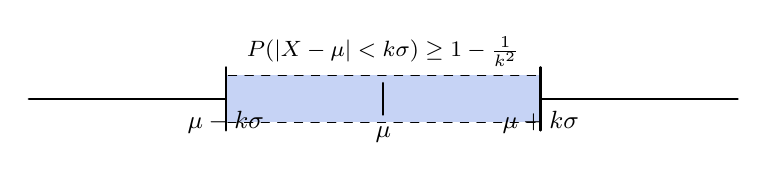
\begin{tikzpicture}[>=stealth]
    % Main Axis
    \draw[thick] (-4.5,0) -- (4.5,0);
    % Shaded Center
    \fill[blue!25] (-2,-0.3) rectangle (2,0.3);
    % Boundary Lines
    \draw[thick] (-2,-0.4) -- (-2,0.4) node[below=12pt] {$\mu - k\sigma$};
    \draw[thick] (2,-0.4) -- (2,0.4) node[below=12pt] {$\mu + k\sigma$};
    \draw[thick] (0,-0.2) -- (0,0.2) node[below=12pt] {$\mu$};
    % Dashed Rectangle
    \draw[dashed] (-2,-0.3) rectangle (2,0.3);
    \node at (0,0.6) {\footnotesize $P(|X-\mu| < k\sigma) \geq 1 - \frac{1}{k^2}$};
\end{tikzpicture}
\end{figure}
\end{enumerate}
\end{remark}










\begin{example}
From a quick analysis of records a materials control manager estimates that the mean and standard deviation of the ``lead time'' required in ordering a small value are 8 days and 1.5 days respectively. The manager is willing to assume the mean and variance to be absolutely correct. The manager would like to determine a time interval such that the probability is at least $\frac{8}{9}$  that the order will be received during the time interval.
\end{example}

\begin{proof}[\textbf{\textit{Solution}}]
$\mu = 8, \,\, \sigma = 1.5$ and \[P(|X-\mu|<k\sigma) \geq 1-\frac{1}{k^2}=\frac{8}{9}\,\,\implies\,\, k=3.\]
Then 
\[(\mu-k\sigma,\mu+k\sigma)= (8-3(1.5),8+3(1.5)) =(3.5,12.5).\]
\end{proof}




\begin{example}
Suppose we want the number of items produced in a factory during a week is a random variable with mean 500.
\begin{enumerate}
\item What can be said about the probability that the weeks production will be at least 1000?
\begin{proof}[\textbf{\textit{Solution}}]
$\mu=500$, $P(X\geq 1000)$ by Markov's inequality we get $$P(X\geq 1000)\leq \frac{E(X)}{1000}=\frac{500}{1000}=\frac{1}{2}.$$
\end{proof}


\item If the variance of a week's production is known to be 100, what can be said about the probability that this week's production will be between 420 and 580?
\begin{proof}[\textbf{\textit{Solution}}]
$\mu=500$, $\sigma =10$
\[P(|X-\mu|<k\sigma)\geq 1-\frac{1}{k^2}\] rewriting the expression 
\[P(\mu -k\sigma < X < \mu + k\sigma)\geq 1-\frac{1}{k^2}\]
but we have $P(420 < X < 580)$
therefore
$$500-k(10)=420\,\,\implies k=8$$ 
$$500+k(10)=580\,\,\implies k=8.$$
\end{proof}
\end{enumerate}
\end{example}







\chapter{Jointly Distributed Random Variables}
\section{Introduction}
\vspace{-16pt}
The study of random variables and their probability distributions so far has been restricted to one-dimensional sample spaces. There are many situations where we may want to describe  several random variables. For example we might measure amount of precipitate $X$ and the volume $Y$ of a gas released from a controlled chemical giving rise to two-dimensional space. At this level of the course we will concentrate on two variables.



\section{Joint Distributions}
\vspace{-14pt}
\begin{definition}
Let $X$ and $Y$ be discrete random variables, a formula or table listing all the possible values of $X$ and $Y$ together with the associated probabilities is called a joint probability distribution of $X$ and $Y$ denoted by $f_{X,Y}(x,y)$ and is given \[f_{X,Y}(x,y)=P(X=x, Y=y)\] and \[\sum_x\sum_yf_{X,Y}(x,y)=\sum_x\sum_yP(X=x, Y=y).\]
\end{definition}







\begin{example}
Two refills for a ball point pen are selected at random from a box that contains 3 blue refills, 2 red refills and 3 green refills. Let $X$ be the number of blue refills and $Y$ be the number of red refills selected. Find the joint distribution of $X$ and $Y$.
\end{example}


\begin{proof}[\textit{Solution.}]
Possible values of $X$ are: $0,\, 1,\, 2$ and $Y$ are $0,\, 1,\, 2.$
\begin{table}[H]
\centering
\begin{tabular}{c|ccc}
 &\multicolumn{3}{c}{$Y$}\\
 $X$&0&1&2\\
\hline
0& $\frac{3}{28}$ & $\frac{6}{28}$ & $\frac{1}{28}$\\
&&&\\
1&$\frac{9}{28}$ & $\frac{6}{28}$ & 0\\
&&&\\
2 & $\frac{3}{28}$ & 0 & 0\\
\hline 
\end{tabular}
\end{table}

\[P(X=0, Y=0) =\frac{\binom{3}{0}\,\binom{2}{0}\,\binom{3}{2}}{\binom{8}{2}}=\frac{3}{28}\]
\[P(X=0, Y=1) =\frac{\binom{3}{0}\,\binom{2}{1}\, \binom{3}{1}}{\binom{8}{2}}=\frac{2\times 3}{28}=\frac{6}{28}\]
Therefore, the general formula is:
\[f_{X,Y}(x,y) =P(X=x, Y=y)=\frac{\binom{3}{x}\,\binom{2}{y}\binom{3}{2-x-y}}{\binom{8}{2}}.\]
\end{proof}


\begin{definition}
Let $X$ and $Y$ be continuous random variables with joint range $B$ in the Euclidean space, then $f_{X,Y}(x,y)$ the joint probability function has the following properties:
\begin{enumerate}
\item[a).] $f_{X,Y}(x,y)\geq 0\,$ for  $\,x,\, y\in B$
\item[b).]\quad $\displaystyle{\iint\limits_Bf_{X,Y}(x,y)\,dx\, dy=\iint\limits_Bf_{X,Y}(x,y)\,dy\,dx=1}$
\end{enumerate}
\end{definition}




\begin{remark}
The joint p.d.f for two continuous random variables lying in a specified region 
\[P(a<X<b, c<Y<d)=\int^b_a\int^d_cf_{X,Y}(x,y)\, dy\, dx=\int^d_c\int^b_af_{X,Y}(x,y)dx\,dy\]
\end{remark}


\begin{example}
Suppose that the variation in two continuous random variables, $X$ and $Y$, can be modeled by the joint p.d.f $f_{X,Y}(x,y) = cxy$, for $0 < y < x < 1$. Find $c$.
\end{example}

\begin{proof}[\textit{Solution.}] 
By inspection, (a) in the definition 3.1.3, $f_{X,Y}(x,y)$ will be nonnegative as long as $c\geq 0$.
\[\iint_{B}cxy\, dy\, dx = 1\quad \implies\quad\int^1_0\int^x_0cxy\, dy \, dx = 1\]
\[c\int^1_0\left[\frac{y^2}{2}\right]^x_0\, dx =  1\]
\[c\int^1_0\frac{x^3}{2}\, dx = 1\]
\[c\left[\frac{x^4}{8}\right]^1_0 = 1\]
\[\frac{c}{8} = 1.\]
Therefore, $c = 8$.
\end{proof}



\begin{example}
Let $X$ and $Y$ be random variables with a joint p.d.f 
\[f_{X,Y}(x,y)=x+y\, ,\quad x\in (0,1),\quad y\in (0,1).\]
Find:
\begin{enumerate}
\item[(i).] Show that $f_{X,Y}(x,y)$ is indeed a joint p.d.f.
\begin{proof}[\textit{Solution.}]
We show that $\iint_B f_{X,Y}(x,y) = 1.$
\begin{align*}
\int^1_0\int^1_0(x+y)\, dx\, dy & = \int^1_0\left[\frac{x^2}{2}+xy\right]^1_0\, dy\\
                                                       & = \int^1_0\left(\frac{1}{2}+y\right)dy\\
                                                       & = \left[\frac{1}{2}y+\frac{y^2}{2}\right]^1_0\\
                                                       & = 1.
\end{align*}
\end{proof}


\item[(ii).] Find $P(x+y<1)$.
\begin{proof}[\textit{Solution}.]
The region of integration is the area below the line $x + y = 1$.

\begin{figure}[H]
\centering
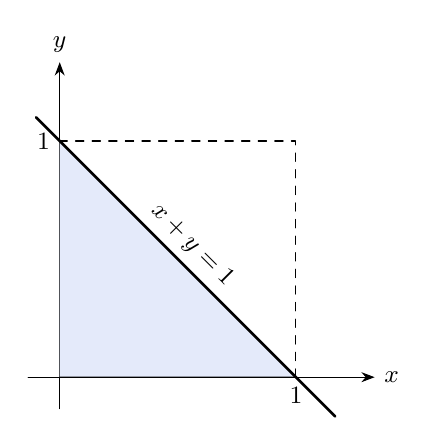
\begin{tikzpicture}
\draw[-Stealth](-0.4,0)--(4,0)node[right]{$x$};
\draw[-Stealth](0,-0.4)--(0,4)node[above]{$y$};
\draw[fill=blue!12](0,0)--(3,0)--(0,3);
\draw[smooth,domain=-0.3:3.5,variable=\x,thick]plot(\x,-\x+3);
\draw(0,3)--node[above,sloped]{$x + y = 1$}(3,0);
\draw(0,3)node[left]{1}
(3,0)node[below]{1};
\draw[dashed](3,0)--(3,3)--(0,3);
\end{tikzpicture}
\caption{The region of integration for $P(X+Y<1)$: the triangle below the line $x+y=1$ in the first quadrant.}
\end{figure}
\begin{align*}
P(X+Y <1) & = \int^1_0\int^{1-y}_0(x+y)\, dx\, dy
          = \int^1_0\left[\frac{x^2}{2}+xy\right]^{1-y}_0dy\\
%         & = \int^1_0\left(\frac{(1-y)^2}{2}+(y-y^2)\right)dy\\
         & = \int^1_0\left(\frac{1-2y+y^2}{2}+y-y^2\right)\, dy\\
         & = \frac{1}{2}\int^1_0(1-y^2)dy\\
        & = \frac{1}{3}.
\end{align*}
Therefore, $P(X + Y < 1) = \frac{1}{3}.$
\end{proof}

\item[(iii).] (\textit{Exercise}) Find $P\left(X+Y>1\frac{1}{2}\right)$
\end{enumerate}
\end{example}



\begin{exe}
A study claims that the daily number of hours, $X$, a teenager watches television and the daily number of hours, $Y$, he works on his homework are approximated by the joint p.d.f \[f_{X,Y}(x,y) = xye^{-(x+y)}\, , \quad x > 0, \quad y > 0.\]
What is the probability that a teenager chosen at random spends at least twice as much time watching television as he does working on this homework?
\end{exe}


\begin{proof}[\textit{Solution}.]
The region, $B$, in the $xy-$plane corresponding to the event ``$X \geq 2Y$''.

\begin{figure}[H]
\centering
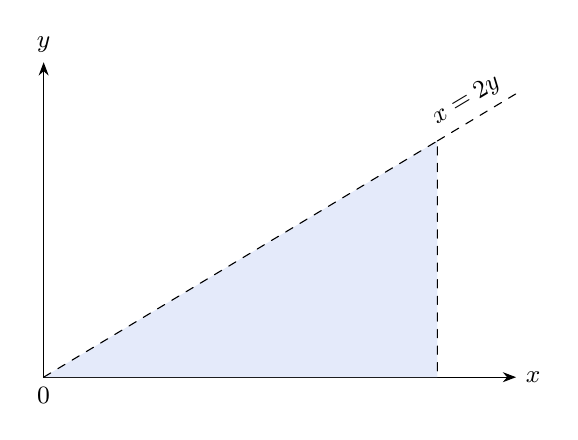
\begin{tikzpicture}
\draw[-Stealth](0,0)--(6,0)node[right]{$x$};
\draw[-Stealth](0,0)--(0,4)node[above]{$y$};
\draw[fill=blue!12,dashed](0,0)--(5,3)--(5,0);
\draw[dashed](5,3)--node[above,sloped]{$x = 2y$}(6,3.6);
\draw(0,0)node[below]{0};
\end{tikzpicture}
\caption{The event $X\geq 2Y$: the region of the $xy$-plane on or below the line $x=2y$.}
\end{figure}

\[P(2Y \leq X) = \int_0^{\infty}\int_0^{\frac{x}{2}} xye^{-(x + y)}\, , \, dy\, dx\]
We can write
\begin{align*}
P(X \leq 2Y) & = \int^{\infty}_0 xe^{-x}\left[\int^{x/2}_0 y e^{-y}\, dy\right]\, dx\\
& = \int^{\infty}_0xe^{-x}\left[1- \left(\frac{x}{2} + 1\right)e^{-x/2}\right]\, dx\\
& = \int^{\infty}_0 xe^{-x}\, dx - \frac{1}{2}\int_0^{\infty}e^{-3x/2}\, dx - \int^{\infty}_0xe^{-3x/2}\, dx\\
& = 1 - \frac{16}{54}-\frac{4}{9}\\
& = \frac{7}{27}.
\end{align*}
\end{proof}




\begin{definition}
If $X$ and $Y$ are discrete random variables with a joint distribution function $f_{X,Y}(x,y)$ then $f_X(x)$ and $f_Y(y)$ are called marginal distribution of $X$ and $Y$ respectively and are given by \[f_X(x) = \sum_{\text{all}\, y} f_{X,Y}(x,y)\] and \[f_Y(y) = \sum_{\text{all}\, x}f_{X,Y}(x,y).\]
\end{definition}







\begin{example}
Using example 3.2.2 \[P(X=x,Y=y) =\frac{\binom{3}{x}\binom{2}{y}\binom{3}{2-x-y}}{\binom{8}{2}}.\]
\end{example}


\begin{proof}[\textit{Solution.}]
We can get the marginals from the table
\begin{table}[H]
\centering
\begin{tabular}{c|ccc|c}
 \multicolumn{5}{c}{$Y$}\\
$X$ & 0 & 1 & 2 & $P(X=x)$\\
\hline
&&&&\\
0 & $\frac{3}{28}$ & $\frac{6}{28}$ & $\frac{1}{28}$ & $\frac{16}{28}=P(X=0)$\\
&&&&\\
1 & $\frac{9}{28}$ & $\frac{6}{28}$ & 0 & $\frac{15}{28}=P(X=1)$\\
&&&&\\
2 & $\frac{3}{28}$ & 0 & 0 & $\frac{3}{28}=P(X=2)$\\
&&&&\\
\hline
&&&&\\
$P(Y=y)$ & $\frac{15}{28}$ & $\frac{12}{28}$ & $\frac{1}{28}$ &\\
\end{tabular}
\end{table}





The marginal of $X$. i.e $f_X(x) =P(X=x)$
\begin{table}[H]
\centering
\begin{tabular}{c|cccc}
X & 0 & 1  & 2\\
\hline
&&&&\\
$f_X(x)$ & $\frac{10}{28}$ & $\frac{15}{28}$ & $\frac{3}{28}$\\
\end{tabular}
\end{table}


The marginal of $Y$. i.e  $f_Y(y)=P(Y=y)$
\begin{table}[H]
\centering
\begin{tabular}{c|ccc}
$Y$ & 0 & 1 & 2\\
\hline
&&&\\
$f_Y(y)$ & $\frac{15}{28}$ & $\frac{12}{28}$ & $\frac{1}{28}$\\
\end{tabular}
\end{table}

Using the formula
\begin{align*}
f_X(x) & =\sum^2_{y=0}\frac{\binom{3}{x}\binom{2}{y}\binom{3}{2-x-y}}{\binom{8}{2}}\\
& =\frac{\binom{3}{x}}{\binom{8}{2}}\sum^2_{y=0}\binom{2}{y}\binom{3}{2-x-y}\\
& = \frac{\binom{3}{x}\binom{5}{2-x}}{\binom{8}{2}}\, , \quad x=0, 1, 2.
\end{align*}
\end{proof}


\begin{exe}
A supermarket has two express lines. Let $X$ and $Y$ denote the number of customers in the first and in the second, respectively, at any given time. During nonrush hours, the joint p.d.f of $X$ and $Y$ is summarized by the following table:
\begin{table}[H]
\centering
\begin{tabular}{ll|llll|}
 & \multicolumn{5}{c}{$X$}\\
% &    &     &  & $X$ & \\
 &    &   0 & 1   &  2 & 3 \\
\cline{2-6}
 &  0 & 0.1 & 0.2 & 0 & 0 \\
$Y$ &  1 & 0.2 & 0.25 & 0.05 & 0 \\
 &  2 &  0 & 0.05 & 0.05 & 0.025 \\
 &  3 &  0 & 0 & 0.025 & 0.05 \\
\cline{2-6}
\end{tabular}
\end{table}
\end{exe}






\begin{definition}
Suppose $X$ and $Y$ are jointly continuous with joint p.d.f $f_{X,Y}(x,y)$. Then the marginal p.d.fs, $f_X(x)$ and $f_Y(y)$, are given by \[f_X(x)  = \int_{-\infty}^{\infty} f_{X,Y}(x,y)\, dy\] and \[f_Y(y) = \int^{\infty}_{-\infty} f_{X,Y}(x,y)\, dx.\]
\end{definition}





\begin{example}
Consider the joint p.d.f of $X$ and $Y$ given by \[f_{X,Y}(x,y) = \begin{cases}
y^2\, e^{-y(x+1)}& x\geq 0, \quad y \geq 0\\
0, & \text{elsewhere}\\
\end{cases}\]
Find the marginals of $X$ and $Y$.
\end{example}

\begin{proof}[\textit{Solution}.]
Marginal of $X$
\[f_X(x)  = \int_y f_{X,Y}(x,y)\,dy = \int^{\infty}_0y^2\,e^{-y(x+1)}\ dy.\]
Let $m = y(x + 1)$ implies that $\frac{dm}{x + 1} = dy$
\begin{align*}
f_X(x) & = \int^{\infty}_0\left(\frac{m}{x + 1}\right)^2\, e^{-m}\, \frac{dm}{x + 1}\\
& = \frac{1}{(x + 1)^2}\, \frac{1}{x + 1}\int^{\infty}_0m^2\, e^{-m}\, dm\\
& = \frac{1}{(x + 1)^3}\, 2!\\
& = \frac{2}{(x + 1)^3}\,, \quad x\geq 0.
\end{align*}

Marginal of $Y$
\begin{align*}
f_Y(y) & = \int_0^{\infty} y^2 e^{-y(x+1)}\, dx\\
& = y^2e^{-y}\int^{\infty}_0e^{-yx}\, dx\\
& = y^2e^{-y}\left[-\frac{e^{-yx}}{y}\right]^{\infty}_0\\
& = ye^{-y}\, , \quad y\geq 0.
\end{align*}
\end{proof}



\subsection{Joint Cumulative Distribution Function}
\begin{definition}
The joint c.d.f of $X$ and $Y$ is given by \[F(x,y) = P(X \leq x, \, Y\leq y)\,, \quad (x,y)\in \mathbb{
R}^2.\]
\end{definition}

\subsubsection{Properties of $F$:}
\begin{enumerate}
\item[(i).] $F$ is non-decreasing in $x$ for fixed $y$
\item[(ii).] $F$ is non-decreasing in $y$ for fixed $x$
\item[(iii).] $\lim_{(x,y)\rightarrow (\infty,\infty)} F(x,y) = 1$.
\[\lim_{x\rightarrow -\infty}F(x,y) = \lim_{y\rightarrow -\infty} F(x,y) = \lim_{(x,y)\rightarrow (-\infty, -\infty)} F(x,y) =0.\]
\end{enumerate}




\begin{definition}
The marginal c.d.f. of $X$ is given by \[F_X(x) = P(X\leq x) = \lim_{y\rightarrow \infty}F(x,y), \quad \in \mathbb{R}.\]
The marginal c.d.f. of $Y$ is given by \[F_Y(y) = P(Y\leq y) = \lim_{x\rightarrow \infty} F(x,y), \quad \in \mathbb{R}.\]
\end{definition}


\begin{example}
If $X$ and $Y$ are continuous random variable with joint p.d.f. \[f_{X,Y}(x,y) = x + y\, , \quad 0\leq x \leq 1, \quad 0 \leq y \leq 1.\]
Find
\begin{enumerate}
\item[(i).] the joint c.d.f of $X$ and $Y$.
\begin{proof}[\textit{Solution.}]
The joint c.d.f $F(x,y) = P(X\leq x, Y\leq y)$.
\begin{align*}
F(x,y) & = \int_{u= 0}^x\int_{v = 0}^y (u + v)\, dv \, du\\
& = \int^x_{u = 0}\left[uy + \frac{y^2}{2}\right]\, du\\
& = \frac{x^2y + xy^2}{2}\,, \quad 0 < x < 1\, , \quad 0 < y < 1.
\end{align*}
Therefore
\[F(x,y) = \begin{cases}
0, & 0\leq x, \quad 0\leq y\\
\frac{x^2y+xy^2}{2}, & 0< x < 1\, , \quad 0 < y < 1\\
\frac{y + y^2}{2}, & 0< y < 1, \quad x\geq 1\\
\frac{x + x^2}{2}, & 0 < x < 1, \quad y \geq 1\\
1, & x\geq 1, \quad y \geq 1\\
\end{cases}\]
\end{proof}



\item[(ii).] the marginal c.d.f of $X$ and the marginal c.d.f of $Y$.
\begin{proof}[\textit{Solution.}]
The marginal of $X$
\[F_X(x) = \lim_{y\rightarrow \infty}F(x,y) = \lim_{y \rightarrow 1} \frac{x^2y+xy^2}{2} = \begin{cases}
0, & x \leq 0\\
\frac{x^2 + x}{2}, &  0 < x < 1\\
1, & x\geq 1\\
\end{cases}.\]

The marginal of $Y$
\[F_Y(y)  = \lim_{x\rightarrow \infty} F(x,y) = \begin{cases}
0, & y \leq 0\\
\frac{y^2 + y}{2}, & 0 < y < 1\\
1, & y \geq 1\\
\end{cases}.\]
\end{proof}
\end{enumerate}
\end{example}




\subsection{Expected Values }
\begin{definition}
\textbf{ }
\begin{enumerate}
\item Suppose $X$ and $Y$ are discrete random variables with joint p.d.f $f_{X,Y}(x,y)$ and let $g(X,Y)$ be a real-valued function of $X$ and $Y$. Then the expected value of the random variable $g(X,Y)$ is given by \[E[g(X,Y)] = \sum_{\text{all}\, x}\sum_{\text{all}\, y} g(x,y)\, f_{X,Y}(x,y).\]
\item Suppose $X$ and $Y$ are continuous random variables with joint p.d.f $f_{X,Y}(x,y)$, and let $g(X,Y)$ be a real-valued function. Then the expected value of the random variable $g(X,Y)$ is given by \[E[g(X,Y)] = \int^{\infty}_{-\infty}\int^{\infty}_{-\infty}g(x,y)\, f_{X,Y}(x,y)\, dx\,dy.\]
\end{enumerate}
\end{definition}



\begin{example}
If $X$ and $Y$ are jointly distributed 

\begin{table}[H]
\centering

\begin{tabular}{c|ccc}
&\multicolumn{3}{c}{$X$}\\
$Y$ & 0 & 1 & 2\\
\hline
&&&\\
0 & $\dfrac{3}{28}$ & $\dfrac{9}{28}$ & $\dfrac{3}{28}$\\
&&&\\
1 & $\dfrac{6}{28}$ & $\dfrac{6}{28}$ & 0\\
&&&\\
2 & $\dfrac{1}{28}$ & 0 & 0\\
\end{tabular}
\end{table} 

Find $E[g(X,Y)]$ where

\begin{enumerate}
\item $g(x,y)=xy$
\begin{proof}[\textit{Solution.}]
\begin{align*}
E[g(X,Y)] & = E[XY]\\
 & = \sum^2_{x=0}\sum^2_{y=0}xy\cdot P(X=x,Y=y)\\
               & = (1)(1)\, P(X=1,Y=1)\\
               & = \frac{6}{28}\\
               & = \frac{3}{14}.
\end{align*}   
\end{proof}



\item $g(x,y)=xy^2$
\begin{proof}[\textit{Solution}.]
\begin{align*}
E(XY^2) & =\sum^2_{x=0}\sum^2_{y=0}xy^2\cdot P(X=x,Y=y)\\
        & =\sum^2_{x=1}\sum^2_{y=1}xy^2\cdot P(X=x,Y=y)\\
        & = (1)(1)^2\, P(X=1,Y=1)\\
        & = \frac{6}{28}\\
        & = \frac{3}{14}.
\end{align*}
\end{proof}

\item $g(x,y)=x$
\begin{proof}[\textit{Solution}.]
\begin{align*}
E(X) & = \sum^2_{x = 0} x\, P(X = x, \, Y = y)\\
& = 1\cdot P(X = 1, \, Y = 0) + 1\cdot P(X = 1, \, Y = 0) + 2\cdot P(X=2,\, Y=0)\\
& = 1\cdot\frac{9}{28} + 1\cdot \frac{6}{28}+2\cdot\frac{3}{28}\\
& = \frac{3}{4}.
\end{align*}
\end{proof}
\end{enumerate}      
\end{example}



\begin{example}
Suppose $X$ and $Y$  have a joint distribution given by \[f_{X,Y}(x,y)=x^2+\frac{xy}{3}\, ,\quad 0<x<1,\quad 0<y<2\]
Find $E[g(x,y)]$
\begin{enumerate}
\item $g(x,y)=xy$
\begin{proof}[\textit{Solution.}]
\begin{align*}
E[g(X,Y)]=E(XY) & = \int^1_0\int^2_0xy\left(x^2+\frac{xy}{3}\right)\,dydx\\
                        & = \int^1_0\int^2_0\left(x^3y+\frac{x^2y^2}{3}\right)\, dydx\\
                        & = \int^1_0\left[2x^3+\frac{8x^2}{9}\right]\,dx\\
                        & = \left[\frac{x^4}{2}+\frac{8x^3}{27}\right]^1_0\\
                        & = \frac{1}{2}+\frac{8}{27}\\
                        & = \frac{43}{54}.
\end{align*}
\end{proof}



\item $g(x,y)=x^2y$.
\begin{proof}[\textit{Solution}.]
\begin{align*}
E(X^2Y) & = \int^2_0\int^1_0x^2y\left(x^2+\frac{xy}{3}\right)\,dx\, dy\\
        & = \int^2_0\left[\frac{x^5}{5}+\frac{x^4y^2}{12}\right]^1_0dy\\
        & = \int^2_0\left[\frac{y}{5}+\frac{y^2}{12}\right]\, dy\\
        & = \left[\frac{y^2}{10}+\frac{y^3}{36}\right]^2_0\\
        & = \frac{2}{5}+\frac{2}{9}=\frac{18+10}{45}\\
        & = \frac{28}{45}.    
\end{align*}
\end{proof}
\end{enumerate}
\end{example}


 
       























\section{Conditional Probability Functions and Independence of Random Variables}
\begin{definition}
Let $X$ and $Y$ have a joint probability function $f_{X,Y}(x,y)$. Then the conditional distribution of $X$ given $(Y=y^*)$ denoted by $f_{X/Y}(x/y^*)$ and is given by $$f_{X/Y}(x/y^*)=\frac{f_{X,Y}(x,y^*)}{f_Y(y^*)}$$
Thus if $X$ and $Y$ are discrete then $$f_{X/Y}(x/y^*)=\frac{f_{X,Y}(x,y^*)}{f_Y(y)}=\frac{P(X=x, Y=y^*)}{P(Y=y^*)}.$$ 
In general $f_{X,Y}(x,y^*)$ is the joint function evaluated at $Y=y^*$.  $f_Y(y^*)$ is the marginal probability function of $Y$ evaluated at $Y=y^*$. 

Similarly the conditional distribution of $Y$ given $X=x^*$ given by $$f_{Y/X}(y/x^*)=\frac{f_{X,Y}(x^*,y)}{f_X(x^*)}.$$
\end{definition}


\begin{example}
Consider the following jointly distributed random variables $X$ and $Y$.

\begin{table}[H]
\centering
$X$\\
\begin{tabular}{ccccc}
$Y$ & 0 & 1 & 2 & $f_Y(y)$\\
&&&&\\
\hline
0 & 0.05 & 0.05 & 0.10 & 0.2\\
 &&&&\\
1 & 0.10 & 0.25 & 0.05 & 0.4\\
&&&&\\
2 & 0.10 & 0.15 & 0.05 & 0.3\\
&&&&\\
3 & 0.05 & 0.05 & 0.00 & 0.1\\
&&&&\\
\hline
$f_X(x)$ & 0.30 & 0.50 & 0.20 & \\
\end{tabular}
\caption{Joint distribution of $X$ and $Y$, with the marginal distributions $f_X(x)$ and $f_Y(y)$ in the last row and column.}
\end{table}
Find the conditional probability mass function of $Y$ given that $X = 0$. 
\end{example}



\begin{proof}[\textit{Solution.}]
 $f_{Y/X}(y/0)=$ conditional distribution of $Y$ given $X=0$
$$f_{Y/X}(y/0)=\frac{f_{X,Y}(y/0)}{f_X(0)}=\frac{P(X=0,Y=y)}{P(X=0)}=\frac{P(X=0,Y=y)}{0.3}.$$
We have that
\begin{align*}
f_{Y/X}(y/0) & =  \frac{P(X=0,Y=0)}{0.3}, \quad y = 0\\
             & = \frac{P(X=0,Y=1)}{0.3}\, , \quad y = 1\\
             & =  \frac{P(X=0,Y=2)}{0.3}\, , \quad y = 2\\
             & =  \frac{P(X=0,Y=3)}{0.3}\, , \quad y = 3.
\end{align*}

Therefore
\begin{table}[H]
\centering
\begin{tabular}{ccc|cccc}
&$Y$ && 0 & 1 & 2 & 3\\
\hline
&&&&&&\\
&$f_{Y/X}(y/0)$ && $\dfrac{1}{6}$ & $\dfrac{1}{3}$ & $\dfrac{1}{3}$ & $\dfrac{1}{6}$\\
\end{tabular}
\end{table}
\end{proof}



\begin{example}
Suppose that the joint distribution of $X$ and $Y$ is given by \[f(x,y) = \begin{cases}
\dfrac{e^{-x/y}\,e^{-y}}{y}\, , & 0 < x < \infty, \quad 0  < y < \infty\\
0\,, \quad \text{otherwise}
\end{cases}.\]
Find $\, P[X > 1/Y = 1].$
\end{example}

\begin{proof}[\textit{Solution.}]
We first obtain the conditional distribution of $X$ given that $Y = y$.
\[f{X/Y}(x/y) = \frac{f(x,y)}{f_Y(y)}\]
Then marginal $f_Y(y)$ is 
\[f_Y(y) = \frac{1}{y}e^{-y}\int^{\infty}_0 e^{-x/y}\, dx = \frac{1}{y}e^{-y}\left[-ye^{-x/y}\right]^{\infty}_0 = e^{-y}.\]
Hence, \[f_{X/Y}(x/y = 1) = \frac{e^{-x}\, e^{-1}}{e^{-1}} = e^{-x}.\]
Therefore
\[P[X > 1 / Y = 1] = \int^{\infty}_1e^{-x}\, dx = \left[-e^{-x}\right]^{\infty}_1 = e^{-1}.\]
\end{proof}



\begin{definition}
Let $X$ and $Y$ have a joint probability function $f_{X,Y}(x,y)$ , $X$ and $Y$ are said to be independent if and only if \[f_{X,Y}(x,y)=f_X(x)f_Y(y)\] where $f_X(x)$ and $f_Y(y)$ are the marginal probability functions of $X$ and $Y$ respectively.
\end{definition}



\begin{thm}
If $X$ and $Y$ have a joint probability function $f_{X,Y}(x,y)$ and $X$ and $Y$ are independent then
\[f_{X/Y}(x/y^*)=f_X(x)\quad \text{and}\quad f_{Y/X}(y/x^*)=f_Y(y).\]
\end{thm}




\begin{proof}
In the  independent case
\[f_{X/Y}(x/y^*)  = \frac{f_{X,Y}(x,y)}{f_Y(y^*)}=\frac{f_{X,Y}(X=x,Y=y^*)}{f_Y(y^*)} = \frac{f_X(x)\cdot f_Y(y^*)}{f_Y(y^*)} = f_X(x).\]
\end{proof}


\begin{example}
For the joint distribution of $X$ and $Y$ given by 
\[f_{X,Y}(x,y)=\frac{\binom{3}{x}\binom{2}{y}\binom{3}{2-x-y}}{\binom{8}{2}}\]
the marginals of $X$ and $Y$ are 
\[f_X(x)=\frac{\binom{3}{x}\binom{5}{2-x}}{\binom{8}{2}}\quad x=0,1,2\]
and
\[f_Y(y)=\frac{\binom{2}{y}\binom{6}{2-y}}{\binom{8}{2}}\quad y=0,1,2\]
$X$ and $Y$ are not independent because
$$f_{X,Y}(x,y)\neq f_X(x) f_Y(y).$$
\end{example}










\begin{exe}
A minibus company receives calls from broken down buses and wrecker crew must haul the buses in for service. The joint distribution of the numbers of calls on Mondays and Tuesdays is given by:

\begin{table}[H]
\centering

\begin{tabular}{c|ccccc}
&\multicolumn{5}{c}{Mondays}\\
Tuesdays & 0 & 1 & 2 & 3 & 4\\
\hline
0 & 0.02 & 0.04 & 0.06 & 0.04 & 0.04\\
1 & 0.02 & 0.04 & 0.06 & 0.04 & 0.04\\
2 & 0.01 & 0.02 & 0.03 & 0.02 & 0.02\\
3 & 0.04 & 0.08 & 0.12 & 0.08 & 0.08\\
4 & 0.01 & 0.02 & 0.03 & 0.02 & 0.02\\
\end{tabular}
\caption{Joint distribution of the number of breakdown calls received on a Monday and on the following Tuesday.}
\end{table}

Are the number of calls on Mondays and Tuesdays independent?
\end{exe}


\begin{thm}
If $X$ and $Y$ are independent random variables, \[E(XY) = E(X)\, E(Y)\] provided $E(X)$ and $E(Y)$ both exist.
\end{thm}


\begin{proof}
Suppose that $X$ and $Y$ are  continuous independent random variables. Then the joint p.d.f can be written as $f_{X,Y}(x,y) = f_X(x)\, f_Y(y)$. Thus 
\begin{align*}
E(XY) & = \int_x\int_y xy\, f_{X,Y}(x,y)\, dy\, dx\\
      & = \int_x\int_y xy\, f_X(x)\, f_Y(y)\, dy \, dx\\
      & = \left[\int_x x\, f_X(x)\, dx\right]\, \left[\int_yy\,f_Y(y)\, dy\right]\\
      & = E(X)\, E(Y).
\end{align*}
\end{proof}



\begin{note}
When random variables are not independent, a measure of the relationship between them, their \textit{covariance}, enters into the picture.
\end{note}



\begin{definition}
If $X$ and $Y$ have a joint distribution function $f_{X,Y}(x,y)$, then the covariance of $X$ and $Y$ denoted by $Cov(X,Y)$ is given by \[\operatorname{Cov}(X,Y)=E\big\{(X-\mu_X)(Y-\mu_Y)\big\}\] where $\mu_X=E(X)$ and $\mu_Y=E(Y)$.
\end{definition}





\begin{remark}
For the random variables $X$ and $Y$:
\begin{enumerate}
\item $\operatorname{Cov} (X,Y)=E (XY)-E(X)\,(Y)=E(XY)-\mu_X\mu_Y$
\item $\operatorname{Cov} (X,Y)= \operatorname{Cov}(Y,X)$
\item $\operatorname{Cov} (X,X)= \operatorname{Var}(X)$
%\[\operatorname{Cov}(X,X)  = E\{(X-\mu_X)(X-\mu_X)\} = E\{(X-\mu_X)^2\} = E(X^2)-(E(X))^2.\]
\item Cov$(a\,X,Y) = a\,$Cov$(X,Y)$
\item Covariance is a measure of association.
\end{enumerate}
\end{remark}



\begin{definition}
If $X$ and $Y$ have joint distribution function $f_{X,Y}(x,y)$ then the correlation coefficient of $X$ and $Y$ denoted by $\rho_{XY}$ and is given by \[\rho_{XY}=\frac{\operatorname{Cov}(X,Y)}{\sqrt{\operatorname{Var}(X)\,\operatorname{Var}(Y)}}.\]

\[\rho_{XY}=\frac{\operatorname{Cov}(X,Y)}{\sqrt{\sigma_X^2\,\sigma_Y^2}}=\frac{\operatorname{Cov}(X,Y)}{\sigma_X\,\sigma_Y}\]

$\rho_{XY}$ is a standardized measure of association $-1\leq \rho_{XY}\leq 1$. 
\end{definition}


\begin{remark}
If $X$ and $Y$ are independent then, $\operatorname{Cov}(X,Y)=0$, hence, $\rho_{XY}=0$.
\[\operatorname{Cov}(X,Y) = E(XY) - E(X)\,E(Y) = E(X)\, E(Y) - E(X)\, E(Y) = 0\]
\end{remark}



\textbf{Question.} If $\operatorname{Cov}(X,Y)=0$ does it mean that $X$ and $Y$ are independent?
\begin{proof}[\textit{Answer.}]
Yes only if $X$ and $Y$ have joint normal distribution. Otherwise no!
\end{proof}





\begin{thm}
The value of the correlation coefficient $\rho_{XY}$ of $X$ and $Y$ is always between $-1$ and 1. $$-1\leq \rho_{XY} \leq 1$$
\end{thm}

\begin{proof}
Let \[Q(t)=E\{[(X-\mu_X) + (Y-\mu_Y)t]^2\},\] since $[(X-\mu_X) + (Y-\mu_Y)t]^2\geq 0$
\[\implies E\big\{\big[\big(X-\mu_X\big)+\big(Y-\mu_Y\big)t\big]^2\big\}\geq 0\] 
i.e $\quad Q(t)\geq 0$
\begin{align*}
Q(t) & = E\left\{\left(X-\mu_X\right)^2+2\left(X-\mu_X\right)\left(Y-\mu_Y\right)t+t^2\left(Y-\mu_Y\right)^2\right\}\\
     & = E\left(X-\mu_X\right)^2+2E\left[\left(X-\mu_X\right)t\right]+t^2E\left(Y-\mu_Y\right)^2\\
     & = \operatorname{Var}(X)+2\operatorname{Cov}(X,Y)t+t^2\operatorname{Var}(Y).
\end{align*}
Therefore
\[Q(t)= \operatorname{Var}(Y)t^2+2\operatorname{Cov}(X,Y)t + \operatorname{Var}(X).\]
$Q(t)$ is a quadratic in $t$, since $Q(t)\geq 0$ implies its discriminant must be less than or equal to zero.i.e
\[\left[2\operatorname{Cov}(X,Y)\right]^2-4\operatorname{Var}(Y)\,\operatorname{Var}(X)\leq 0\]
\[4\left[\operatorname{Cov}(X,Y)\right]^2\leq 4\operatorname{Var}(X)\,\operatorname{Var}(Y)\]
\[\implies \frac{\left[\operatorname{Cov}(X,Y)\right]^2}{\operatorname{Var}(X)\,\operatorname{Var}(Y)}\leq 1\]
\[\implies \left[\frac{\operatorname{Cov}(X,Y)}{\sqrt{\operatorname{Var}(X)\,\operatorname{Var}(Y)}}\right]^2\leq 1\]
\[\rho^2_{XY}\leq 1\]
Therefore, $-1\leq \rho_{XY}\leq 1$.
\end{proof}



\begin{example}
A random variable $X$ has a uniform distribution on $[-1,1]$. Let $Y = X^2$. Find the correlation coefficient between $X$ and $Y$.
\end{example}
\begin{proof}[\textit{Solution.}]
Since  $Y = X^2$
\begin{align*}
\operatorname{Cov}(X,Y) & = E(XY) - E(X)\, E(X)\\
& = E(X^3) - E(X)\, E(X^2).
\end{align*}
Since $X$ has the probability density function 
\[f_(x) = \begin{cases}
\frac{1}{2}\, & \text{if}\,\, -1\leq x\leq 1,\\
0 & \text{otherwise},\\
\end{cases}\]
we find that \[E(X) = \int^1_{-1}x, \frac{1}{2}\, dx = 0\]
%\[E(X^2) = \int^1_{-1}x^2\frac{1}{2}\, dx = \frac{1}{3}\]
and \[E(X^3) = \int^1_{-1}x^3\, \frac{1}{2}\, dx = 0.\]
Therefore \[\operatorname{Cov}(X,Y) = 0.\]
Hence $\rho = 0$ although $X$ and $Y$ are clearly dependent. 
\end{proof}
Results of this type complicate the interpretation of $\rho$ but essentially it is a measure of the degree of linear dependence between $X$ and $Y$.




\begin{example}
If $X$ and $Y$ have joint distribution given on the table.
\begin{table}[H]
\centering
\begin{tabular}{c|ccc|c}
&\multicolumn{3}{c}{$X$}\\
$Y$ & 0 & 1 & 2 & $f_Y(y)$\\
\hline
&&&&\\
0 & $3/28$ & $9/28$ & $3/28$ & $15/28$\\
&&&&\\
1 & $3/14$ & $3/14$ & 0 & $12/28$\\
&&&&\\
2 & $1/28$ & 0 & 0 & $1/28$\\
\hline
&&&&\\
$f_X(x)$ & $10/28$ & $15/28$ & $3/28$ & \\
\end{tabular}
\end{table}
Find $\rho_{XY}$.
\end{example}



\begin{proof}[\textit{Solution}.]
To find 
\[\rho_{XY}=\frac{\operatorname{Cov}(X,Y)}{\sqrt{\operatorname{Var}(X)\cdot \operatorname{Var}(Y)}},\]
we need to find
\[\operatorname{Cov}(X,Y)=E(XY)-E(X)\,E(Y),\]
\[\operatorname{Var}(X)=E(X^2)-[E(X)]^2\]
and
\[\operatorname{Var}(Y)=E(Y^2)-[E(Y)]^2.\]
The marginals of $X$ and $Y$ are 
\begin{table}[H]
\centering
\begin{tabular}{c|ccc}
$X$ & 0  & 1 & 2\\
\hline $f_X(x)$ & $10/28$ & $15/28$ & $3/28$\\
\end{tabular}
\end{table}
and
\begin{table}[H]
\centering
\begin{tabular}{c|ccc}
$Y$ & 0 & 1 & 2\\
\hline
$f_Y(y)$ & $15/28$ & $12/28$ & $1/28$\\
\end{tabular}
\end{table}.
Then
\[E(X)=\sum^2_{x=0}\,xf_X(x)\, =\, \frac{15}{28}+\frac{6}{28}=\frac{21}{28}=\frac{3}{4},\]

\[E(X^2)=\sum^2_{x=0}\, x^2f_X(x)\, =\frac{15}{28}+\frac{12}{28}=\frac{27}{28},\]
Hence
\[\operatorname{Var}(X)=\frac{27}{28}-\frac{9}{16}=\frac{45}{112}=\frac{9}{4}\cdot\frac{5}{28}.\]
Also
\[E(Y)=\sum^2_{y=0}yf_Y(y)\, =\frac{12}{28}+\frac{2}{28}=\frac{14}{28}=\, \frac{1}{2},\]

\[E(Y^2)=\sum^2_{y=0}y^2f_Y(y)=\frac{12}{28}+\frac{4}{28}=\frac{16}{28}=\,\frac{4}{7}\]

\[\operatorname{Var}(Y)=\frac{4}{7}-\frac{1}{4}=\frac{16-7}{28}=\, \frac{9}{28}.\]

\[E(XY)=1\times \frac{3}{14}=\frac{3}{14}.\]
The covariance 
\[\operatorname{Cov}(X,Y)= \frac{3}{4}-\frac{3}{4}\cdot \frac{1}{2} = \frac{3}{2}\left(\frac{1}{7}-\frac{1}{4}\right) = \frac{-9}{2\times 28}.\]
Therefore
\[\rho_{XY}  =\frac{\frac{-9}{2\times 28}}{\sqrt{\frac{9}{4}\cdot\frac{5}{28}\cdot\frac{9}{28}}} = \frac{\dfrac{-9}{2\times 28}}{\dfrac{9}{28}\cdot\dfrac{1}{2}\cdot\sqrt{5}} = \frac{-1}{\sqrt{5}}.\]
\end{proof}






\begin{exe}
Suppose that \[f_{XY}(x,y)=\frac{2}{3}(x  + 2y)\, , \quad 0 \leq x \leq 1, \quad 0\leq y \leq 1.\]
Find $\rho_{XY}$.
\end{exe}


\begin{definition}
If $X$ and $Y$  have a joint distribution $f_{XY}(x,y)$ then the conditional expectation is given as follows 
\[E(X/Y=y^*)=
\begin{cases}
\sum\limits_Xx\cdot f_{X/Y}\big(x/y^*) & \text{if}\,\, X\,\,\text{is discrete}\\\\
\int\limits_Xx\cdot f_{X/Y}(x/y^*)& \text{if}\,\, X \,\,\text{is continuous}\\
\end{cases}
\]
where $f_{X/Y}(x/y^*)$ is the conditional distribution of $X$ given $Y=y^*$.
\[E(Y/X=x^*)=
\begin{cases}
\sum\limits_Yy\cdot f_{Y/X}(y/x^*) & \text{if}\,\, Y \,\,\text{is discrete}\\\\
\int\limits_Yy\cdot f_{Y/X}(y/x^*) & \text{if}\,\, Y\,\, \text{is continuous}\\
\end{cases}
\]
\end{definition}




\begin{example}
Consider the following jointly distributed random variables

\begin{table}[H]
\centering
$Y$\\
\begin{tabular}{c|ccc|c}
$X$ & 0 & 1 & 2 & $f_X(x)$\\
\hline
&&&&\\
0 & 0.05 & 0.05 & 0.10 & 0.20\\
&&&&\\
1 & 0.10 & 0.25 & 0.05 & 0.40\\
&&&&\\
2 & 0.10 & 0.15 & 0.05 & 0.30\\
&&&&\\
3 & 0.05 & 0.05 & 0.00 & 0.10\\
&&&&\\
\hline 
$f_Y(y)$ & 0.30 & 0.50  & 0.20 & \\
\end{tabular}
\end{table}
Find:
\begin{enumerate}
\item[(a).] $E(Y/X=1).$
\begin{proof}[\textit{Solution.}]
The distribution $f_{Y/X}(y/1)$
       
\begin{table}[H]
\centering
\begin{tabular}{c|ccc}
$Y$ & 0 & 1 & 2\\
\hline
$f_{Y/X}(y/1)$ & $0.25$ & $0.625$ & $0.125$\\
\end{tabular}
\end{table} 
Then the conditional expectation \[E(Y/X=1) = 0\,(0.25) +1\,(0.625) + 2\, (0.125) = 0.875\]    
\end{proof}

\item[(b).] $E(X/Y=0)$
\begin{proof}[\textit{Solution}.]
The distribution 
$f_{X/Y}(x/0)$
        
\begin{table}[H]
\centering
\begin{tabular}{c|cccc}
$X$ & 0 & 1 & 3 & 3\\
\hline 
$f_{X/Y}(x/0)$ & $0.167$ & $0.333$ & $0.333$ & $0.167$\\
\end{tabular}
\end{table} 
The conditional expectation
\[E(X/Y=0) = 0\, (0.167) +1\, (0.333) + 2\, (0.333) +3\, (0.167) = 1.5\]
\end{proof}
\end{enumerate}
\end{example}



\begin{example}
Consider the joint p.d.f of $X$ and $Y$ given by \[f_{X,Y}(x,y) = \begin{cases}
\frac{12}{5}\,x(2 - x - y) & 0 <  x < 1, \quad 0 < y < 1\\
0 & \text{otherwise}.\\
\end{cases}\]
Find $E(X/Y = 1)$.
\begin{proof}[\textit{Solution}.]
The marginal
\begin{align*}
f_Y(1) & = \int_0^1\frac{12}{5}x(2-x-1)\, dx\\\
 & = \frac{12}{5}\int^1_0(x - x^2)\, dx\\
 & = \frac{12}{5}\left[\frac{x^2}{2}-\frac{x^3}{3}\right]^1_0\\
 & = \frac{12}{5}\left(\frac{1}{6}\right).
\end{align*}
Then we get \[f_{X/Y}(x/1) = \frac{f_{X,Y}(x,1)}{f_Y(1)}= \frac{\frac{12}{5}\, (x-x^2)}{\frac{12}{5}\cdot\frac{1}{6}} = 6(x - x^2).\]
Therefore
\begin{align*}
E[X/Y = 1] &  = \int^1_0x\, f_{X/Y}(x/1)\, dx\\
& = \int^1_06(x - x^2)\, dx\\
& = 6\left[\frac{x^2}{2} - \frac{x^3}{3}\right]^1_0\\
& = 6\left[\frac{1}{2}-\frac{1}{3}\right]\\
& = 1.
\end{align*}
\end{proof}
\end{example}





\subsection{Special Joint Distribution Function (Bivariate Normal)}
$X$ and $Y$ are said to have the bivariate normal distribution if their joint probability density function is given by

\[f_{X,Y}(x,y)=\frac{1}{\displaystyle{2\pi \sigma_X\sigma_Y\sqrt{1-\rho^2}}}\, \displaystyle{\exp\bigg\{-\dfrac{1}{2(1-\rho^2)}\bigg(\dfrac{(x-\mu_X)^2}{\sigma^2_X}-\dfrac{2\rho(x-\mu_X)(y-\mu_Y)}{\sigma_X\cdot\sigma_Y}+\dfrac{(y-\mu_Y)^2}{\sigma^2_Y}\bigg)\bigg\}}\]
for $\,(x,y)\in \mathbb{R}^2, \quad  -\infty < x <\infty, \quad -\infty < y < \infty$, and $\rho = $ correlation coefficient of $X$ and $Y$.

$$\mu_X=E\big(X\big),\hspace{0.5cm}\sigma^2_X=var\big(X\big)$$
$$\mu_Y=E\big(Y\big),\hspace{0.5cm} \sigma^2_Y=var\big(Y\big)$$

If $\rho =0$
\begin{align*}
f_{X,Y}(x,y) & = \frac{1}{2\pi\sigma_X\sigma_Y}\exp\bigg\{\displaystyle{-\dfrac{1}{2}\bigg(\dfrac{(x-\mu_X)^2}{\sigma^2_X}+\dfrac{(y-\mu_Y)^2}{\sigma^2_Y}\bigg)}\bigg\}\\\\
             & = \frac{1}{2\pi \sigma_X\sigma_Y}\exp\bigg\{-\dfrac{1}{2}\dfrac{(x-\mu_X)^2}{\sigma^2_X}\bigg\}\cdot \exp\bigg\{\displaystyle{-\dfrac{1}{2}\dfrac{(y-\mu_Y)^2}{\sigma^2_Y}}\bigg\}\\\\
             & = \frac{1}{\sqrt{2\pi\sigma^2_X}}\exp\bigg\{\displaystyle{-\dfrac{1}{2}\dfrac{(x-\mu_X)^2}{\sigma^2_X}}\bigg\}\cdot \frac{1}{\sqrt{2\pi\sigma^2_Y}}\exp\bigg\{\displaystyle{-\dfrac{1}{2}\dfrac{(y-\mu_Y)^2}{\sigma^2_Y}}\bigg\}\\\\
             & =f_X(x)\cdot f_Y(y)
\end{align*}
where $X\thicksim N\big(\mu_X,\sigma^2_X\big),\hspace{0.5cm} Y\thicksim \big(\mu_Y,\sigma^2_Y\big)$


\begin{align*}
f_X(x) & = \int^{\infty}_{-\infty}f_{X,Y}(x,y)dy,\hspace{1cm} \text{Let}\hspace{0.4cm} z=\frac{x-\mu_X}{\sigma_X}\\\\
       & = \int^{\infty}_{-\infty}\frac{1}{2\pi\sigma_X\sigma_Y\sqrt{1-\rho^2}}\exp\bigg\{\displaystyle{-\dfrac{1}{2(1-\rho^2)}\bigg(z^2-2\rho z\cdot \dfrac{(y-\mu_Y}{\sigma_Y}+\dfrac{(y-\mu_Y)^2}{\sigma^2_Y}\bigg)}\bigg\}dy
\end{align*}

\begin{figure}[H]
\centering
Let $v=\dfrac{y-\mu_Y}{\sigma_Y}\hspace{0.5cm} \implies \hspace{0.5cm} dv=\dfrac{dy}{\sigma_Y}$\hspace{1cm}
\begin{tikzpicture}[>=stealth]
\draw[->](-1,0)--(-1,1);
\draw(-1,1)--(-1,2)node[right]{$\infty$}
(-1,0)node[right]{$-\infty$};
\draw[->](-0.5,1)--(0.5,1);
\draw[->](1,0)--(1,1);
\draw(1,1)--(1,2)node[right]{$\infty$}
(1,0)node[right]{$-\infty$};
\end{tikzpicture}
\end{figure}


\begin{align*}
& = \frac{1}{2\pi \sigma_X}\exp\bigg\{\displaystyle{-\dfrac{2^2}{2(1-\rho^2)}}\bigg\}\int^{\infty}_{-\infty}\frac{1}{\sigma_Y\sqrt{1-\rho^2}}\exp\bigg\{\displaystyle{-\dfrac{1}{2}(v^2-2\rho zv)}\bigg\}dv\\\\
& = \frac{1}{2\pi\sigma_X}\int^{\infty}_{-\infty}\frac{1}{\sqrt{1-\rho^2}}\exp\bigg\{\displaystyle{-\dfrac{1}{2(1-\rho^2)(v^2-2\rho zv+(\rho z)^2-(\rho z)^2}}\bigg\}dv\\\\
&=\frac{\exp\bigg\{\displaystyle{-\dfrac{z^2}{2(1-\rho^2)}}\bigg\}\cdot\exp\bigg\{\displaystyle{-\dfrac{1(\rho^2z^2)}{2(1-\rho^2)}}\bigg\}}{2\pi \sigma_X}\int^{\infty}_{-\infty}\frac{1}{\sqrt{1-\rho^2}}\exp\bigg\{\displaystyle{-\dfrac{1}{2(1-\rho^2)}(v-\rho z)^2}\bigg\}dv\\\\
& =\frac{\exp\bigg\{\displaystyle{-\dfrac{z^2}{2}}\bigg\}}{\sqrt{2\pi\sigma^2_X}}\int^{\infty}_{-\infty}\frac{1}{\sqrt{2\pi(1-\rho^2)}}\exp\bigg\{\displaystyle{-\dfrac{1}{2(1-\rho^2)}(v-\rho z)^2}\bigg\}dv\\
\end{align*}

Let $w=\dfrac{v-\rho z}{\sqrt{1-\rho^2}}\implies dw=\dfrac{dv}{\sqrt{1-\rho^2}}\implies \sqrt{1-\rho^2}dw=dv$\\




\begin{figure}[H]
\centering
\begin{tikzpicture}[>=stealth]
\draw[->](-1,0)--(-1,1);
\draw(-1,1)--(-1,2)node[right]{$\infty$}
(-1,0)node[right]{$-\infty$};
\draw[->](-0.5,1)--(0.5,1)node[right]{$w$};
\draw[->](1,0)--(1,1);
\draw(1,1)--(1,2)node[right]{$\infty$}
(1,0)node[right]{$-\infty$};
\end{tikzpicture}
\end{figure}


\begin{align*}
& = \frac{\exp\bigg\{\displaystyle{-\dfrac{z^2}{2}}\bigg\}}{\sqrt{2\pi \sigma^2_X}}\int^{\infty}_{-\infty}\frac{1}{\sqrt{2\pi}\cdot\sqrt{1-\rho^2}}\hspace{0.1cm}e^{\displaystyle{-\dfrac{1}{2}w^2}}\cdot\sqrt{1-\rho^2}\hspace{0.1cm}dw\\\\
& = \frac{e^{\displaystyle{-\dfrac{z^2}{2}}}}{\sqrt{2\pi\sigma^2_X}}\int^{\infty}_{-\infty}\frac{1}{\sqrt{2\pi}}\hspace{0.1cm}e^{\displaystyle{-\dfrac{1}{2}w^2}}\hspace{0.1cm}dw\hspace{1cm}\longrightarrow\hspace{0.5cm}\text{the inside is the pdf of N(0,1)}\\\\
& = \frac{e^{\displaystyle{-\dfrac{z^2}{2}}}}{\sqrt{2\pi\sigma^2_X}}=\frac{e^{\displaystyle{-\dfrac{1}{2}\bigg(\dfrac{x-\mu_X}{\sigma_X}\bigg)}}}{\sqrt{2\pi\sigma^2_X}}\thicksim N\big(\mu_X,\sigma^2_X\big)
\end{align*}


It can also be shown that the condition distribution of $X$ given $Y=y^*$ is $$N\bigg(\mu_X+\rho\dfrac{\sigma_X}{\sigma_Y}(y^*-\mu_y),\sigma^2_X(1-\rho^2)\bigg)$$, distribution of $Y$ given $X=x^*$ is $$N\bigg(\mu_Y+\rho \dfrac{\sigma_Y}{\sigma_X}(x^*-\mu_X),\sigma^2_Y(1-\rho^2)\bigg).$$





To determine the conditional density of $X$ given that $Y = y$, we will continually collect all factors that don not depend on $x$ and represent them by the constants $C_i$.
\begin{align*}
f_{X/Y}(x\vert y)  & = \frac{f_{X,Y}(x,y)}{f_Y(y)}\\
& = C1\, f_{X,Y}(x,y)\\
& = C_2 \exp\left\{-\frac{1}{2(1 - \rho^2)}\left[\left(\frac{x - \mu_X}{\sigma_X}\right)^2 - 2\rho \frac{x(y - \mu_Y)}{\rho_X\rho_Y}\right]\right\}\\
& = C_3\exp\left\{-\frac{1}{2\sigma^2_X(1 - \rho^2)}\left[x^2 - 2x\left(\mu_X + \rho\frac{\sigma_X}{\sigma_Y}(y - \mu_Y\right)\right]\right\}\\
& = C_4\exp\left\{-\frac{1}{2\sigma^2_X(1 - \rho^2)}\left[x - \left(\mu_X + \rho\frac{\sigma_X}{\sigma_Y}(y - \mu_Y\right)\right]^2\right\}
\end{align*}
From the last equation we can conclude that, given $Y = y$, the random variable $X$ is normally distributed with mean $\mu_X + \rho\frac{\sigma_X}{\sigma_Y}(y - \mu_Y)$ and the variance $\sigma^2_X(1 - \rho^2)$.



\section{Joint Moment Generating Function}
\begin{definition}
Let $X$ and $Y$ have a joint probability function $f_{X,Y}(x,y)$ then the joint moment generating function of $X$ and $Y$ denoted by \[M_{X,Y}(t_1,t_2)=E\left(e^{t_1X +t_2Y}\right)\]
given by 
\[E\left(e^{\displaystyle{t_1X + t_2Y}}\right)=
\begin{cases}
\sum\limits_X\sum\limits_Ye^{\displaystyle{t_1X + t_2Y}}\quad P (X=x,Y=y) & \text{discrete}\\\\
\int\limits_X\int\limits_Ye^{\displaystyle{t_1X + t_2Y}}\quad f_{X,Y}(x,y)\, dx\, dy & \text{continuous}\\
\end{cases}
\]
\end{definition}




\begin{remark}
\textbf{ }
\begin{enumerate}
\item If $M(t_1,t_2)$ exits then the m.g.f of $X$ is given by \[M_X(t_1) = E\left(e^{t_1X}\right) = M(t_1,0)\] and the m.g.f of $Y$ is given by \[M_Y(t_1) = E\left(e^{t_2Y}\right) = M(0,t_2).\]
\item If $X$ and $Y$ are independent the $M_{X,Y}(t_1,t_2)=M_X(t_1)M_Y(t_2)$.
\begin{proof}
If $X$ and $Y$ are independent then $f_{X,Y}(x,y)=f_X(x)f_Y(y)$.
\begin{align*}
E\left(e^{t_1X + t_2Y}\right) & = \int\limits_X\int\limits_Ye^{t_1X}e^{t_2Y}f_X(x)f_Y(y)dxdy\\
                                                   & = \int\limits_Xe^{t_1X}f_X(x)dx\int\limits_Ye^{t_2Y}f_Y(y)\,dy\\
                                                   & = M_X(t_1)\, M_Y(t_2).
\end{align*}
\end{proof} 
\end{enumerate}
\end{remark}







\begin{example}
Find the joint moment generating function for $X$ and $Y$ with joint p.d.f.
\[f_{X,Y}(x,y)=\frac{x+y}{3},\quad 0<x<1,\quad 0<y<2.\]
\end{example}


\begin{proof}[\textit{Solution}.]

\begin{align*}
M_{X,Y}(t_1,t_2) & = E\left(e^{t_1X+t_2Y}\right)\\
                 & = \int^2_0\int^1_0e^{xt_1+yt_2}\left(\frac{x+y}{3}\right)\, dx\, dy\\
                 & = \frac{1}{3}\int^2_0e^{yt_2}\int^1_0e^{xt_1}\, (x+y)\, dx\, dy\\
                 & = \frac{1}{3}\int^2_0e^{yt_2}\int^1_0\left(xe^{xt_1} + ye^{xt_1}\right)\, dx\, dy\\
                 & = \frac{1}{3}\int^2_0e^{yt_2}\left[\frac{xe^{xt_1}}{t_1}\Bigg|^1_0-\int^1_0\frac{e^{xt_1}}{t_1}dx+\frac{y}{t_1}e^{xt_1}\Bigg|^1_0\right]\, dy\\
                 & =\frac{1}{3}\int^2_0e^{yt_2}\left[\frac{e^{t_1}}{t_1^2}-\frac{e^{xt_1}}{t_1^2}\Bigg|^1_0+\frac{ye^{t_1}}{t_1}-\frac{y}{t_1}\right]dy\\
                 & =\frac{1}{3}\int^2_0e^{yt_2}\left[\frac{e^{t_1}}{t_1}+ \frac{ye^{t_1}}{t_1}-\frac{y}{t_1}-\frac{e^{t_1}}{t_1^2}+\frac{1}{t^2_1}\right]\, dy\\
                 & = \frac{1}{3t_1^2}\int^2_0e^{yt_2}\left[t_1e^{t_1}-e^{\displaystyle{t_1}}+1+yt_1e^{t_1}-yt_1\right]\, dy\\
                        & =\frac{1}{3t_1^2}\left[\left(1+t_1e^{t_1}-e^{t_1}\right)\int^2_0e^{yt^2}\, dy+t_1\left(e^{t_1}-1\right)\int^2_0ye^{yt_2}dy\right]\\
                        & = \frac{1}{3t^2_1}\left[\left(1+t_1e^{t_1}-e^{t_1}\right)\frac{e^{yt_2}}{t_2}\Big|^2_0+t_1\left(e^{t_1}-1\right)\left[\frac{ye^{yt_2}}{t_2}\right]^2_0-\int^2_0\frac{e^{yt_2}}{t_2}\, dy\right]\\
                        & = \frac{1}{3t_1^2}\left[\left(1+t_1e^{t_1}-e^{t_1}\right)\left(\frac{e^{2t_2}}{t_2}-\frac{1}{t_2}\right)+t_1\left(e^{t_1}-1\right)\left(\frac{2e^{2t_2}}{t_2}-\frac{e^{yt_2}}{t^2_2}\Big|^2_0\right)\right]\\
                        & = \frac{1}{3t^2_1}\left[\left(1+t_1e^{t_1}-e^{t_1}\right)\left(\frac{e^{2t_2}-1}{t_2}\right)+t_1\left(e^{t_1}-1\right)\left(\frac{2e^{2t_2}}{t_2}-\frac{e^{2t_2}}{t^2_2}+\frac{1}{t^2_2}\right)\right].
\end{align*}
Therefore \[
M_{X,Y} (t_1,t_2)  = E\left(e^{Xt_1+Yt_2}\right) = E\left(e^{Xt_1}\, e^{Yt_2}\right) = E\left(\sum^{\infty}_{k=0} \frac{(Xt_1)^k}{k!}\cdot \sum^{\infty}_{m=0}\frac{(Yt_2)^m}{m!}\right).\]
The marginals can be obtained by
\begin{align*}
M_X(t_1) & = \lim_{t_2\longrightarrow 0}M_{X,Y}(t_1,t_2)\\
M_Y(t_2) & = \lim_{t_1\longrightarrow 0} M_{X,Y}(t_1,t_2).
\end{align*}
\end{proof}










\end{document}
